%% BioMed_Central_Tex_Template_v1.06
%%                                      %
%  bmc_article.tex            ver: 1.06 %
%                                       %

%%IMPORTANT: do not delete the first line of this template
%%It must be present to enable the BMC Submission system to
%%recognise this template!!

%%%%%%%%%%%%%%%%%%%%%%%%%%%%%%%%%%%%%%%%%
%%                                     %%
%%  LaTeX template for BioMed Central  %%
%%     journal article submissions     %%
%%                                     %%
%%          <8 June 2012>              %%
%%                                     %%
%%                                     %%
%%%%%%%%%%%%%%%%%%%%%%%%%%%%%%%%%%%%%%%%%

%%%%%%%%%%%%%%%%%%%%%%%%%%%%%%%%%%%%%%%%%%%%%%%%%%%%%%%%%%%%%%%%%%%%%
%%                                                                 %%
%% For instructions on how to fill out this Tex template           %%
%% document please refer to Readme.html and the instructions for   %%
%% authors page on the biomed central website                      %%
%% https://www.biomedcentral.com/getpublished                      %%
%%                                                                 %%
%% Please do not use \input{...} to include other tex files.       %%
%% Submit your LaTeX manuscript as one .tex document.              %%
%%                                                                 %%
%% All additional figures and files should be attached             %%
%% separately and not embedded in the \TeX\ document itself.       %%
%%                                                                 %%
%% BioMed Central currently use the MikTex distribution of         %%
%% TeX for Windows) of TeX and LaTeX.  This is available from      %%
%% https://miktex.org/                                             %%
%%                                                                 %%
%%%%%%%%%%%%%%%%%%%%%%%%%%%%%%%%%%%%%%%%%%%%%%%%%%%%%%%%%%%%%%%%%%%%%

%%% additional documentclass options:
%  [doublespacing]
%  [linenumbers]   - put the line numbers on margins

%%% loading packages, author definitions

%\documentclass[twocolumn]{bmcart}% uncomment this for twocolumn layout and comment line below
\documentclass{bmcart}

%%% Load packages
\usepackage{amsthm,amsmath}
%\RequirePackage[numbers]{natbib}
%\RequirePackage[authoryear]{natbib}% uncomment this for author-year bibliography
%\RequirePackage{hyperref}
\usepackage[utf8]{inputenc} %unicode support
%\usepackage[applemac]{inputenc} %applemac support if unicode package fails
%\usepackage[latin1]{inputenc} %UNIX support if unicode package fails

%%%%%%%%%%%%%%%%%%%%%%%%%%%%%%%%%%%%%%%%%%%%%%%%%
%%                                             %%
%%  If you wish to display your graphics for   %%
%%  your own use using includegraphic or       %%
%%  includegraphics, then comment out the      %%
%%  following two lines of code.               %%
%%  NB: These line *must* be included when     %%
%%  submitting to BMC.                         %%
%%  All figure files must be submitted as      %%
%%  separate graphics through the BMC          %%
%%  submission process, not included in the    %%
%%  submitted article.                         %%
%%                                             %%
%%%%%%%%%%%%%%%%%%%%%%%%%%%%%%%%%%%%%%%%%%%%%%%%%
\usepackage{graphicx}
%\def\includegraphic{}
%\def\includegraphics{}

%% add my package
%\usepackage{hyperref}
\usepackage{multirow}
\usepackage{multicol}
\usepackage{makecell}
\usepackage{algorithm}  
\usepackage{algorithmicx}  
\usepackage{algpseudocode}  
\usepackage{threeparttable}

\renewcommand{\algorithmicrequire}{\textbf{Inputs:}}  
\renewcommand{\algorithmicensure}{\textbf{Outputs:}} 

%%% Put your definitions there:
\startlocaldefs
\endlocaldefs

%%% Begin ...
\begin{document}

%%% Start of article front matter
\begin{frontmatter}

\begin{fmbox}
\dochead{Research}

%%%%%%%%%%%%%%%%%%%%%%%%%%%%%%%%%%%%%%%%%%%%%%
%%                                          %%
%% Enter the title of your article here     %%
%%                                          %%
%%%%%%%%%%%%%%%%%%%%%%%%%%%%%%%%%%%%%%%%%%%%%%

\title{HiTE, an Ensemble Method for High-Precision Transposable Element Annotation}

%%%%%%%%%%%%%%%%%%%%%%%%%%%%%%%%%%%%%%%%%%%%%%
%%                                          %%
%% Enter the authors here                   %%
%%                                          %%
%% Specify information, if available,       %%
%% in the form:                             %%
%%   <key>={<id1>,<id2>}                    %%
%%   <key>=                                 %%
%% Comment or delete the keys which are     %%
%% not used. Repeat \author command as much %%
%% as required.                             %%
%%                                          %%
%%%%%%%%%%%%%%%%%%%%%%%%%%%%%%%%%%%%%%%%%%%%%%

\author[
  addressref={aff1},                   % id's of addresses, e.g. {aff1,aff2}
% noteref={n1},                        % id's of article notes, if any
  email={kanghu@csu.edu.cn}   % email address
]{\inits{K.H.}\fnm{Kang} \snm{Hu}}
\author[
  addressref={aff1},
  corref={aff1},                       % id of corresponding address, if any
  email={jxwang@mail.csu.edu.cn}
]{\inits{JX.W.}\fnm{Jianxin} \snm{Wang}}

%%%%%%%%%%%%%%%%%%%%%%%%%%%%%%%%%%%%%%%%%%%%%%
%%                                          %%
%% Enter the authors' addresses here        %%
%%                                          %%
%% Repeat \address commands as much as      %%
%% required.                                %%
%%                                          %%
%%%%%%%%%%%%%%%%%%%%%%%%%%%%%%%%%%%%%%%%%%%%%%

\address[id=aff1]{%                           % unique id
  \orgdiv{Hunan Provincial Key Lab on Bioinformatics, School of Computer Science and Engineering},             % department, if any
  \orgname{Central South University},          % university, etc
  \city{Changsha, 410083},                              % city
  \cny{China}                                    % country
}

%\address[id=aff2]{%
%  \orgdiv{Institute of Biology},
%  \orgname{National University of Sciences},
%  %\street{},
%  %\postcode{}
%  \city{Kiel},
%  \cny{Germany}
%}

%%%%%%%%%%%%%%%%%%%%%%%%%%%%%%%%%%%%%%%%%%%%%%
%%                                          %%
%% Enter short notes here                   %%
%%                                          %%
%% Short notes will be after addresses      %%
%% on first page.                           %%
%%                                          %%
%%%%%%%%%%%%%%%%%%%%%%%%%%%%%%%%%%%%%%%%%%%%%%

%\begin{artnotes}
%%\note{Sample of title note}     % note to the article
%\note[id=n1]{Equal contributor} % note, connected to author
%\end{artnotes}

\end{fmbox}% comment this for two column layout

%%%%%%%%%%%%%%%%%%%%%%%%%%%%%%%%%%%%%%%%%%%%%%%
%%                                           %%
%% The Abstract begins here                  %%
%%                                           %%
%% Please refer to the Instructions for      %%
%% authors on https://www.biomedcentral.com/ %%
%% and include the section headings          %%
%% accordingly for your article type.        %%
%%                                           %%
%%%%%%%%%%%%%%%%%%%%%%%%%%%%%%%%%%%%%%%%%%%%%%%

\begin{abstractbox}

\begin{abstract} % abstract
\parttitle{Background} %if any
Long-read sequencing technology can cross the repetitive regions in the genome, which greatly improves the quality of genome assembly and gives a bright future to comprehensive annotation of TEs. While numerous methods exist for the annotation of comprehensive TEs or only for specific classes of TEs, the highly variable TEs make automated TE discovery and annotation challenging and time-consuming. In addition, all automatically generated TE libraries still require extensive manual editing due to their inability to determine the true ends of TEs. Therefore, an automated and high-precision TE annotation tool that can produce structurally intact TE libraries is urgently needed.

\parttitle{Results} %if any
We have developed an ensemble method for high-precision transposable element annotation, known as HiTE, which can be used to annotate almost all types of TE. Using the complementary benchmarking methods released in two recent studies, HiTE achieved the highest precision in TE annotation and restored the most number of gold standard sequences on four different model species. Furthermore, HiTE can discover novel TEs with low copy numbers that are not included in known libraries. 

\parttitle{Conclusions} %if any
The pipeline developed here is expected to improve the quality of TE annotation in eukaryotic genomes, which can enhance our understanding of the diversity and evolution of TEs and serve as a valuable addition to the genome annotation toolkit. Since HiTE aims to identify high-precision and structurally intact TEs, it can reduce unnecessary manual repair during the making of curated libraries. HiTE is open-source and freely available:  https://github.com/CSU-KangHu/HiTE.

\end{abstract}

%%%%%%%%%%%%%%%%%%%%%%%%%%%%%%%%%%%%%%%%%%%%%%
%%                                          %%
%% The keywords begin here                  %%
%%                                          %%
%% Put each keyword in separate \kwd{}.     %%
%%                                          %%
%%%%%%%%%%%%%%%%%%%%%%%%%%%%%%%%%%%%%%%%%%%%%%

\begin{keyword}
\kwd{High precision}
\kwd{Genome Annotation}
\kwd{Intact}
\kwd{Transposable elements}
\kwd{Ensemble methods}
\end{keyword}

% MSC classifications codes, if any
%\begin{keyword}[class=AMS]
%\kwd[Primary ]{}
%\kwd{}
%\kwd[; secondary ]{}
%\end{keyword}

\end{abstractbox}
%
%\end{fmbox}% uncomment this for two column layout

\end{frontmatter}

%%%%%%%%%%%%%%%%%%%%%%%%%%%%%%%%%%%%%%%%%%%%%%%%
%%                                            %%
%% The Main Body begins here                  %%
%%                                            %%
%% Please refer to the instructions for       %%
%% authors on:                                %%
%% https://www.biomedcentral.com/getpublished %%
%% and include the section headings           %%
%% accordingly for your article type.         %%
%%                                            %%
%% See the Results and Discussion section     %%
%% for details on how to create sub-sections  %%
%%                                            %%
%% use \cite{...} to cite references          %%
%%  \cite{koon} and                           %%
%%  \cite{oreg,khar,zvai,xjon,schn,pond}      %%
%%                                            %%
%%%%%%%%%%%%%%%%%%%%%%%%%%%%%%%%%%%%%%%%%%%%%%%%

%%%%%%%%%%%%%%%%%%%%%%%%% start of article main body
% <put your article body there>

%%%%%%%%%%%%%%%%
%% Background %%
%%
\section*{Background}
Since being discovered in maize by Barbara McClintock in 1947 \cite{mcclintock1947mutable, mcclintock1950origin}, transposable elements (TEs), consisting of the major parts of repetitive regions in genomes, have been detected in most eukaryotic species\cite{bourque2018ten, wells2020field}. As mutagens and major contributors to the organization, rearrangement, and regulation of the genome, TEs have been proven to be the major drivers of genome evolution and intraspecific genomic diversity\cite{quesneville2020twenty, kalendar2021mobile, kazazian2004mobile}.

TEs are generally divided into two classes based on the transposition intermediates (RNA or DNA)\cite{finnegan1989eukaryotic}, and further split into families and subfamilies on the basis of various structural features\cite{wicker2007unified}. Transposing by a TE-encoded reverse transcriptase (RT), Class I TEs are also called as retrotransposons with a ``copy-and-paste" transposition mechanism. Based on whether flanked with long terminal repeats or not, they can be further divided into LTRs as well as non-LTRs, which include long interspersed nuclear elements (LINEs) and short interspersed nuclear elements (SINEs). Class II transposable elements are known as DNA transposons with a ``cut-and-paste" transposition mechanism, mainly including three major types: (i) TIR elements, which are flanked with terminal inverted repeats (TIRs) of variable length and further divided into nine known superfamilies by the TIR sequences and the size of TSDs\cite{wicker2007unified}; (ii) Helitrons, which lack TIR features but have conserved 5$'$-TC and CTRR-3$'$ termini with a short hairpin structure lying a few nucleotides before the 3$'$ end.  \cite{kapitonov2007helitrons}; (iii) Mavericks, which are large transposons (often 15–40 kbp in size) with long TIRs (several hundred base pairs) and conserved 5$'$-AG and TC-3$'$ termini \cite{su2019tir}. TEs inserted into the integration site of the host genome are usually accompanied by staggered double strand breaks, and the repair of them results in the generation of two short target site duplications (TSDs; usually 2–11 bp)\cite{peterson2013mechanism}.

Over the past decade, high-throughput sequencing technology has made it possible to sequence more large and complex eukaryotic genomes\cite{nurk2022complete}. Long-read sequencing technologies, especially PacBio HiFi with a lower per-base error rate, can cross highly repetitive regions and improve the quality of genome assemblies\cite{yasir2022long}. Faced with the rapid emergence of large quantities of sequence data as well as the abundance and diversity of TEs, identifying and annotating TEs presents a major challenge, which is driving the need for improved unsupervised annotation of TEs.

Many complications make the identification of TEs not straightforward, including: (i) TEs are degenerating at different speeds since each TE is faced with mutations, which may cause the structural signals of TEs to perish. (ii) The high divergence level between TE instances requires sensitive alignment, making the process impractically slow. (iii) Older TE instances tend to be highly fragmented, which makes it hard to find the true ends of the TE. (iv) The abundance of fragments is much higher than that of full-length TE instances, which hinders the construction of full-length TE models. (v) Regional homology may exist between unrelated TEs, complicating the definition of the true ends of TEs and their classification. (vi) Higher-copy number segmental duplications or large tandem repeats may be falsely regarded as putative TE families\cite{storer2022methodologies}.

There are a number of tools designed to automate TE identification and/or annotation, which can be divided into three categories:

(i) \emph{De novo} methods. By identifying exact or closely matching repetitions, \emph{de novo} methods can identify novel TE instances that do not belong to a known family of TE, which mainly includes a (spaced) \emph{k}-mer based or self-comparison approach. \emph{K}-mer-based approaches, such as RepeatScout [15] and P-Clouds\cite{gu2008identification}, are better suited to dealing with young TEs with plenty of copies. For older TEs with large diversity or more complex patterns, such methods tend to generate highly fragmented sequences. Grouper\cite{quesneville2003detection}, RECON\cite{bao2002automated}, and PILER\cite{edgar2005piler} are examples of self-comparison approaches that require computationally intensive and sensitive alignments with accurate clustering methods to cluster these alignments into ``piles" and generate the TE family. Compared with the \emph{k}-mer based method, these methods can find more sophisticated TE families. However, the high fragmentation and mosaicism present in TE families make accurate clustering of these alignments challenging\cite{storer2022methodologies}.

(ii) Signature-based methods. Purely \emph{de novo} methods, which detect TEs by sequence repetition alone, may miss low-copy but well-characterized TEs. At the same time, it is inevitable that they will include non-TE sequences, such as processed pseudogenes and high-copy gene families. Instead, signature-based methods identify TE instances by recognizing features of specific families of TEs, including terminal inverted repeats, direct repeats, conserved terminal motifs, TSDs, etc. For example, LTRharvest\cite{ellinghaus2008ltrharvest}, LTR\_retriever\cite{ou2018ltr_retriever}, Generic Repeat Finder\cite{shi2019generic}, EAHelitron\cite{hu2019helitron}, HelitronScanner\cite{xiong2014helitronscanner}, and MITEHunter. Unfortunately, signature-based methods always suffer from false positives due to the weak structural characteristics of many TEs.

(iii) TE discovery pipeline. A TE discovery pipeline combines different TE identification tools to comprehensively identify all types of TE within any given genome, such as EDTA\cite{ou2019benchmarking} and RepeatModeler2\cite{flynn2020repeatmodeler2}. By integrating a variety of tools into a single pipeline, a TE discovery pipeline can overcome the shortcomings of any one particular approach. However, using other tools without any improvements will introduce the inherent defects of these tools. Moreover, the merging of multiple tools requires careful handling of redundant results.

After years of manual curation, Repbase\cite{bao2015repbase} and Dfam\cite{hubley2016dfam} are high-quality consensus libraries for a limited set of species, while all automatically generated TE libraries required extensive manual editing. To generate high-quality TE libraries, we develop an automated TE annotation pipeline called High-precision TE Annotator (HiTE) that produces a high-quality, structurally intact, and classified TE library. As shown in Fig. \ref{fig:framework}, it mainly includes four steps: (i) filtering candidate repeat regions within the genome based on the low-frequency \emph{k}-mer masking method; (ii) identifying the coarse boundaries of TEs based on the fault-tolerant mapping expansion algorithm; (iii) using signature-based methods to accurately determine the boundaries of TEs and filtering out non-intact TE elements, such as fragments, segment duplications, tandem repeats, and nested TEs; (iv) filtering false positive sequences with repetitive flanking sequences within copies, which are parts of a larger repetitive element. HiTE can not only discover novel TE families but also accurately identify structurally intact TE models using highly conservative structural features and copy support. At the same time, the accurate determination of the boundaries reduces a large amount of manual repair. By benchmarking four different kinds of model species, we have proved that HiTE can restore more gold standard TE consensus sequences and produce a higher quality TE library than the existing tools.

\section*{Results}
\begin{figure}[h!]
	\centerline{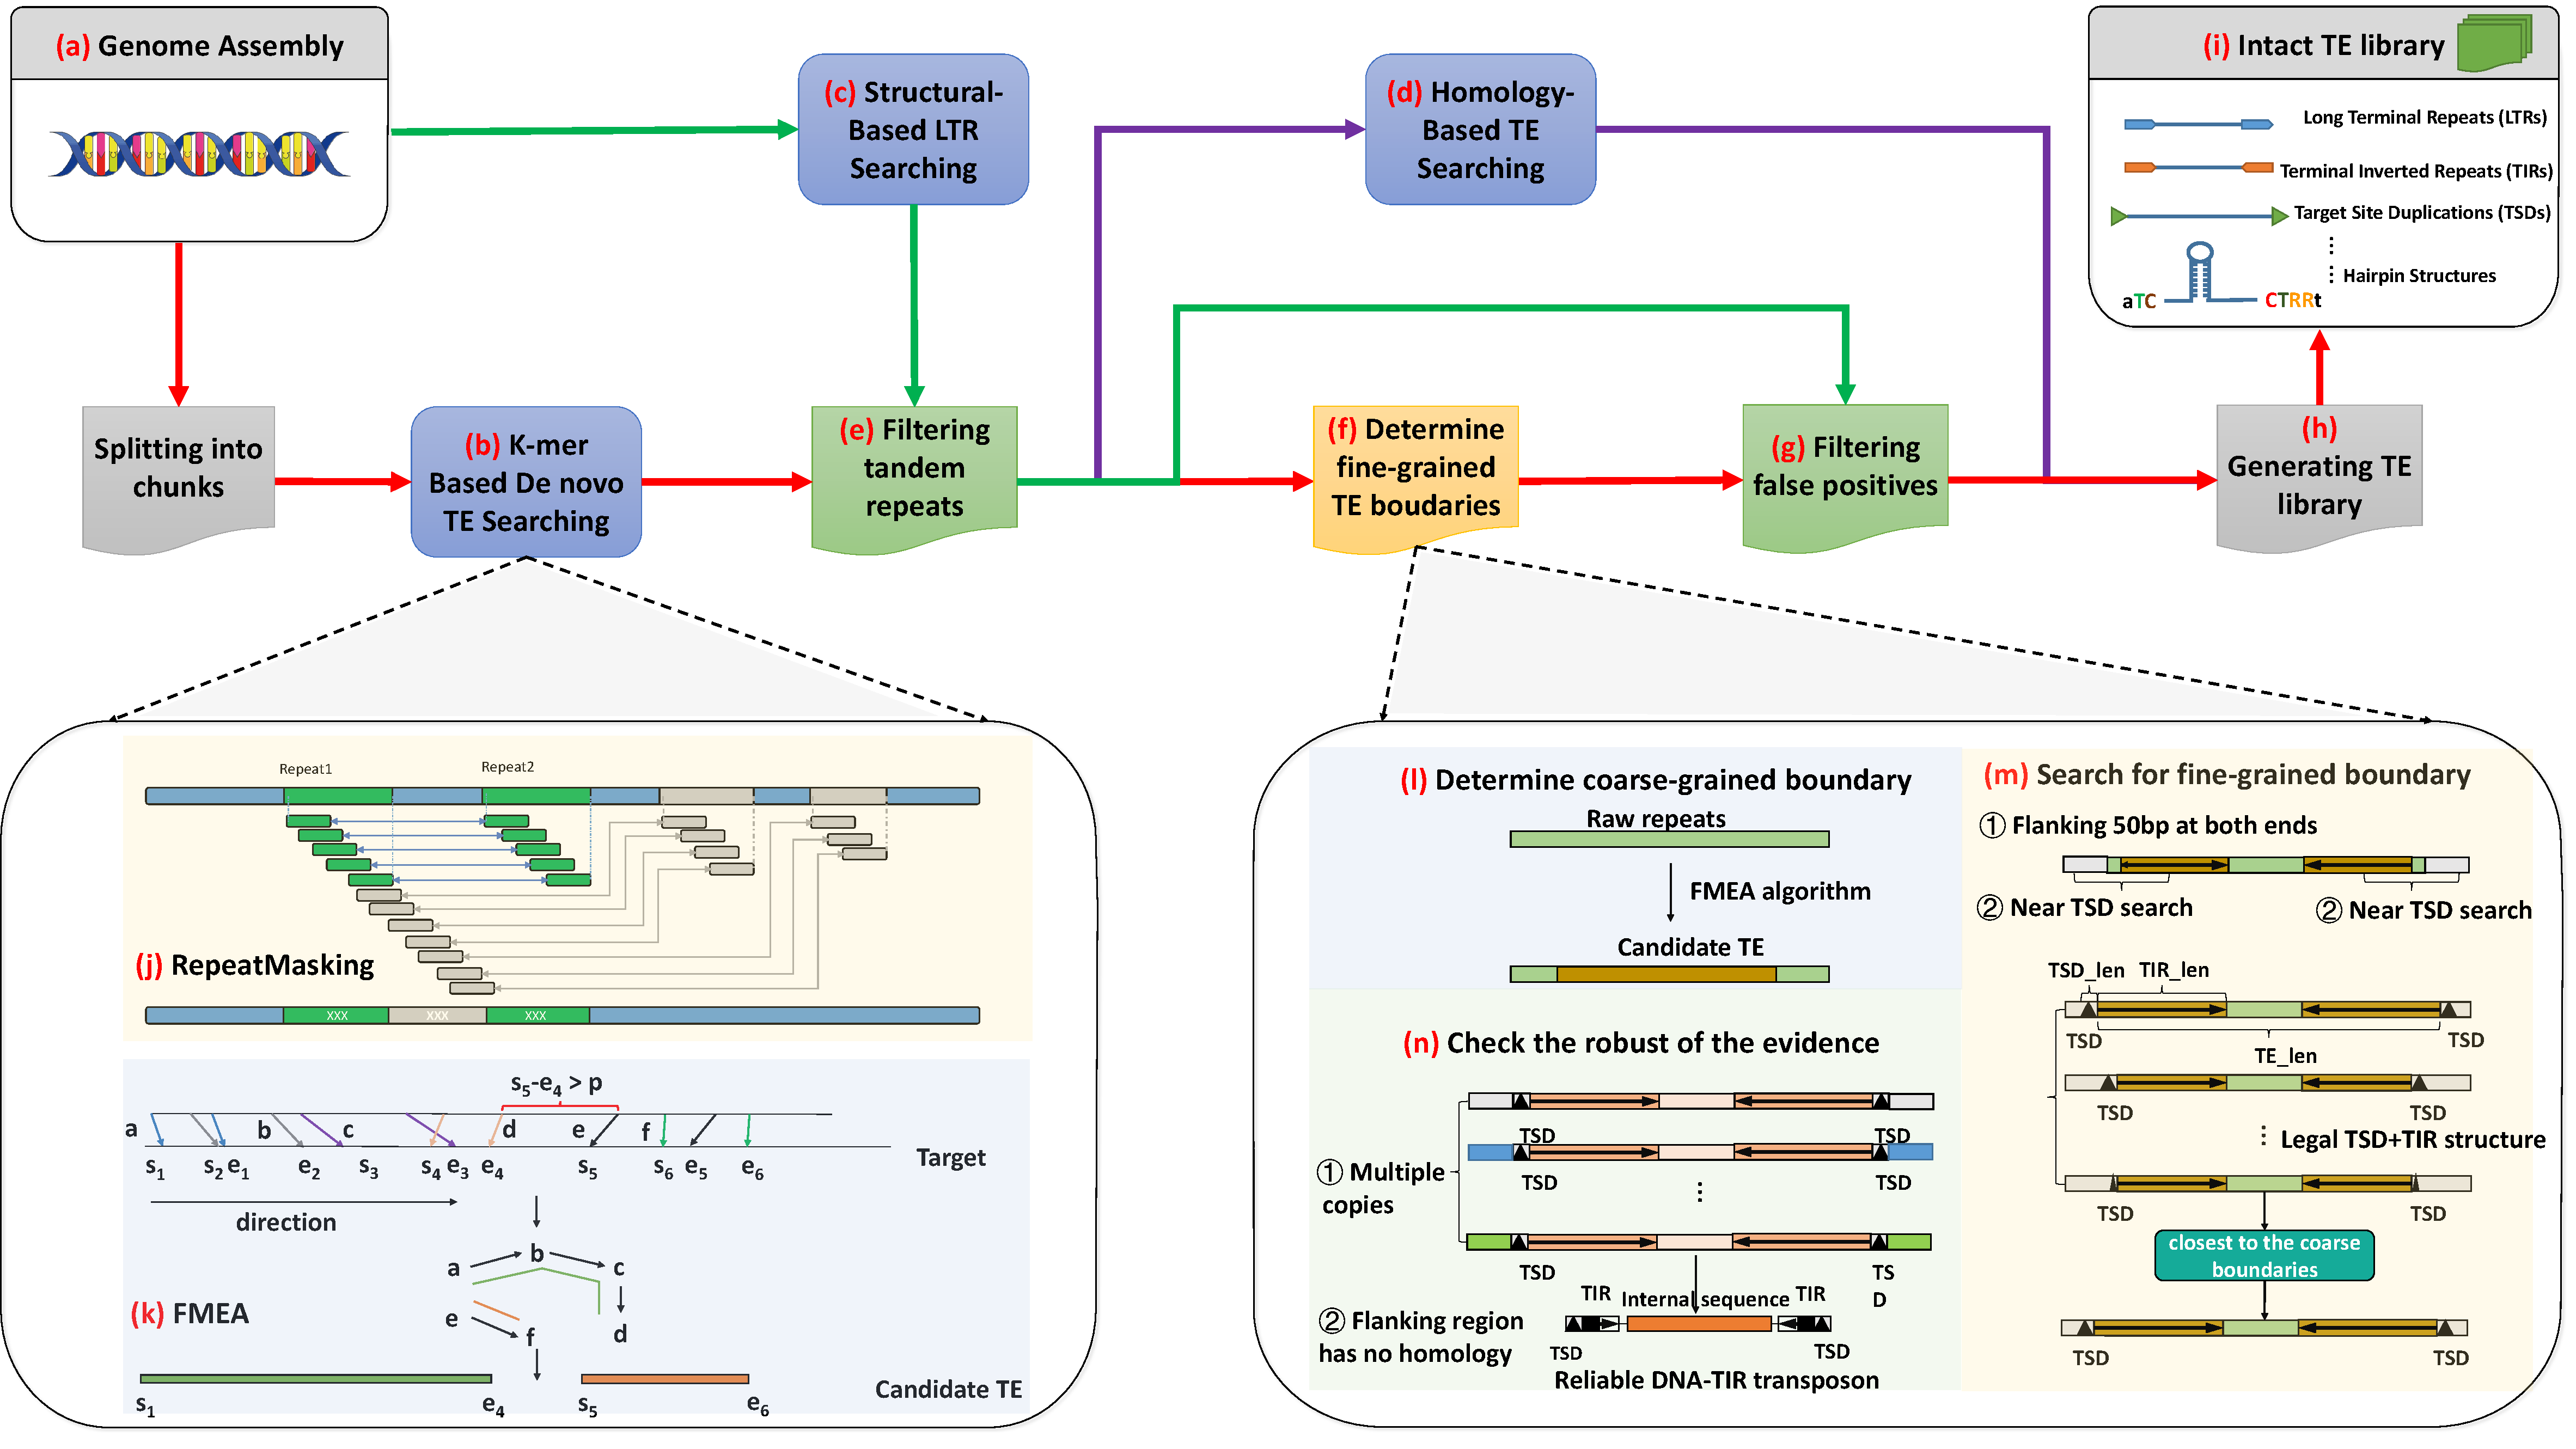
\includegraphics[width=1.0\textwidth]{figures/Framework1.pdf}}
	\caption{The workflow of HiTE. \textbf{a} HiTE takes the genome assembly as input; \textbf{b} the genome assembly is split into chunks to reduce the amount of single-round computation; \textbf{c, i, and j} three main modules of HiTE are used to identify different types of TEs; \textbf{d} the candidates with a large amount of tandem repeats are regarded as false positives and are filtered out; \textbf{e} the fine-grained boundaries of TEs are determined using signature-based methods; \textbf{f} the candidates with repetitive flanking sequences within copies that are parts of a larger repetitive element are considered false positives and are filtered out; \textbf{g} CD-HIT and RepeatClassifier are used to generate TE libraries; \textbf{h} the TE libraries generated by HiTE contain intact TE structures; \textbf{k} the candidate repeat regions within the genome are masked based on the low-frequency \emph{k}-mer masking method, RepeatMasking; \textbf{l} the coarse boundaries of TEs are identified based on the fault-tolerant mapping expansion algorithm, FMEA; and \textbf{m, n, and o} the true ends of TEs are discovered by searching for the fine-grained TE boundaries, and the robust evidence of true TEs are checked by non-homology flanking regions within multiple copies.}
	\label{fig:framework}
\end{figure}
\subsection*{HiTE Overview}
HiTE is an automated TE annotation pipeline that aims to produce a high-quality and structurally intact TE library. Purely \emph{de novo} methods, which detect TEs by sequence repetition alone, may miss low-copy but well-characterized TEs. At the same time, it is inevitable that they will include non-TE sequences, such as processed pseudogenes and high-copy gene families. Signature-based methods, in turn, identify TE instances by recognizing features of specific families of TEs, which always suffer from false positives due to the weak structural characteristics of some TEs. A TE discovery pipeline can overcome the shortcomings of any one particular approach by integrating a variety of existing tools into a single pipeline. However, using these existing tools directly will introduce their inherent errors (fragmentation or false positives) that will propagate to the whole genome annotation.
For the different structural characteristics and distribution of TEs in the genome, we employ three modules, \emph{k}-mer-based \emph{de novo} TE searching, structural-based LTR searching, and homology-based TE searching, to identify almost all types of transposons, including LTRs, TIRs, Helitrons, LINEs, and SINES.

Due to intraelement recombination and mutations, intact LTR-RTs contribute only a small fraction of all LTR-related sequences in a genome\cite{ou2018ltr_retriever, ou2018assessing}. In addition, long insertions are also more likely to be selectively disadvantageous to the genome, and full-length LTR elements are often reduced to solo LTRs via LTR–LTR recombination\cite{storer2022methodologies, jedlicka2020can}. To identify reliable LTR-RTs, we use the mature tools LTR\_FINDER\cite{xu2007ltr_finder} and LTRharvest\cite{ellinghaus2008ltrharvest} to find all candidate LTR candidates, followed by the LTR\_retriever\cite{ou2018ltr_retriever}, the state-of-the-art in LTR identification, as a stringent filtering method for the raw results by identifying LTR-specific signals.

TIR and Helitron elements have weak structure signals, which makes it easy to generate a large number of false positives. TIR elements, for example, may be structured with short terminal inverted repeats (5-27 bp for the hAT superfamily) and target site duplications (TSDs). Helitron elements have a short hairpin structure lying a few nucleotides before the 3$'$ end, with clearly defined 5$'$-TC and CTRR-3$'$ motifs (where R is a purine). To find the true ends of TIRs and Helitrons, we have developed a high-precision identification method, shown in Fig. \ref{fig:framework}.

Like the traditional \emph{de novo} method, HiTE can discover novel TE families. More importantly, it can accurately identify the structurally intact TE families by using highly conservative structural features and copy support. At the same time, the accurate definition of the boundaries reduces a large amount of manual repair.

\subsection*{Setting up benchmarking methods for TE library evaluation}
In eukaryotic genomes, transposable elements (TEs) exist widely in the form of both full-length (structurally intact) and fragmented sequences. An ideal library should contain only full-length models of all significantly distinct TEs that have left copies in the genome \cite{storer2022methodologies}, which are then used to detect fragmented and divergent TE sequences that are hard to recognize using structural features. However, compared with the limited number of full-length TE sequences, fragmented sequences are more abundant and comprise the majority of TEs, creating a challenge for algorithms to find their true ends.

The identification methods based on sequence repeatedness tend to produce more fragmented TE sequences, and their sequence boundaries are often approximate, which still need extensive editing before they can be accepted in curated databases such as Dfam or Repbase\cite{storer2022methodologies, bell2022transposable}. For example, the majority of TE models in Dfam come from libraries generated by RepeatModeler, and the great majority of Dfam submissions are currently housed in a non-curated section\cite{storer2021dfam}. Structure-based methods can clearly define the boundaries of the TE structure, but always with a high number of false positives.

To evaluate the performance of different TE identification methods, a high diversity of benchmarking approaches has been proposed, which is a barrier to the understanding of the true performance of methods\cite{storer2022methodologies}. For example, many benchmarking methods promote getting the higher metrics, including the higher copy number of TE, the higher number of models generated, the longer sequences of output, and even the higher N50, which does not take into account the quality of the TE library produced.

An ideal benchmarking method should consider both the integrity of TE structures and the false-positive rate of the TE library. To address this issue, we use the benchmarking methods released in two recent studies, EDTA\cite{ou2019benchmarking} and RepeatModeler2\cite{flynn2020repeatmodeler2} (BM\_EDTA and BM\_RM2 hereafter), which give ten metrics including \emph{Sensitivity}, \emph{Specificity}, \emph{Accuracy}, \emph{Precision}, \emph{FDR}, \emph{F1}, \emph{Perfect}, \emph{Good}, \emph{Present}, and \emph{Not\_found} (Additional File 1: Fig. S1).

%\subsection*{Setting up benchmarking methods for TE library evaluation}
%To fairly and comprehensively measure the quality of TE libraries generated by different TE identification tools, we use the benchmarking methods released in two recent studies, EDTA and RepeatModeler2. For convenience, we hereafter refer to the benchmarking methods of EDTA and RepeatModeler2 as BM\_EDTA and BM\_RM2, respectively. 
%
%As shown in Fig. S1(A), the BM\_EDTA evaluates the performance of various tools by annotating the genome with the gold standard TE library and the tested TE library generated by these tools. Based on the total number of genomic DNA bases, six metrics, including sensitivity, specificity, accuracy, precision, FDR, and F1, are used to characterize the annotation performance of the tested library\cite{ou2019benchmarking}. The BM\_EDTA can display detailed metrics, including the rates of false positives, which are common in many TE identification methods. However, it cannot reflect the integrity of the TE models. All general repeat identification programs, even those with many fragments and unclear boundaries, still performed well in benchmarking\cite{ou2019benchmarking}. For example, while a 1 kbp intact TE sequence and ten 100 bp fragments may obtain the same performance, the former is obviously more valuable in terms of TE integrity and biological significance.
%
%As shown in Fig. S1(B), the BM\_RM2 aligns the tested TE library with the gold standard library and divides the gold standard sequences into four levels: ``Perfect", ``Good", ``Present", and ``Not\_found". ``Perfect" families are those for which one sequence in the tested library matches with $>$95\% sequence similarity and $>$95\% length coverage to a family consensus in the gold standard library. ``Good" families are those in which multiple overlapping sequences in the tested library match with $>$95\% similarity and $>$95\% coverage to the curated consensus. A family is considered ``present" if one or multiple library sequences align with $>$80\% similarity and $>$80\% coverage to the reference consensus sequence. Below these thresholds, a family is considered ``not found"\cite{flynn2020repeatmodeler2}. The BM\_RM2 takes the integrity of the sequence into consideration. Intact TE models usually get a perfect level, while fragments can only get a good, present, or even not found level. However, it cannot display the rate of false positives in the tested TE library. By combining the two complementary benchmarking methods, we can accurately evaluate the integrity of TE models and the rate of false positives in the whole TE library.


\subsection*{Selecting benchmarking model species}
Despite the universality and importance of TEs in genomes, except for a few model species, the annotation and research of TEs in other species are still poor. In this benchmarking, we mainly focus on 4 typical species: Oryza sativa, Caenorhabditis briggsae, Drosophila melanogaster, and Danio rerio, whose TE libraries are well studied and preserved. These four species cover different sizes of genomes and divergent TE landscapes. The C. briggsae genome is the smallest and is dominated by DNA transposons; the D. melanogaster genome is dominated by LTR and LINE transposons; the Oryza sativa has a medium-sized genome with a similar proportion of LTR and DNA transposons; and the D. rerio has the largest genome, which comprises the majority of DNA transposons but also some LTR transposons.

Repbase Update (RU) is a database of representative repeat sequences in eukaryotic genomes that has a long history of TE discovery and annotation since 1992\cite{bao2015repbase}. RU has long been used as a manually curated reference database for nearly all eukaryotic genome sequence analyses. Here, we used TE libraries from RepBase26.05 as the gold standard for all species. The RepBase libraries were then used to annotate the genomes for both structurally intact and fragmented TE sequences, which comprised 47.81\% of the O. sativa genome, 15.83\% of the C. briggsae genome, 20.28\% of the D. melanogaster genome, and 57.36\% of the D. rerio genome, respectively (Table \ref{repbase_genome}). 

\begin{table}[h!]
	\caption{TE content in the benchmarking genomes.}\label{repbase_genome}
	\setlength{\tabcolsep}{2.5 mm}{
		\renewcommand{\arraystretch}{1.5}
	\begin{tabular}{cccccc}
		\hline
		& & Class & RepBase26.05  & Number of elements & Total (\%)\\ \hline
		\multirow{5}{*}{O. sativa*} &
		LTR & Class I & 88.4 Mb & 46595 & 23.61 \\
		& Non-LTR & Class I & 5.7 Mb & 13381 & 1.51 \\
		& TIR & Class II  & 67.7 Mb & 230281 & 18.09 \\
		& Helitron & Class II & 17.2 Mb & 66469 & 4.60 \\
		& Total & - & 179.0 Mb & 356726 & 47.81 \\ \hline  
		\multirow{5}{*}{C. briggsae*} &
		LTR & Class I & 0.2 Mb & 234 & 0.2 \\
		& Non-LTR & Class I & 0.9 Mb & 3085 & 0.59 \\
		& TIR & Class II  & 14.5 Mb & 68146 & 13.41 \\
		& Helitron & Class II & 1.8 Mb & 8509 & 1.63 \\
		& Total & - & 17.4 Mb & 79974 & 15.83 \\ \hline
		\multirow{5}{*}{D. melanogaster*} &
		LTR & Class I & 19.9 Mb & 21050 & 11.78 \\
		& Non-LTR & Class I & 10.8 Mb & 15428 & 6.37 \\
		& TIR & Class II  & 2.6 Mb & 6204 & 1.53 \\
		& Helitron & Class II & 1.0 Mb & 4822 & 0.60 \\
		& Total & - & 34.2 Mb & 47504 & 20.28 \\ \hline
		\multirow{5}{*}{D. rerio*} &
		LTR & Class I & 119.0 Mb & 296556 & 7.09 \\
		& Non-LTR & Class I & 74.3 Mb & 215393 & 4.42 \\
		& TIR & Class II  & 719.4 Mb & 3372500 & 42.84 \\
		& Helitron & Class II & 50.5 Mb & 178913 & 3.01 \\
		& Total & - & 963.2 Mb & 4063362 & 57.36 \\ \hline
	\end{tabular}
	\begin{tablenotes}
		\item[1] *Oryza sativa Japonica Group ``assembly IRGSP-1.0"
		\item[2] *Caenorhabditis briggsae ``assembly CB4"
		\item[3] *Drosophila melanogaster ``assembly Release 6 plus ISO1 MT"
		\item[4] *Danio rerio ``assembly GRCz11"
	\end{tablenotes}
	}
\end{table}

\begin{figure}[h!]
	\centerline{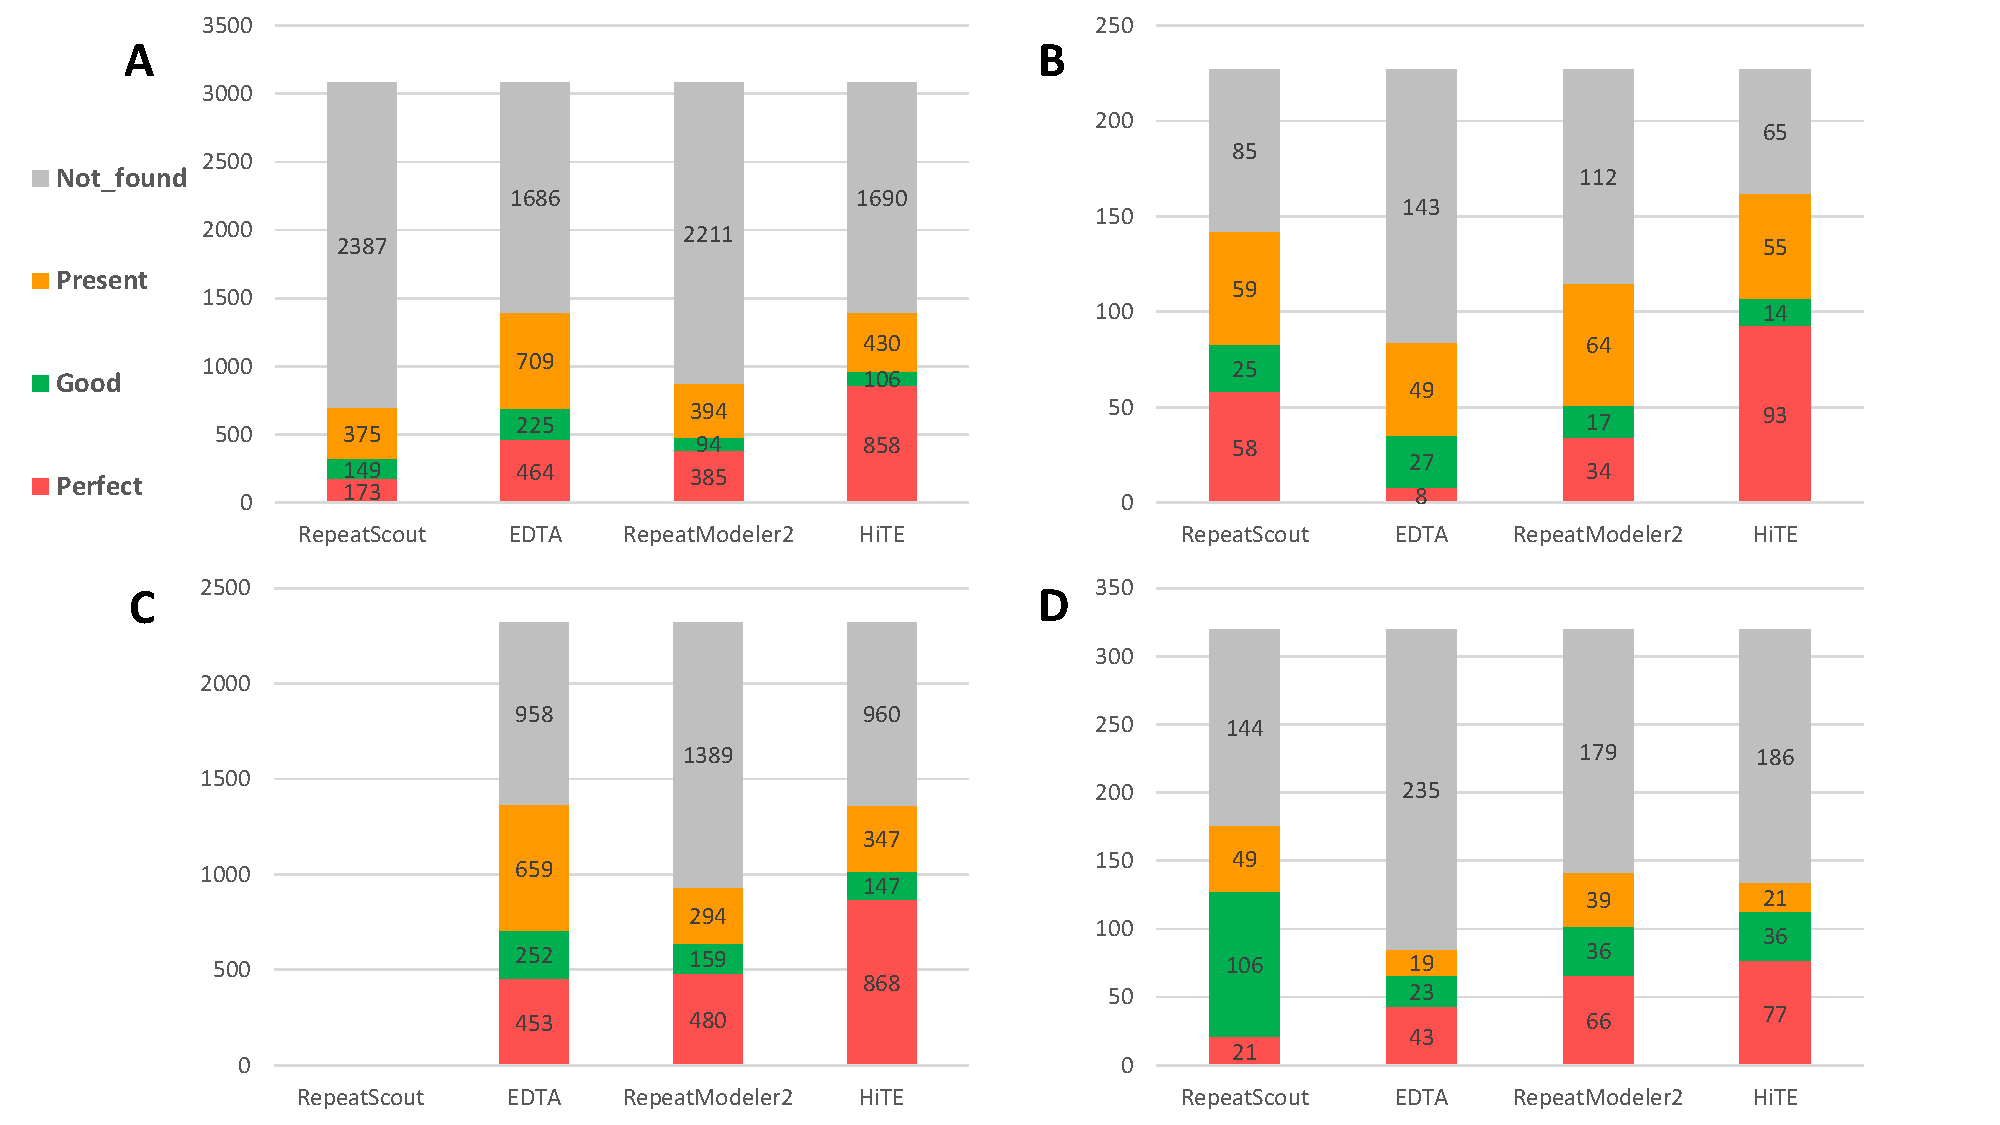
\includegraphics[width=1.0\textwidth]{figures/RM2Results.pdf}}
	\caption{Performance of general-purpose TE annotators based on benckmarking method of RepeatModeler2. \textbf{a} Performance based on O. sativa genome. \textbf{b} Performance based on C. briggsae genome. \textbf{c} Performance based on D. rerio genome. \textbf{d} Performance based on D. melanogaster genome.}
	\label{fig:rm2_results}
\end{figure}

\begin{figure}[h!]
	\centerline{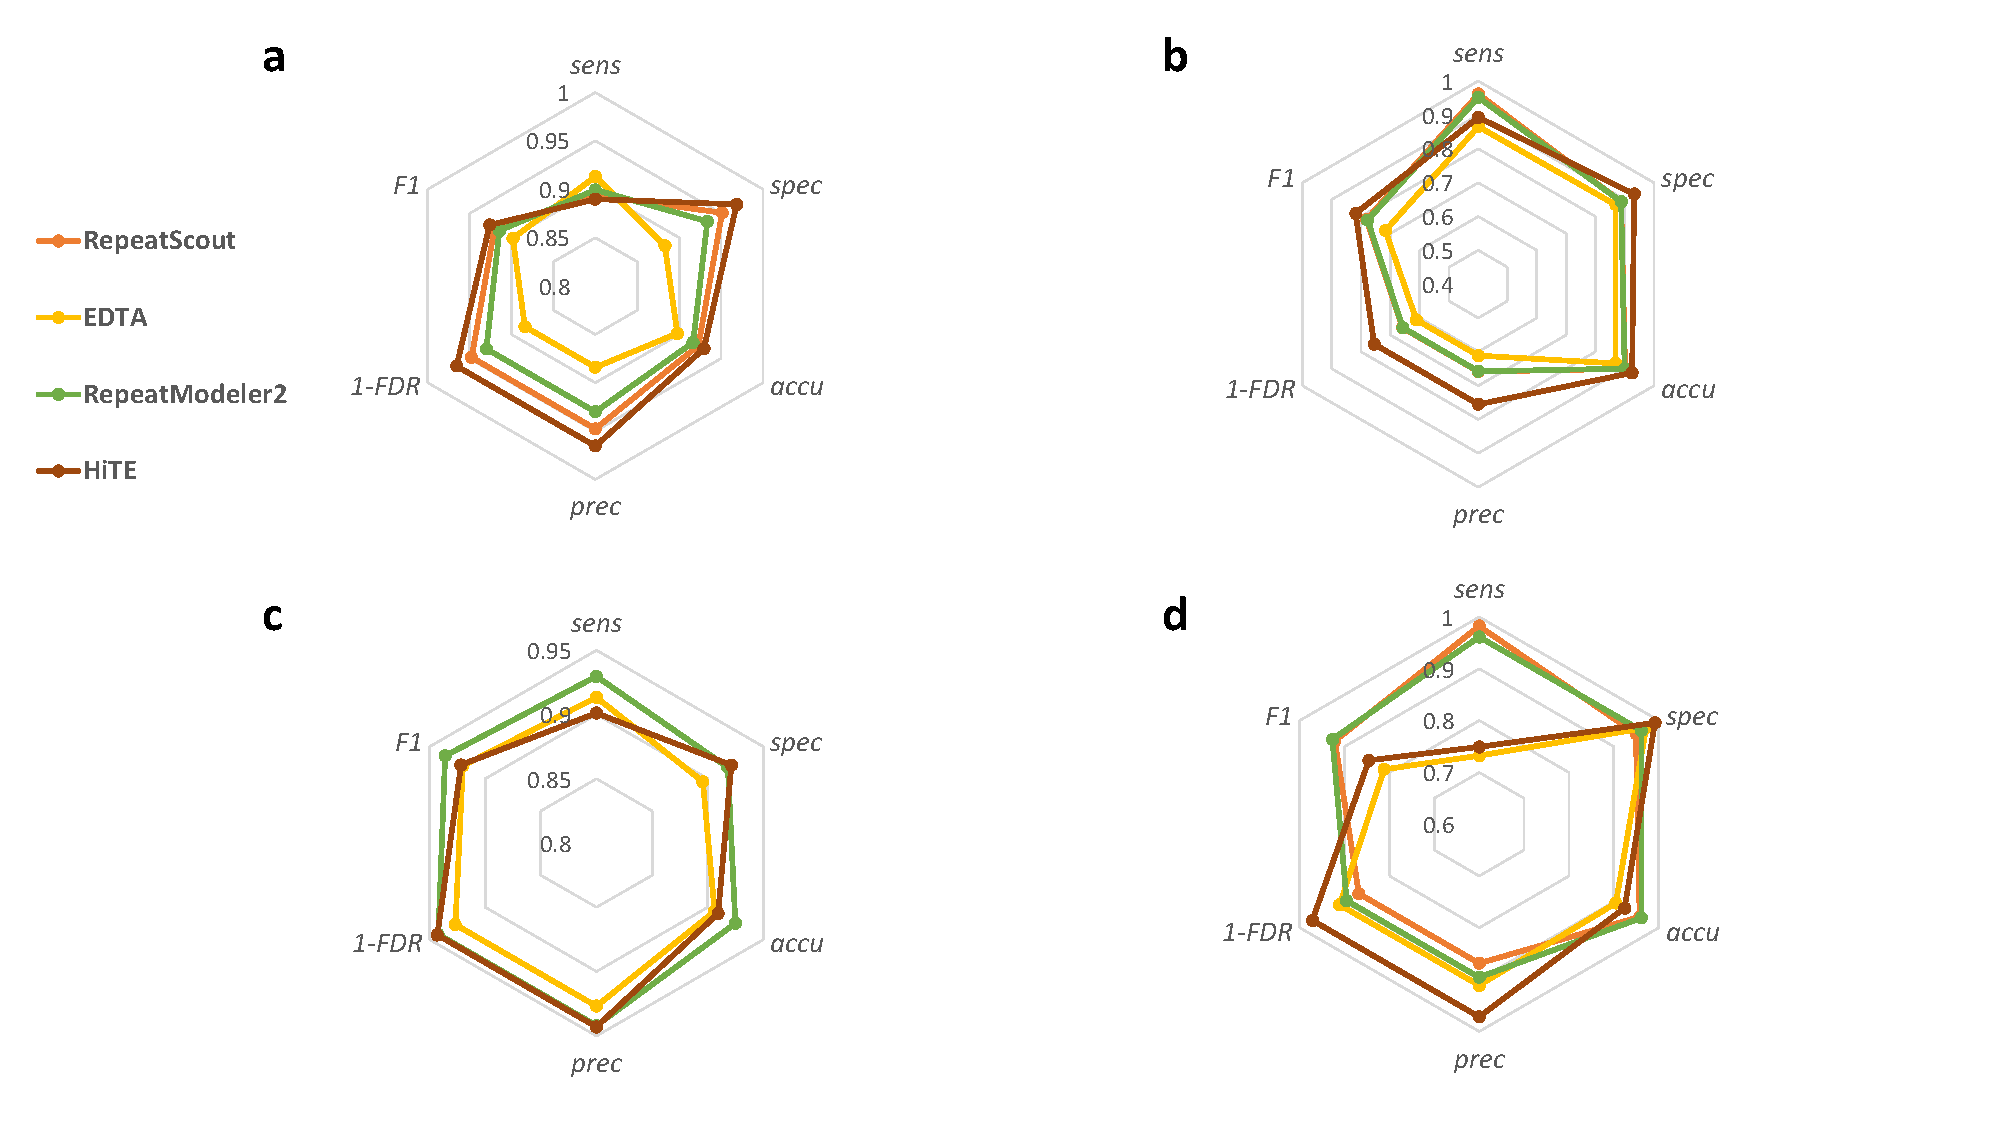
\includegraphics[width=1.0\textwidth]{figures/EDTAResults.pdf}}
	\caption{Performance of general-purpose TE annotators based on benckmarking method of EDTA.  \textbf{a} Performance based on O. sativa genome. \textbf{b} Performance based on C. briggsae genome. \textbf{c} Performance based on D. rerio genome. \textbf{d} Performance based on D. melanogaster genome.}
	\label{fig:edta_results}
\end{figure}

\subsection*{HiTE benchmarking for different species}
We compared HiTE with the other three mainstream general-purpose TE annotators, including RepeatScout, EDTA, and RepeatModeler2. To date, EDTA is the best annotation tool based on structure signals, and RepeatModeler2 is the pipeline with the best overall performance. RepeatScout was originally used to identify repetitive sequences, and its algorithm characteristics tend to find highly consistent repetitive regions, such as duplicates or the youngest TE families. %For older and more divergent TEs, many fragments are often generated. 
RepeatModeler, the old version of RepeatModeler2, uses RECON and RepeatScout for \emph{de novo} TE identification. Although RECON uses the single linkage clustering algorithm to generate TE sequences based on overlapping alignments, accurate clustering of these alignments is challenging due to the high fragmentation and mosaicism present in TE families\cite{storer2022methodologies}. Due to the limited ability to generate structurally intact TE models, RepeatModeler2 adds the LTR\_retriever module to generate structurally intact LTR transposons, which greatly increases its performance\cite{flynn2020repeatmodeler2}.

The benchmarking results using BM\_RM2 are shown in Fig. \ref{fig:rm2_results} (Additional file 2: Table S1). Among these methods, we found that RepeatModeler2 achieved good performance and was stable on all datasets. The performance of EDTA is unstable instead, producing a high number of \emph{Perfect} models on the TE-rich genomes, such as O. sativa, but a low number on the other genomes. At the same time, the number of \emph{Presents} models generated by EDTA is significantly higher than that of other tools, indicating many fragments may exist. RepeatScout produced more \emph{Perfect} models on C. briggsae, which suggest that the majority of TE in the C. briggsae genome are relatively young. However, when it comes to other species, RepeatScout obtained the minimum number of \emph{Perfect} models. Since RepeatScout cannot process more than 1 GB of genomes, it has no results for D. rerio. Notably, HiTE produced the highest number of \emph{Perfect} TE models than other tools on all datasets and a smaller number of \emph{Good} and \emph{Present} TE models, which shows that HiTE can restore more gold standard TE models and fewer fragments. %we found that all tools have quite a few ``Not\_Found" TE models, and we discussed in \textbf{Section Discussion}.

As shown in Fig. \ref{fig:edta_results} (Additional file 2: Table S1), we noticed that RepeatScout and RepeatModeler2 both achieved a consistently high performance using BM\_EDTA, which is also described in the EDTA\cite{ou2019benchmarking}. The greatest advantage of the BM\_EDTA is that it can intuitively describe the false positive rate of the tested TE library, but it cannot reflect the integrity of the TE models. For example, in O. sativa and D. melanogaster, RepeatScout obtained the lowest number of \emph{Perfect} TE models, indicating that there are a large number of fragments, but it still achieved a high BM\_EDTA performance. Instead, HiTE showed somewhat lower sensitivity but significantly higher precision performance, including \emph{Precision}, \emph{Specificity}, and \emph{Accuracy}, which indicates that HiTE can identify more accurate TE.  At the same time, since the BM\_EDTA is based on base statistics, some false-positive sequences with short length can be well aligned to the true TEs, resulting in falsely high sensitivity but significantly low precision. Like the structure-based method EDTA, HiTE produces a similar lower sensitivity, which does not neccessary mean that HiTE or EDTA discover fewer TE models than RepeatScout and RepeatModeler2. On the contrary, HiTE produces more \emph{Perfect} and fewer \emph{Not\_found} TE models using the BM\_RM2, which indicates more gold standard TE models are restored.

\begin{figure}[h!]
	\centerline{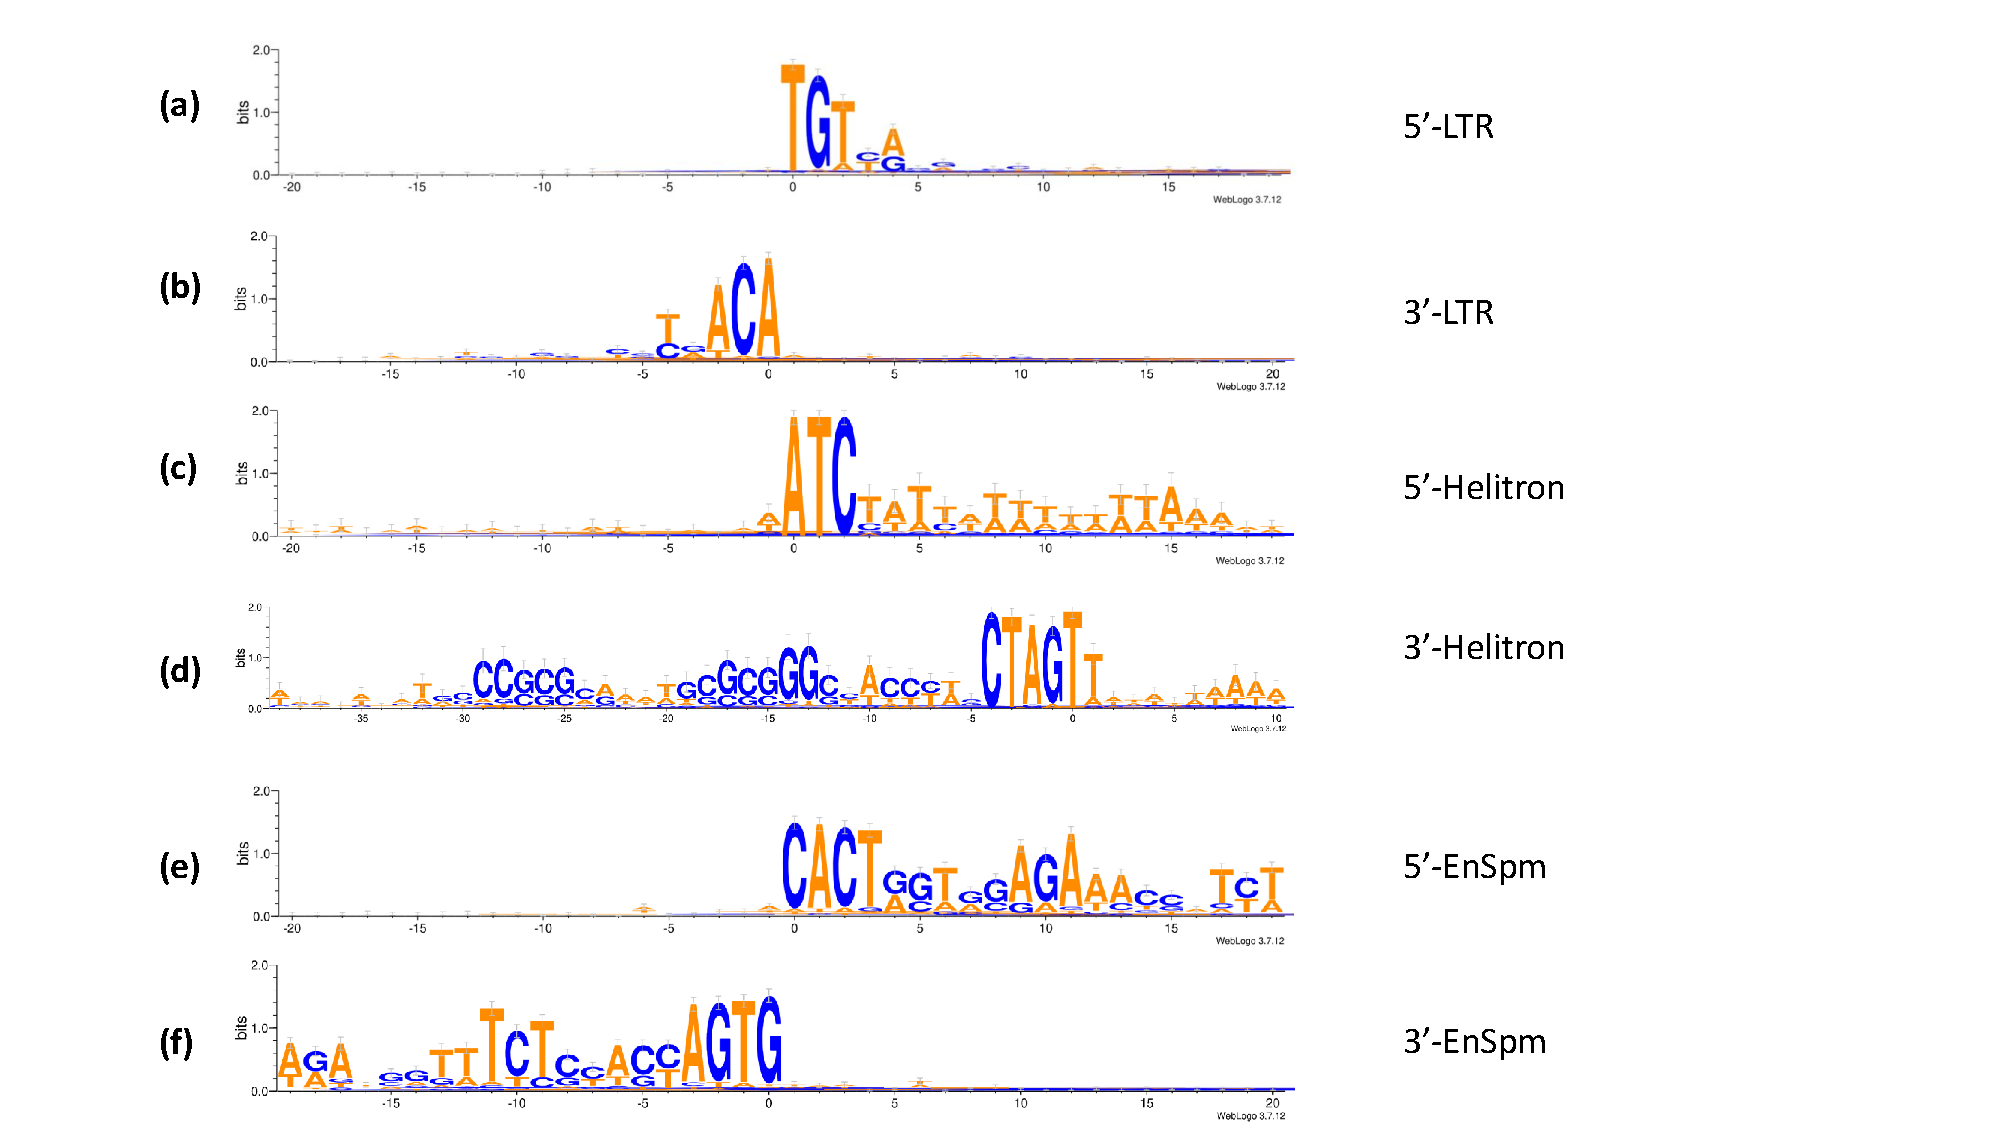
\includegraphics[width=1.0\textwidth]{figures/SeqLogos.pdf}}
	\caption{Sequence logos of terminal and flanking sequences of LTR, Helitron, and EnSpm candidates generated by HiTE. \textbf{(a)} 5$'$ terminal of LTR candidates with the starting position labeled as 0; \textbf{(b)} 3$'$ terminal of LTR candidates with the last position labeled as 0; \textbf{(c)} 5$'$ terminal of Helitron candidates with the starting position labeled as 1; \textbf{(d)} 3$'$ terminal of Helitron candidates with the last position labeled as -1; \textbf{(e)} 5$'$ terminal of EnSpm candidates with the starting position labeled as 0; \textbf{(f)} 3$'$ terminal of EnSpm candidates with the last position labeled as 0. Sequence logos are produced by WebLogo\cite{crooks2004weblogo}.}
	\label{fig:seq_logos}
\end{figure}

\begin{figure}[h!]
	\centerline{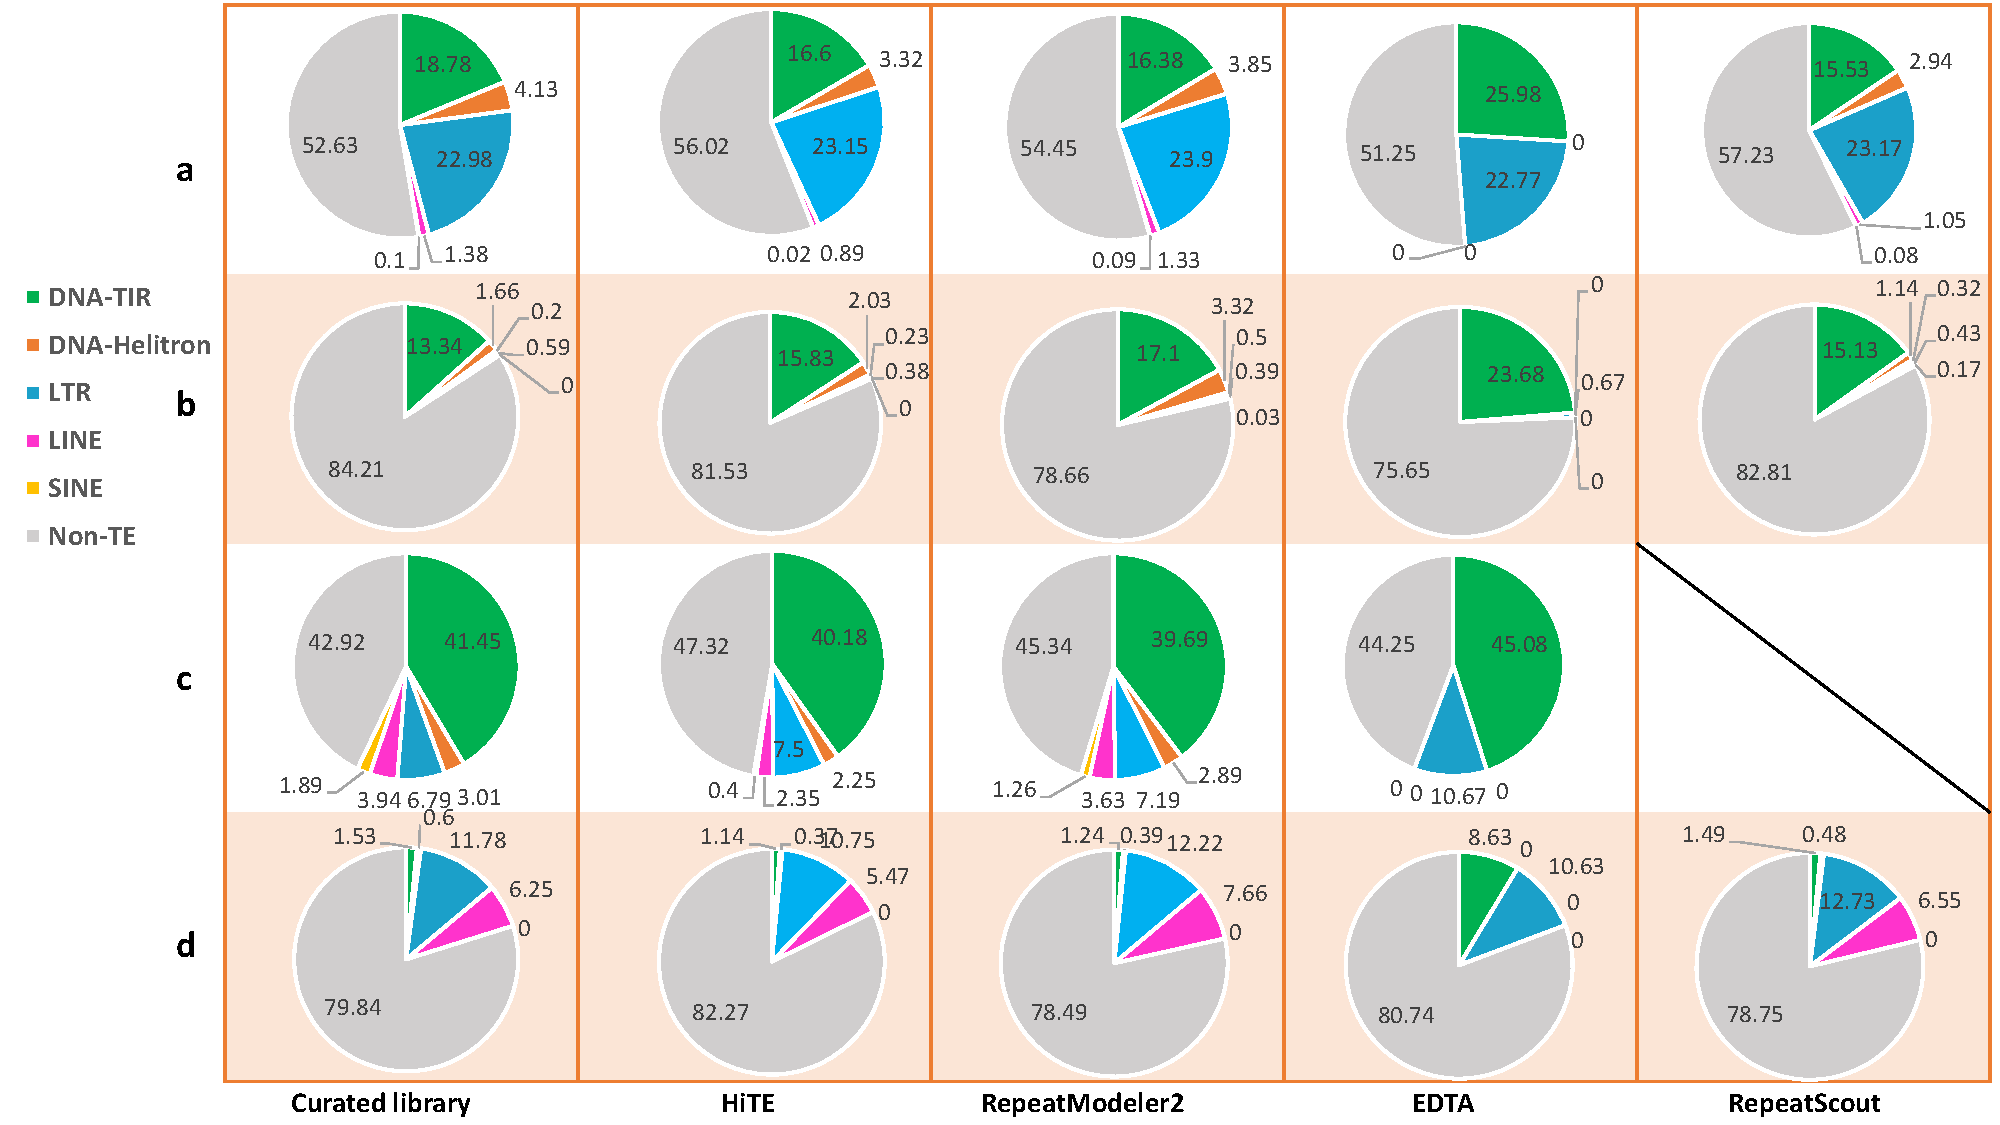
\includegraphics[width=1.0\textwidth]{figures/RatioResults.pdf}}
	\caption{Percent of genome masked by each major subclass based on five types of TE libraries, generated by manually curated, HiTE, RepeatModeler2, EDTA, and RepeatScout, respectively. \textbf{a} The percentage of the O. sativa genome masked by TE libraries. \textbf{b} The percentage of the C. briggsae genome masked by TE libraries. \textbf{c} The percentage of the D. rerio genome masked by TE libraries. \textbf{d} The percentage of the D. melanogaster genome masked by TE libraries. }
	\label{fig:ratio_results}
\end{figure}

\subsection*{TEs discovered by HiTE are consistent with previous studies}
To identify sequence motifs of typical TEs, we aligned both terminals and flanking sequences of LTR, Helitron, and EnSpm identified by HiTE and produced sequence logos that represent the nucleotide usage at each position in both terminals and their flanking regions (Fig. \ref{fig:seq_logos}). As previously documented\cite{zhou2021comprehensive}, LTRs are typically flanked by 2-bp palindromic motifs, commonly 5$'$-TG...CA-3$'$, which is shown in Fig. \ref{fig:seq_logos}a, b. Helitrons are always inserted into 5$'$-AT-3$'$ target sites and do not have terminal inverted repeats. As shown in Fig. \ref{fig:seq_logos}c, d, we clearly discovered the canonical terminal structure 5$'$-TC...CTRR-3$'$ (with 5$'$-TC...CTAG-3$'$ dominating) in Helitrons that are inserted into 5$'$-AT-3$'$ target sites. We also noticed a significantly higher AT content in the 5$'$ terminal and enriched CG content at the 3$'$ terminal, especially at the $-$29 and $-$13 positions, which could produce a canonical Helitron feature, a hairpin loop, consistent with previous observations\cite{yang2009structure, xiong2014helitronscanner}. Furthermore, as shown in Fig. \ref{fig:seq_logos}e, f, we discovered highly conserved CACT(A/G) motifs in the short terminals of EnSpm elements that had previously been documented \cite{wicker2007unified, demarco2006smtrc1}. 

As an additional assessment of the ability for HiTE to discover known TEs in each of these genomes, we run RepeatMasker with each output library generated by different tools and measure the percentage of the genome masked by each major TE subclass. HiTE restores the TE landscapes of these species consistent with the reference libraries (Fig. \ref{fig:ratio_results}). The genome of O. sativa is known to contain DNA-TIR and LTR elements in close proportions\cite{ou2019benchmarking}, which is recovered by our HiTE library (Fig. \ref{fig:ratio_results}a). As shown in Fig. \ref{fig:ratio_results}b, the HiTE library discovered a similar proportion to the reference library, which indicates an abundant percentage of DNA-TIR elements in the genome of C. briggsae\cite{harris1988sequence}. The genome of D. rerio is dominated by class II DNA-TIR transposons, but it also has a diverse composition of LTR retroelements with many distinct families (Fig. \ref{fig:ratio_results}c)\cite{howe2013zebrafish}. In addition, our results show that the genome of D. melanogaster is dominated by retrotransposons, especially LTR and LINE retroelements (Fig. \ref{fig:ratio_results}d)\cite{lerat2003sequence}. 


%Each TE sequence in HiTE has complete structural characteristics and copy verification (at least two full-length copies exist, and the region outside the TE copy boundary has no homology), which leads to high precision and somewhat lower sensitivity.
%The reason that RepeatScout and RepeatModeler2 can obtain higher sensitivity is that they identify TE based on the repeatedness of the sequence, so many short and incomplete TE models will also be identified, which are filtered out in HiTE.

%\begin{table}[h!]
%	\caption{Details of performance among general-purpose repeat annotators based on O. sativa.}\label{total_result_rice}
%	\setlength{\tabcolsep}{0.15 mm}{
%		\renewcommand{\arraystretch}{1.5}
%		\begin{tabular}{cccccccccccc}
%			\hline
%			\multirow{2}{*}{Tools} & \multicolumn{6}{c}{EDTA evaluation} & & \multicolumn{4}{c}{RepeatModeler2 evaluation} \\
%			\cline{2-7} \cline{9-12} 
%			& Sensitivity & Specificity & Accuracy & Precision & FDR & F1 &  & Perfect & Good & Present & Not\_found \\
%			\hline
%			HiTE & 0.8897 & 0.9686 & 0.9295 & 0.9653 & 0.0347 & 0.9260 & & 858 & 106 & 430 & 1690 \\
%			RepeatScout & 0.8940 & 0.9514 & 0.9230 & 0.9476 & 0.0524 & 0.9200 & & 173 & 149 & 375 & 2387  \\
%			EDTA & 0.9131 & 0.8831 & 0.8979 & 0.8840 & 0.1160 & 0.8983 & & 464 & 225 & 709 & 1686 \\
%			RepeatModeler2 & 0.8993 & 0.9336 & 0.9166 & 0.9299 & 0.0701 & 0.9144 & & 385 & 94 & 394 & 2211 \\ 
%			\hline
%	\end{tabular} }
%\end{table}
%
%\begin{table}[h!]
%	\caption{Details of performance among general-purpose repeat annotators based on C. briggsae.}\label{total_result_cb}
%	\setlength{\tabcolsep}{0.15 mm}{
%		\renewcommand{\arraystretch}{1.5}
%		\begin{tabular}{cccccccccccc}
%			\hline
%			\multirow{2}{*}{Tools} & \multicolumn{6}{c}{EDTA evaluation} & & \multicolumn{4}{c}{RepeatModeler2 evaluation} \\
%			\cline{2-7} \cline{9-12} 
%			& Sensitivity & Specificity & Accuracy & Precision & FDR & F1 &  & Perfect & Good & Present & Not\_found \\
%			\hline
%			HiTE & 0.8926 & 0.9323 & 0.9247 & 0.7550 & 0.2450 & 0.8181 & & 93 & 14 & 55 & 65 \\
%			RepeatScout & 0.9616 & 0.8875 & 0.9011 & 0.6583 & 0.3417 & 0.7815 & & 58 & 25 & 59 & 85 \\
%			EDTA & 0.8656 & 0.8690 & 0.8683 & 0.6115 & 0.3885 & 0.7167 & & 8 & 27 & 49 & 143 \\
%			RepeatModeler2 & 0.9519 & 0.8876 & 0.8995 & 0.6576 & 0.3424 & 0.7778 & & 34 & 17 & 64 & 112 \\ 
%			\hline
%	\end{tabular} }
%\end{table}
%
%\begin{table}[h!]
%	\caption{Details of performance among general-purpose repeat annotators based on D. rerio.}\label{total_result_zebrafish}
%	\setlength{\tabcolsep}{0.15 mm}{
%		\renewcommand{\arraystretch}{1.5}
%		\begin{tabular}{cccccccccccc}
%			\hline
%			\multirow{2}{*}{Tools} & \multicolumn{6}{c}{EDTA evaluation} & & \multicolumn{4}{c}{RepeatModeler2 evaluation} \\
%			\cline{2-7} \cline{9-12} 
%			& Sensitivity & Specificity & Accuracy & Precision & FDR & F1 &  & Perfect & Good & Present & Not\_found \\
%			\hline
%			HiTE & 0.9012 & 0.9213 & 0.9094 & 0.9430 & 0.0570 & 0.9216 & & 868 & 147 & 347 & 960 \\
%			RepeatScout & - & - & - & - & - & - & & - & - & - & -  \\
%			EDTA & 0.9134 & 0.8955 & 0.9061 & 0.9268 & 0.0732 & 0.9201 & & 453 & 252 & 659 & 958  \\
%			RepeatModeler2 & 0.9297 & 0.9180 & 0.9249 & 0.9421 & 0.0579 & 0.9359 & & 480 & 159 & 294 & 1389 \\ 
%			\hline
%	\end{tabular} }
%\end{table}
%
%\begin{table}[h!]
%	\caption{Details of performance among general-purpose repeat annotators based on D. melanogaster.}\label{total_result_dmel}
%	\setlength{\tabcolsep}{0.15 mm}{
%		\renewcommand{\arraystretch}{1.5}
%		\begin{tabular}{cccccccccccc}
%			\hline
%			\multirow{2}{*}{Tools} & \multicolumn{6}{c}{EDTA evaluation} & & \multicolumn{4}{c}{RepeatModeler2 evaluation} \\
%			\cline{2-7} \cline{9-12} 
%			& Sensitivity & Specificity & Accuracy & Precision & FDR & F1 &  & Perfect & Good & Present & Not\_found \\
%			\hline
%			HiTE & 0.7491 & 0.9917 & 0.9243 & 0.9718 & 0.0282 & 0.8461 & & 77 & 36 & 21 & 186 \\
%			RepeatScout & 0.9824 & 0.9493 & 0.9577 & 0.8685 & 0.1315 & 0.9220 & & 21 & 106 & 49 & 144 \\
%			EDTA & 0.7322 & 0.9721 & 0.9046 & 0.9113 & 0.0887 & 0.8120 & & 43 & 23 & 19 & 235 \\
%			RepeatModeler2 & 0.9614 & 0.9613 & 0.9613 & 0.8956 & 0.1044 & 0.9273 & & 66 & 36 & 39 & 179 \\  
%			\hline
%	\end{tabular} }
%\end{table}

\begin{figure}[h!]
	\centerline{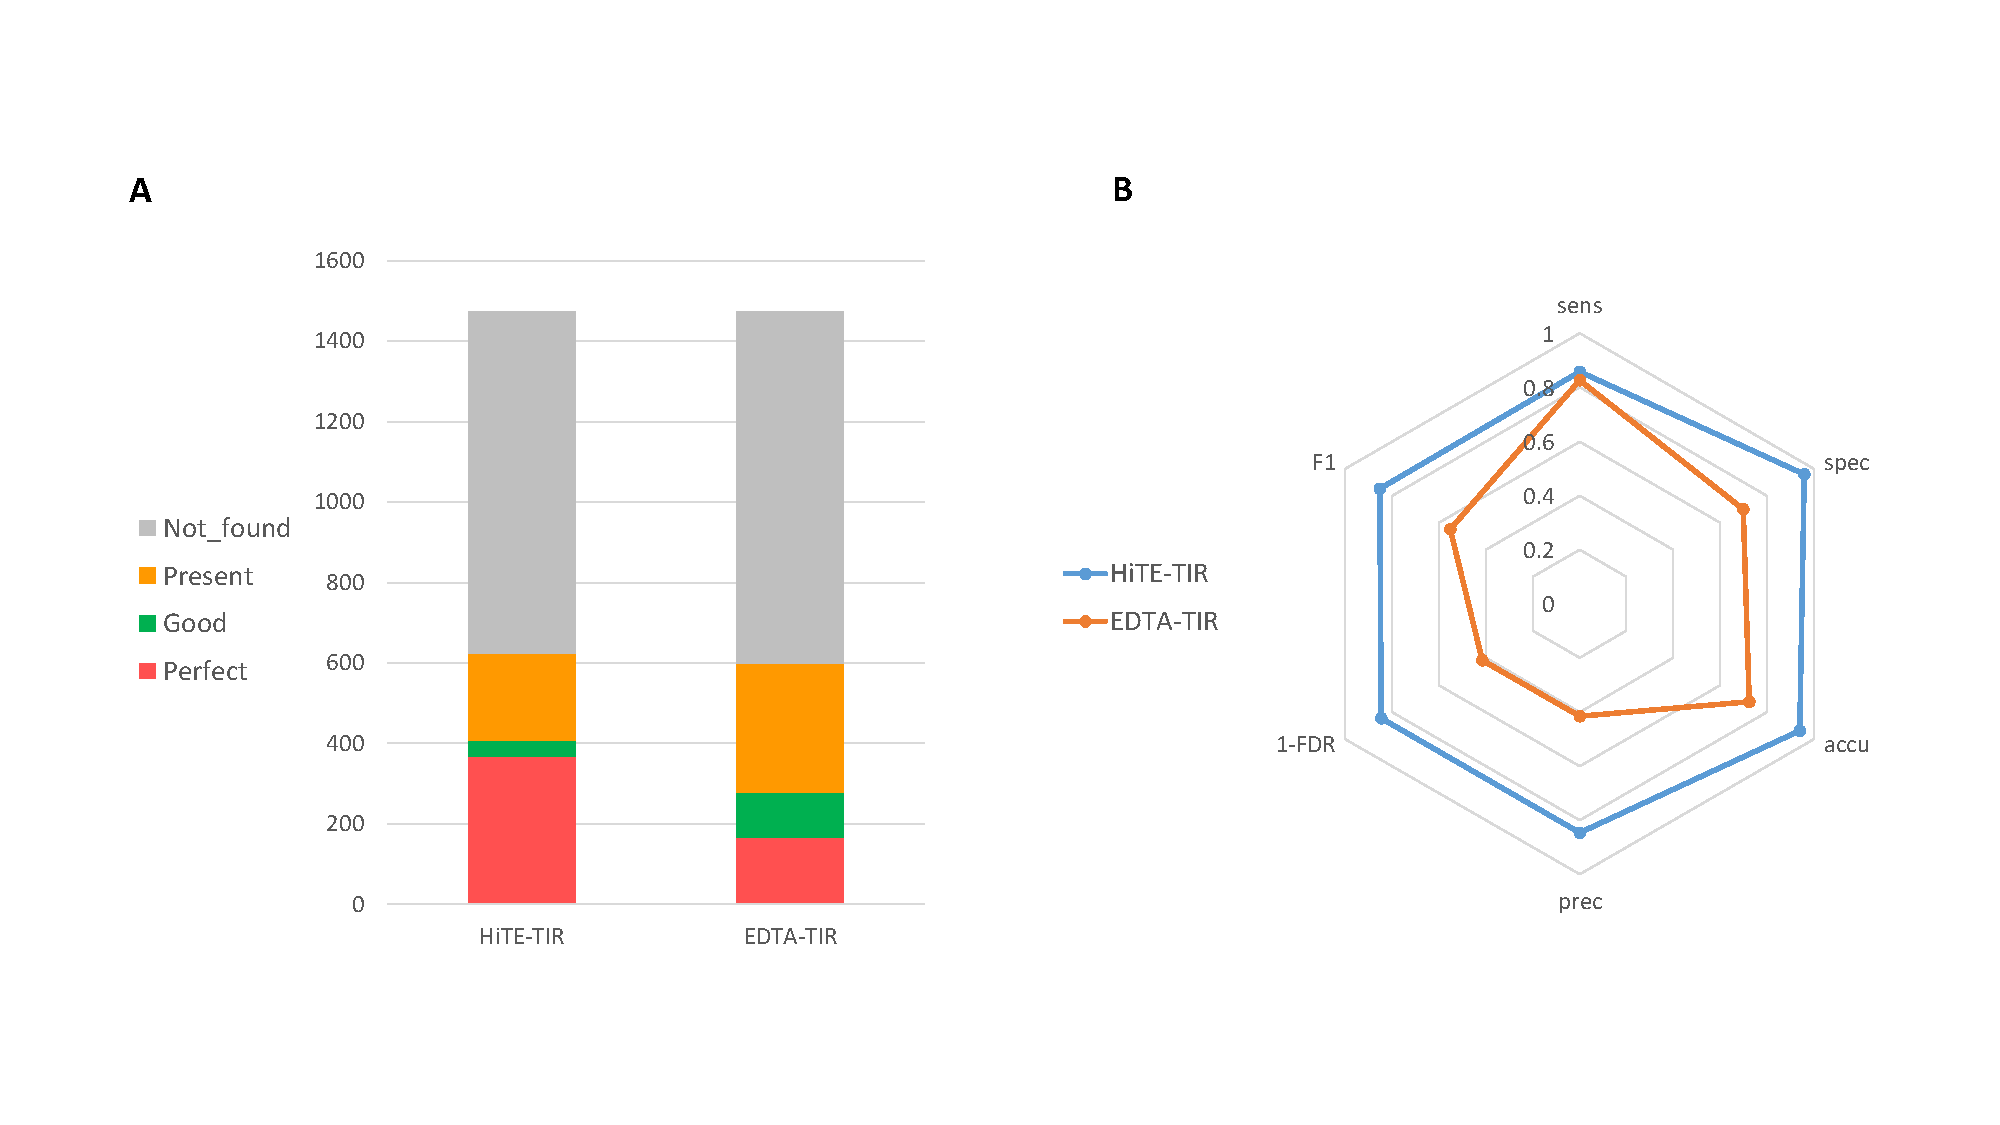
\includegraphics[width=1.0\textwidth]{figures/TIRResults.pdf}}
	\caption{Performance of TIR annotators. \textbf{a} the performance based on benckmarking method of RepeatModeler2 and \textbf{b} the performance based on benckmarking method of EDTA.}
	\label{fig:tir_results}
\end{figure}

\subsection*{Performance comparison for TIR element detection}
TIR elements, which belong to class II TEs, are ancient TEs found in almost all eukaryotes. They are flanked by characteristic terminal inverted repeat sequences (TIRs), usually presenting in low to moderate numbers\cite{wicker2007unified}. TIR elements may contribute to genome evolution by generating allelic diversity, inducing structural variation, and regulating gene expression\cite{su2019tir}. TIR elements are divided into nine known superfamilies by the distinguished TIRs and the size of TSDs (usually 2–11 bp). However, the  identification and annotation of TIR elements are quite challenging due to the short TIRs. For example, members of the hAT superfamily have TSDs of 8 bp and relatively short TIRs of 5–27 bp\cite{kempken2001hat}.

Many tools have been designed for the identification of TIR elements using structural signals, such as IRF\cite{warburton2004inverted}, TIRvish\cite{gremme2013genometools}, TIR-Learner\cite{su2019tir}, and GRF\cite{shi2019generic}, which are comprehensively evaluated in EDTA, and most of them are proven to discover a high number of false positives\cite{ou2019benchmarking}. For example, the IRF and GRF-TIR produce a large number of candidates, with 4.7 GB and 630 GB (13x–1684x the size of the 374 MB rice genome, respectively) of raw TIR candidates. Although the TIR module (GRF and TIR-learner) of EDTA has demonstrated great promise for structural annotation and achieved higher performance than other tools\cite{ou2019benchmarking}, it is far from satisfactory. To solve this problem, we developed a new method to achieve high-precision identification of TIR elements (see the \textbf{``Methods"} section).

As shown in Fig. \ref{fig:tir_results}a (Additional file 2: Table S2), according to the benchmarking results of the BM\_RM2, our method can identify more TE models labelled as \emph{Perfect} with a lower number of \emph{Good} and \emph{Present}. According to the benchmarking results of the BM\_EDTA, our method produces a higher sensitivity, specificity, accuracy, precision, F1, and a lower FDR than EDTA (Fig. \ref{fig:tir_results}b; Additional file 2: Table S2). These two benchmarking methods both demonstrate that our method can achieve high-precision identification of TIR elements.

%\begin{table}[h!]
%	\caption{Details of performance among all types of TE annotators based on O. sativa.}\label{all_TE_result_rice}
%	\setlength{\tabcolsep}{0.1 mm}{
%		\renewcommand{\arraystretch}{1.5}
%		\begin{tabular}{cccccccccccccc}
%			\hline
%			\multirow{2}{*}{TE class} & \multirow{2}{*}{Tools} & \multicolumn{6}{c}{EDTA evaluation} & & \multicolumn{4}{c}{RepeatModeler2 evaluation} \\
%			\cline{4-9} \cline{11-14} 
%			& & & Sens & Spec & Accu & Prec & FDR & F1 &  & Perfect & Good & Present & Not\_found \\
%			\hline
%			\multirow{2}{*}{TIR} & EDTA-TIR & & 0.8274 & 0.6989 & 0.7253 & 0.4149 & 0.5851 & 0.5526 & & 165 & 112 & 320 & 877  \\
%			& HiTE-TIR & & 0.8607 & 0.9591 & 0.9391 & 0.8431 & 0.1569 & 0.8518 & &  374 & 39 & 217 & 844 \\
%			\cline{2-14}
%			\multirow{3}{*}{Helitron} & EAHelitron & & 0.2666 & 0.9983 & 0.9135 & 0.9536 & 0.0464 & 0.4167 & & 0 & 0 & 0 & 310   \\
%			& \makecell{EDTA-\\HelitronScanner} & & 0.8930 & 0.6259 & 0.6509 & 0.1982 & 0.8018 & 0.3244 & & 4 & 30 & 54 & 222 \\
%			& HiTE-Helitron & & 0.7040 & 0.9703 & 0.9438 & 0.7240 & 0.2761 & 0.7138 & & 35 & 14 & 21 & 240  \\
%			\cline{2-14}
%			\multirow{3}{*}{LTR} & LTRharvest & & 0.9420 & 0.8269 & 0.8548 & 0.6356 & 0.3644 & 0.7590 & & 395 & 56 & 105 & 549  \\
%			& LTR\_FINDER & & 0.9676 & 0.8601 & 0.8860 & 0.6874 & 0.3126 & 0.8038 & & 493 & 68 & 117 & 427 \\
%			& LTR\_retriever & & 0.9604 & 0.9456 & 0.9491 & 0.8491 & 0.1509 & 0.9013 & & 417 & 46 & 172 & 470  \\
%			\cline{2-14}
%			\multirow{2}{*}{Non-LTR} & Non\_LTR\_library & & 0.7302 & 0.9879 & 0.9819 & 0.5883 & 0.4117 & 0.6516 & & 77 & 3 & 21 & 48  \\
%			& HiTE-Non-LTR & & 0.6519 & 0.9999 & 0.9916 & 0.9906 & 0.0094 & 0.7863 & &  24 & 0 & 21 & 104 \\
%			\hline
%	\end{tabular} }
%\end{table}



We have observed that some new TIR elements have been found, which differ significantly from those in Repbase and are distinguished by the 80\% principle\cite{wicker2007unified}. Through careful inspection, we found that these new TIR elements have complete TIRs and TSDs, and the boundaries between their copies are clear. Notably, most of them have low copy numbers (Fig. \ref{fig:novel_tirs}c). At the same time, nearly half of the TIR elements have more than 3 copies (Fig. \ref{fig:novel_tirs}b), suggesting that these are like real TEs that were not included in the Repbase library due to their low number of copies.
In addition, we recognize that some TIR elements have TIRs similar to the known TIRs in Repbase (Fig. \ref{fig:novel_tirs}a), which are likely to be non-autonomous TIR elements.

\begin{figure}[h!]
	\centerline{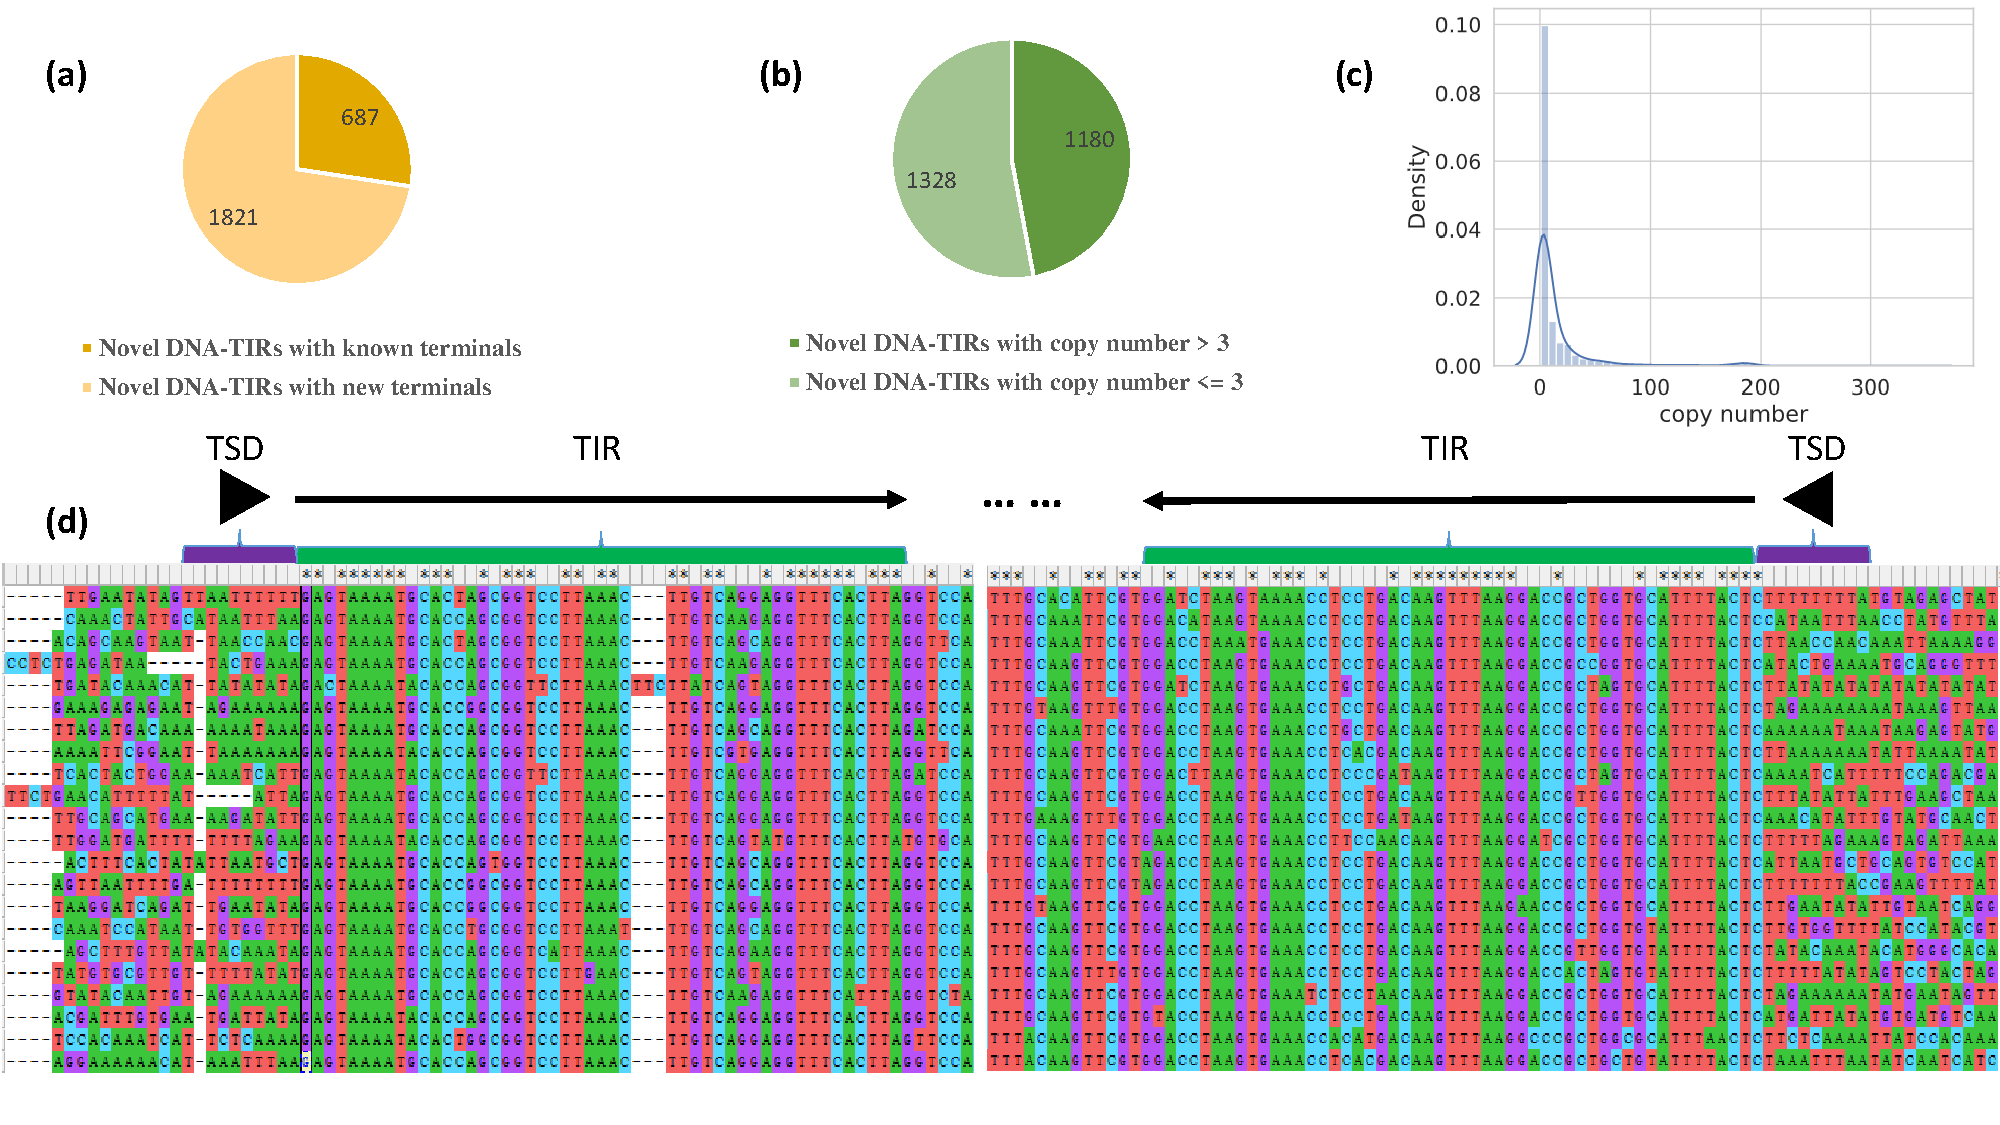
\includegraphics[width=1.0\textwidth]{figures/NovelTIRs.pdf}}
	\caption{Characteristic of novel TIR elements identified by HiTE. \textbf{a} the number of novel TIR elements with different types of terminals; \textbf{b} the number of novel TIR elements with copy numbers $>$ 3 and $<=$ 3; \textbf{c} the distribution of copy numbers of TIR elements identified by HiTE; and \textbf{d} the multiple sequence alignment example of a novel TIR element discovered by HiTE.}
	\label{fig:novel_tirs}
\end{figure}

\begin{figure}[h!]
	\centerline{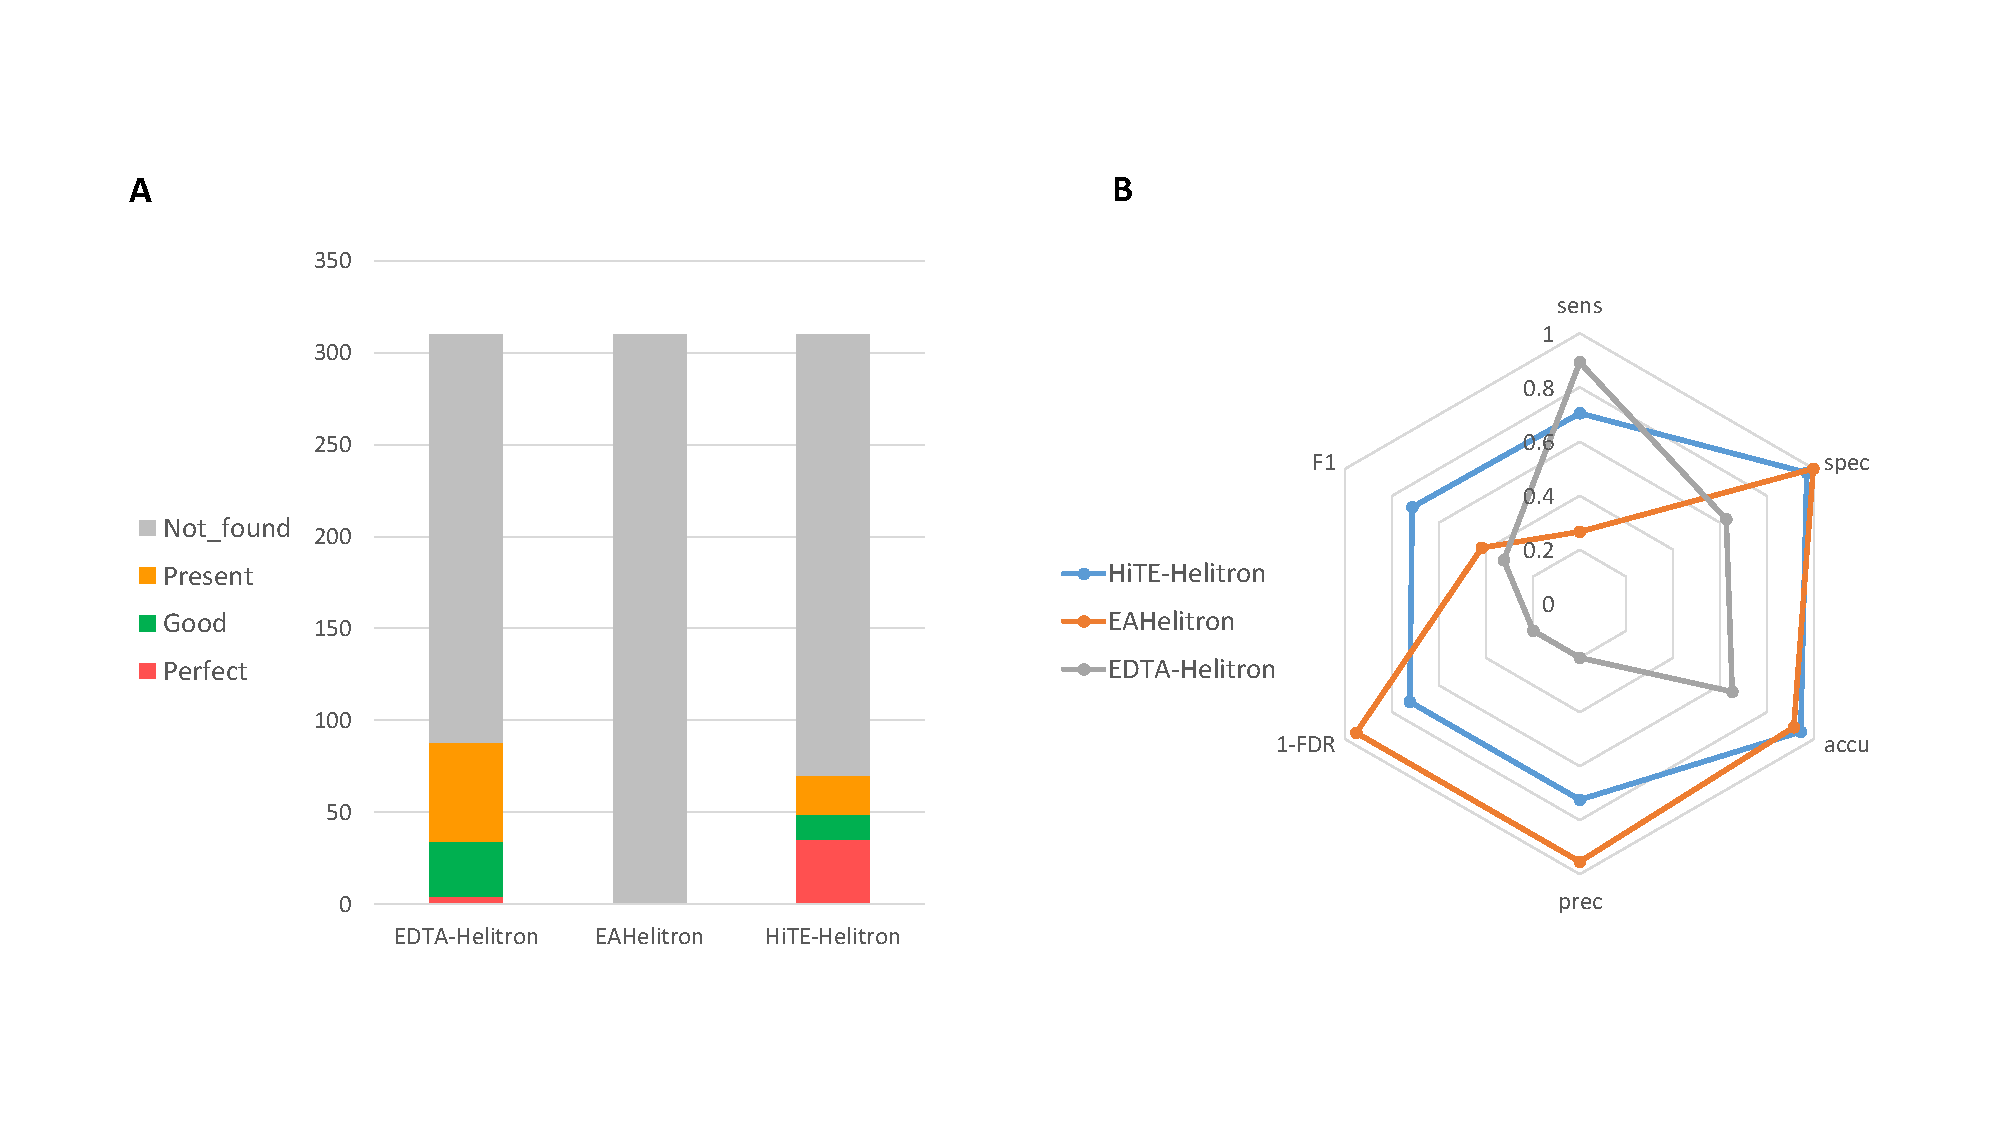
\includegraphics[width=1.0\textwidth]{figures/HelitronResults.pdf}}
	\caption{Performance of Helitron annotators. \textbf{a} the performance based on benckmarking method of RepeatModeler2 and \textbf{b} the performance based on benckmarking method of EDTA.}
	\label{fig:helitron_results}
\end{figure}

\subsection*{Performance comparison for Helitron element detection}
Helitron elements (Helitrons hereafter) are a subclass of DNA transposons, which replicate through the rolling circle mechanism. When replicating themselves, only the single strand of DNA is broken, and no TSD is generated, which is different from the other TEs. Helitrons have a 5$'$-TC...-CTRR-3$'$ conserved structure, where R refers to purine, A or G, and there is a short hairpin structure about 10 bp upstream of the 3' end. Helitrons mostly transition into host AT target sites, resulting in flanking 5$'$-A and 3$'$-T nucleus\cite{kapitonov2007helitrons}. However, the weak structural signals of Helitrons make identification of these elements particularly challenging.

To date, only two tools, HelitronScanner and EAHelitron, can produce useful Helitron predictions. HelitronScanner identifies the sequence patterns in Helitrons using the local combinational variable (LCV) algorithm, which produced a large number of candidate sequences, most of which are false positives. For example, 52 MB of raw candidate sequences cover 13.9\% of the rice genome, which obviously exceeds the real coverage ($\sim$4\%). EDTA filters the results of HelitronScanner, greatly improving its specificity and accuracy without reducing the sensitivity\cite{ou2019benchmarking}. Nevertheless, the precision of the Helitron identification module in EDTA is still very low (Fig. \ref{fig:helitron_results}b; Additional file 2: Table S2).

We also test the other tool, EAHelitron, which identifies Helitrons based on the conservative structure traits using regular expression (RE), such as the 5$'$ terminal with TC, the 3$'$ terminal with CTAGt, and a GC-rich hairpin loop before 2–10 nt of CTAG. The performance of EAHelitron is primarily determined by the pre-defined patterns of hairpin loop regular expressions. We observed that it lost some of the hairpin loop patterns of real Helitrons. For example, many real Helitrons in C. briggsae cannot be discovered until we manually add a new pattern of haripin loop ``[GC]{4}". EAHelitron specifies a ``-u" parameter to search all possible 5$'$-TC upstream of CTAGt-3$'$ (Additional file 2: Table S4), while it is hard to know the real 5$'$ end of Helitron. As suggested by the authors, we take the first 5$'$-TC closest to CTAGt-3$'$ as the 5$'$ end of candidate Helitrons, which leads to extremely short sequences with only 87 bp average length and 44 candidates in rice. The short candidate sequences produce the highest precision but the lowest sensitivity (Fig. \ref{fig:helitron_results}b; Additional file 2: Table S2). Moreover, it cannot restore any gold standard models according to the BM\_RM2 (Fig. \ref{fig:helitron_results}a; Additional file 2: Table S2).

To discover the intact Helitrons, we have developed a new Helitron identification method, which is a further usage of the coarse boundaries of TE candidates output by the FMEA algorithm (see the \textbf{``Methods"} section). EAHelitron is used to locate the accurate 3$'$-CTRR and the hairpin loop structure in candidate TE sequences. The 5$'$-TC closest to the coarse boundary is selected as the true end. To control the false discovery of the candidate Helitrons, we filtered out the candidates that were not inserted into AT target sites. Finally, the false positives are filtered out by homology outside the boundaries of copies.

The experimental results show that our Helitron identification method has the highest performance (Fig. \ref{fig:helitron_results}; Additional file 2: Table S2), which is superior to EDTA with significantly higher precision, specificity, and accuracy. Compared with the pure EAHelitron method, we have greatly improved the sensitivity and F1 value. At the same time, we identify more \emph{Perfect} Helitrons in the gold standard dataset. However, we do notice that our results are still affected by false positives, which indicates that our method has potential for improvement, and our sensitivity will be further improved once EAHelitron includes a more comprehensive hairpin loop pattern.

\begin{figure}[h!]
	\centerline{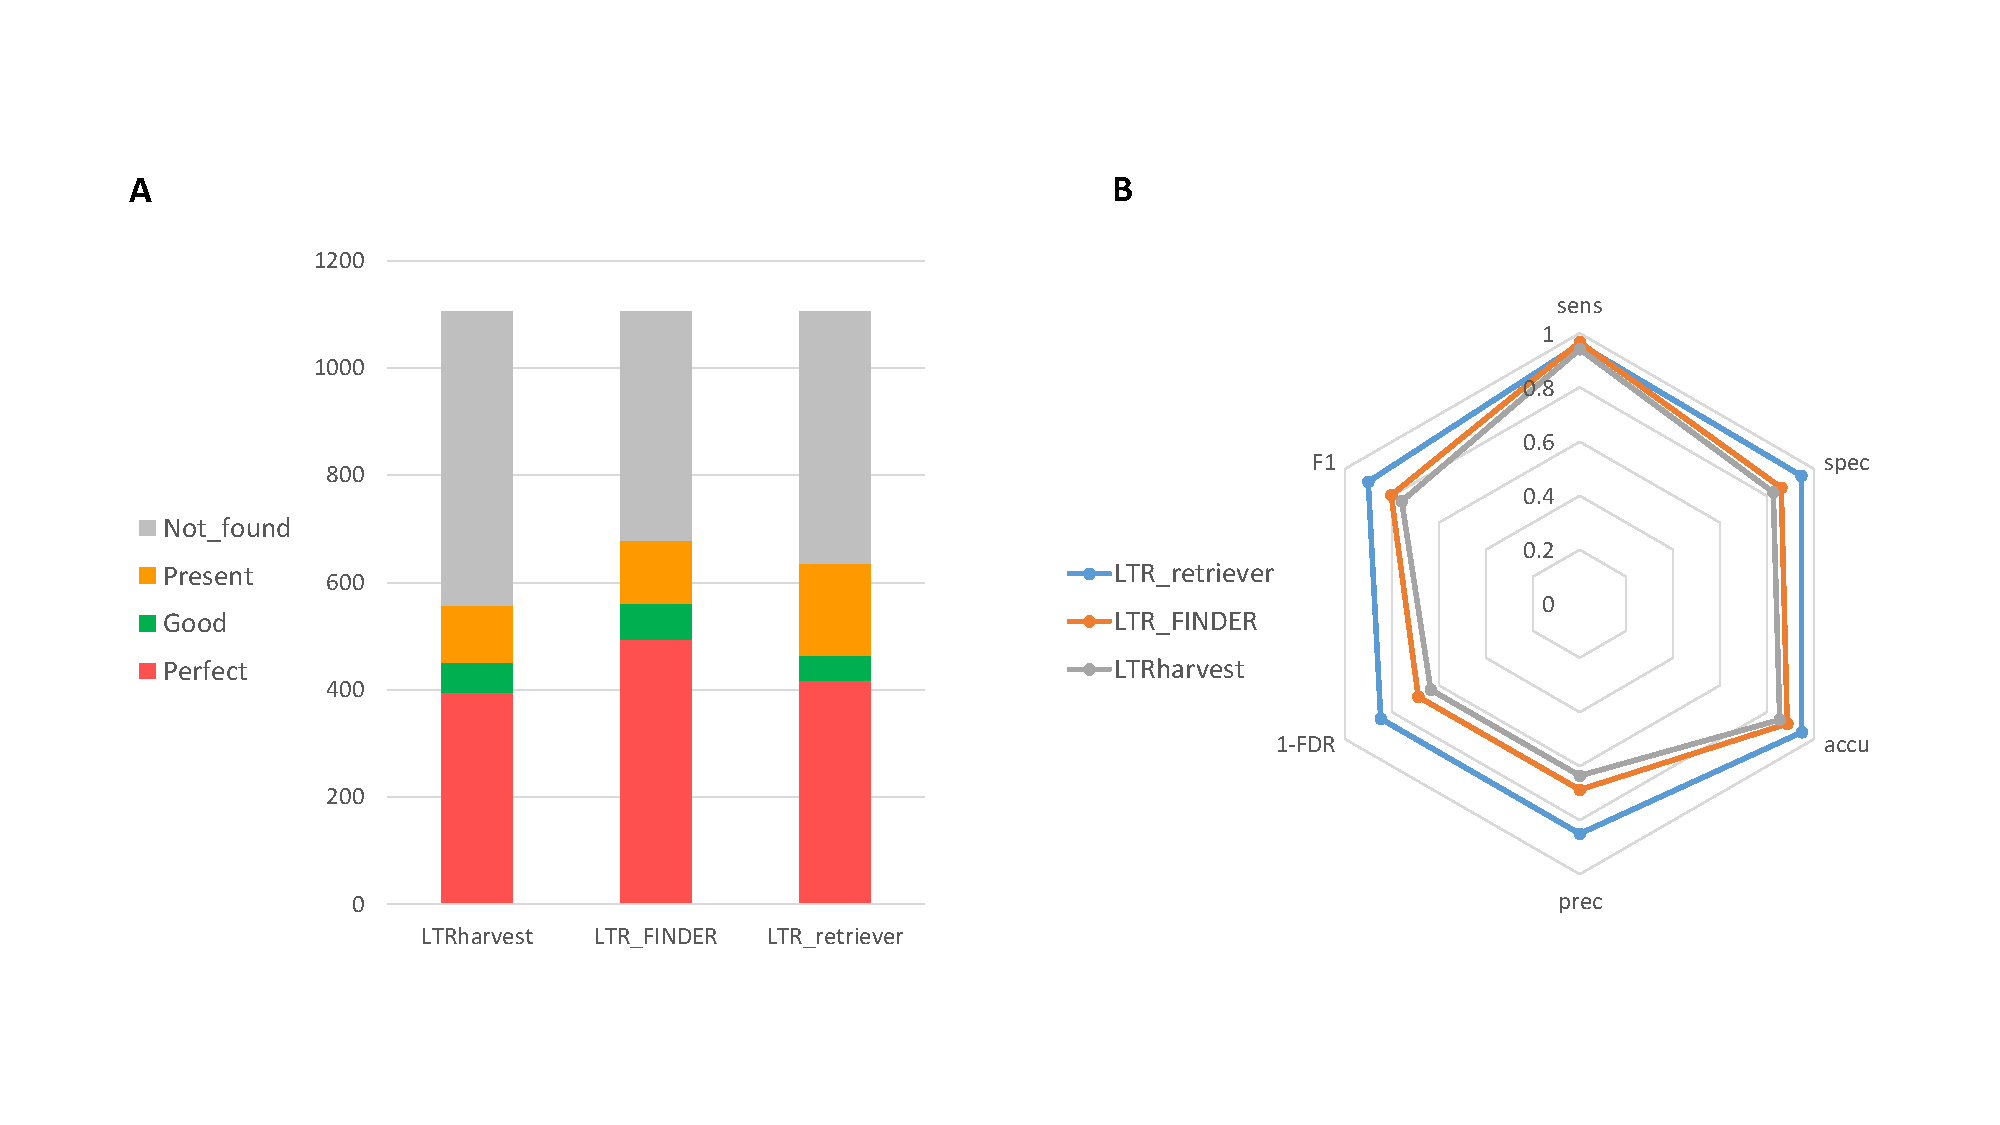
\includegraphics[width=1.0\textwidth]{figures/LTRResults.pdf}}
	\caption{Performance of LTR annotators. \textbf{a} the performance based on benckmarking method of RepeatModeler2 and \textbf{b} the performance based on benckmarking method of EDTA.}
	\label{fig:ltr_results}
\end{figure}

\subsection*{Performance comparison for LTR element detection}
Long terminal repeat retrotransposons (LTR-RTs) have a well-conserved structure and are prevalent in plant genomes. There are many tools dedicated to the \emph{de novo} identification of LTR-RTs, including MGEScan3\cite{lee2016mgescan}, GRF, LTR\_STRUC\cite{mccarthy2003ltr_struc}, LTR\_FINDER\cite{xu2007ltr_finder}, LTRharvest\cite{ellinghaus2008ltrharvest}, LtrDetector\cite{valencia2019ltrdetector}, and LTR\_retriever\cite{ou2018ltr_retriever}. It is worth noting that LTR\_retriever was designed as a stringent filtering method for raw results from other LTR tools and does not have its own search engine. We benchmarked the three best existing LTR \emph{de novo} identification tools, LTR\_FINDER, LTRharvest and LTR\_retriever (using the output of LTR\_FINDER and LTRharvest as input), and found that LTR\_FINDER and LTRharvest achieve higher sensitivity but lower precision, whereas LTR\_retriever significantly improves the precision while maintaining the same sensitivity (Fig. \ref{fig:ltr_results}b; Additional file 2: Table S2). The LTR\_retriever was integrated into a variety of TE detection pipelines, including EDTA and RepeatModeler2, and greatly improved the accuracy of their LTR identification. Although LTR\_retriever loses some \emph{Perfect} models (Fig. \ref{fig:ltr_results}a; Additional file 2: Table S2), it is still the best LTR identification method at present. Therefore, we integrated LTR\_retriever into HiTE.


\subsection*{Performance comparison for Non-LTR element detection}
Non-LTR retrotransposons include two types of TE, LINEs and SINEs\cite{zhao2016makes}. LINEs, which lack LTRs flanking both ends, can reach several kilobases in length. Although the presence of RT and nuclease in the pol ORF of LINEs seems to provide a confident basis for their identification, there is not a database dedicated to their curation. Worsely, the truncated 5$'$ ends, resulting from the premature termination of reverse transcription, make them difficult to discover. SINEs, on the other hand, are much shorter (80–500 bp)\cite{wicker2007unified}. They do not encode any reverse transcriptase protein and rely on other TEs to transition, especially LINEs\cite{dewannieux2003line}. The weak signals of non-LTR retrotransposons make them quite challenging to identify\cite{mao2017sine_scan}.

To accurately identify non-LTR retrotransposons, we have developed a homology-based TE searching module, named HiTE-Non-LTR. HiTE-Non-LTR extracts LINEs and SINEs consensus sequences from the Dfam library to form a non-LTR library, which is then used to search for confident candidate sequences based on the coarse boundaries of TE candidates output by the FMEA algorithm (see the \textbf{``Methods"} section). To benchmark the performance of the homology-based TE searching module, the non-LTR library is used to directly search candidates in the assembly genome as the competing evaluation, called Assembly-Non-LTR. Although HiTE-Non-LTR sacrificed a little sensitivity, it achieved nearly 100\% precision (Fig. \ref{fig:non_ltr_results}; Additional file 2: Table S2), which demonstrates the reliability of HiTE-Non-LTR.


\begin{figure}[h!]
	\centerline{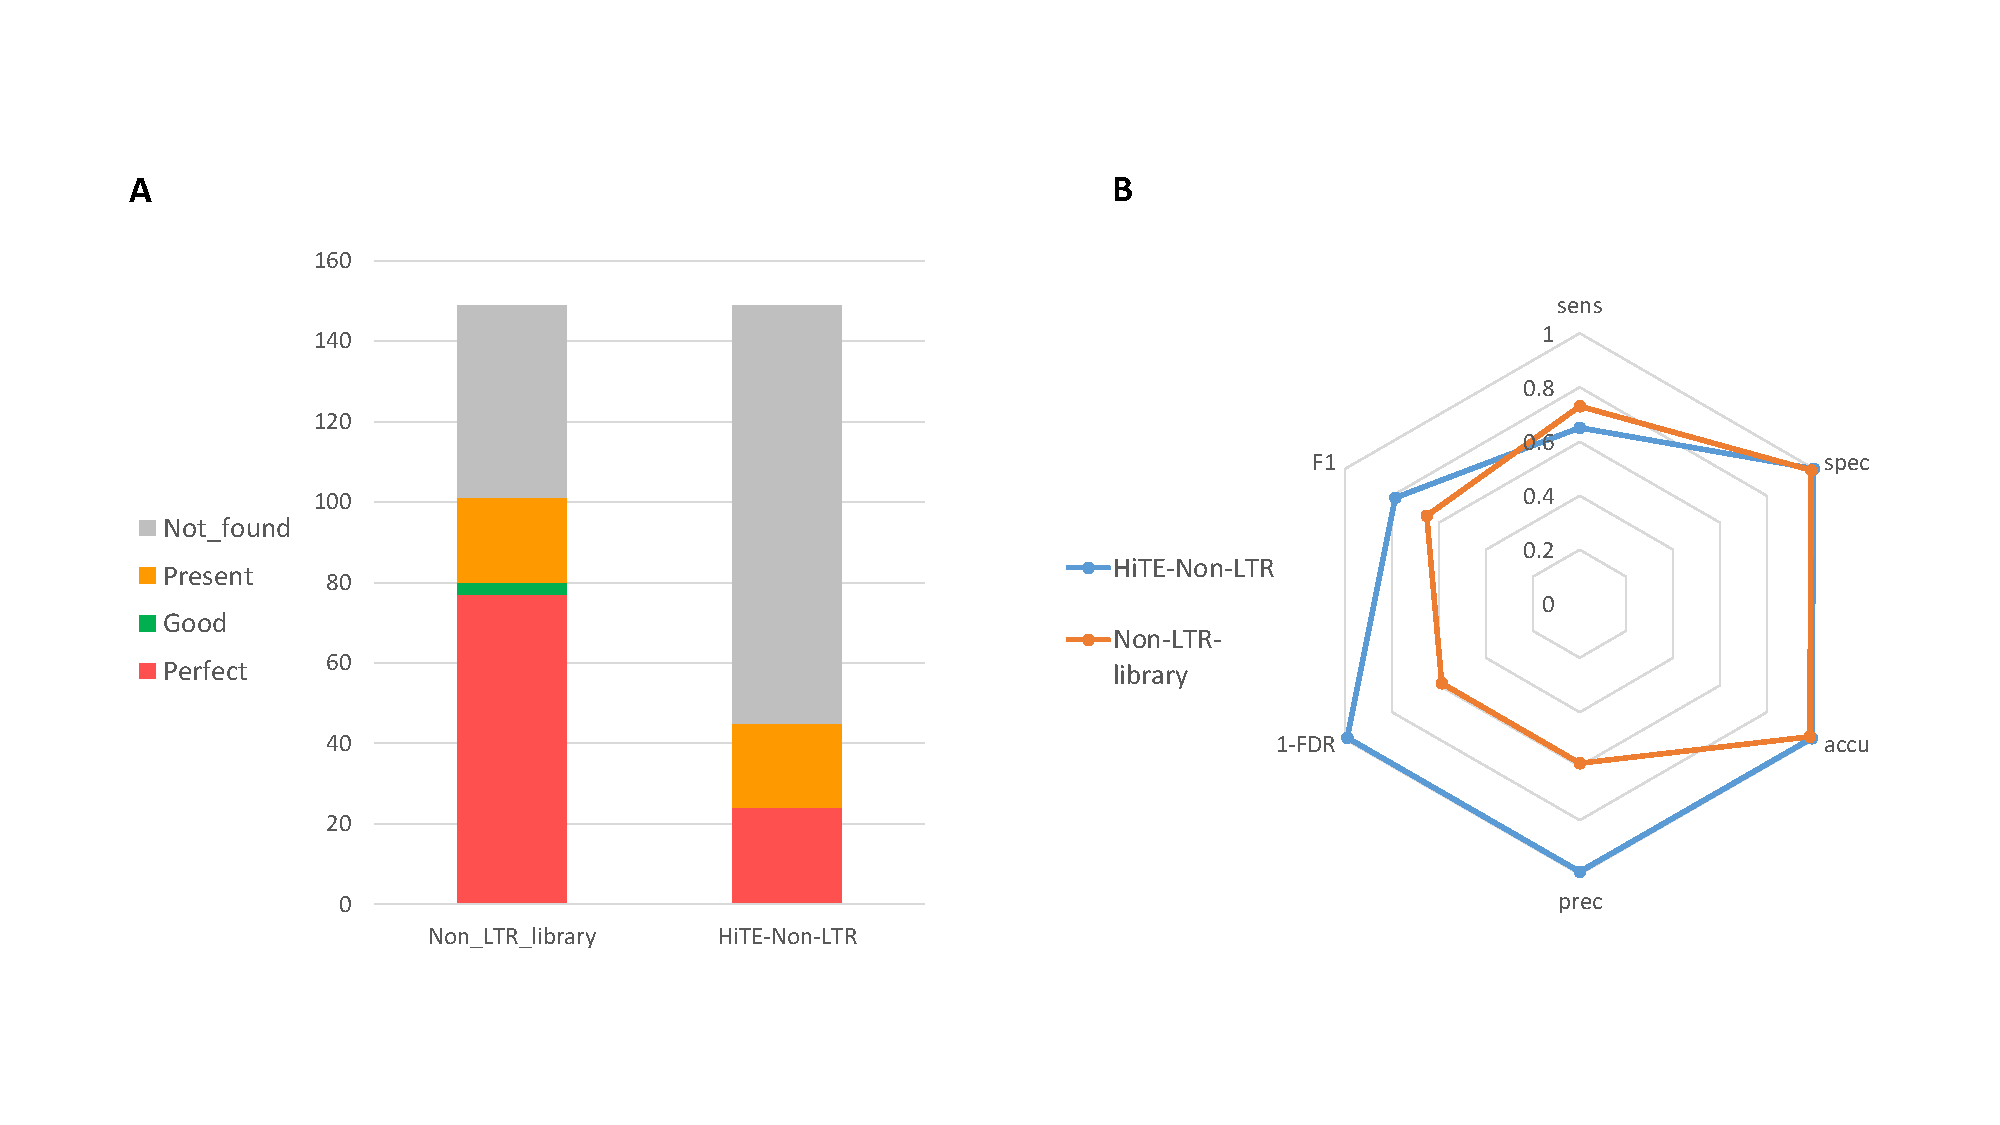
\includegraphics[width=1.0\textwidth]{figures/NonLTRResults.pdf}}
	\caption{Performance of Non-LTR annotators. \textbf{a} the performance based on benckmarking method of RepeatModeler2 and \textbf{b} the performance based on benckmarking method of EDTA.}
	\label{fig:non_ltr_results}
\end{figure}


\subsection*{Influence of parameter changes in HiTE}
To understand how the parameters in HiTE affect the results, we selected the four most important parameters for testing: k\_num, freq\_threshold, chunk\_size, and flanking\_len. The k\_num is the size of \emph{k}-mer, the freq\_threshold refers to the frequency threshold of \emph{k}-mer, the chunk\_size refers to cutting the genome into blocks of the same size, and the flanking\_len is used to extend the candidate TEs identified by FMEA to search for valid TSDs. Since these parameters have no effect on the results of LTR elements, which are discovered by LTR\_retriever, we chose C. briggsae as the test species, whose genome only contains a small number of LTR elements.

As shown in Fig. \ref{fig:param_results}a, the smallest k\_num (such as 11) will mark most parts of the genome as repeat regions, which cannot effectively distinguish TE from non-TE, resulting in low sensitivity and precision. Large k\_num will lose part of the true TE (lower sensitivity), but the sequences identified are more likely to be true TE (higher precision). Moderate k\_num (such as 31) achieves a balance between sensitivity and precision, the highest F1 value. When k\_num exceeds 41, we observe a significant drop in the number of \emph{Perfect} models. 
With the freq\_threshold increased, all metrics except precision decreased significantly, which indicates that the higher the frequency of \emph{k}-mer in the sequence, the more likely the sequence is to be a real TE (Fig. \ref{fig:param_results}b).
Genome slicing will result in the loss of some low-copy and scattered TEs, reducing the sensitivity of the results significantly. The smaller the cut, the more TEs will be lost (Fig. \ref{fig:param_results}c).
As shown in Fig. \ref{fig:param_results}d, when flanking\_len is set to 0, the number of sensitivity and \emph{Perfect} models is very low, which indicates that most of the TEs identified in the FMEA algorithm have coarse boundaries, while the real boundaries of most TEs can be included when flanking\_len is set to 10, suggesting that the error between the rough boundaries and the real boundaries is not significant. The metrics tend to be stable after flanking\_len is set to 40.


\begin{figure}[h!]
	\centerline{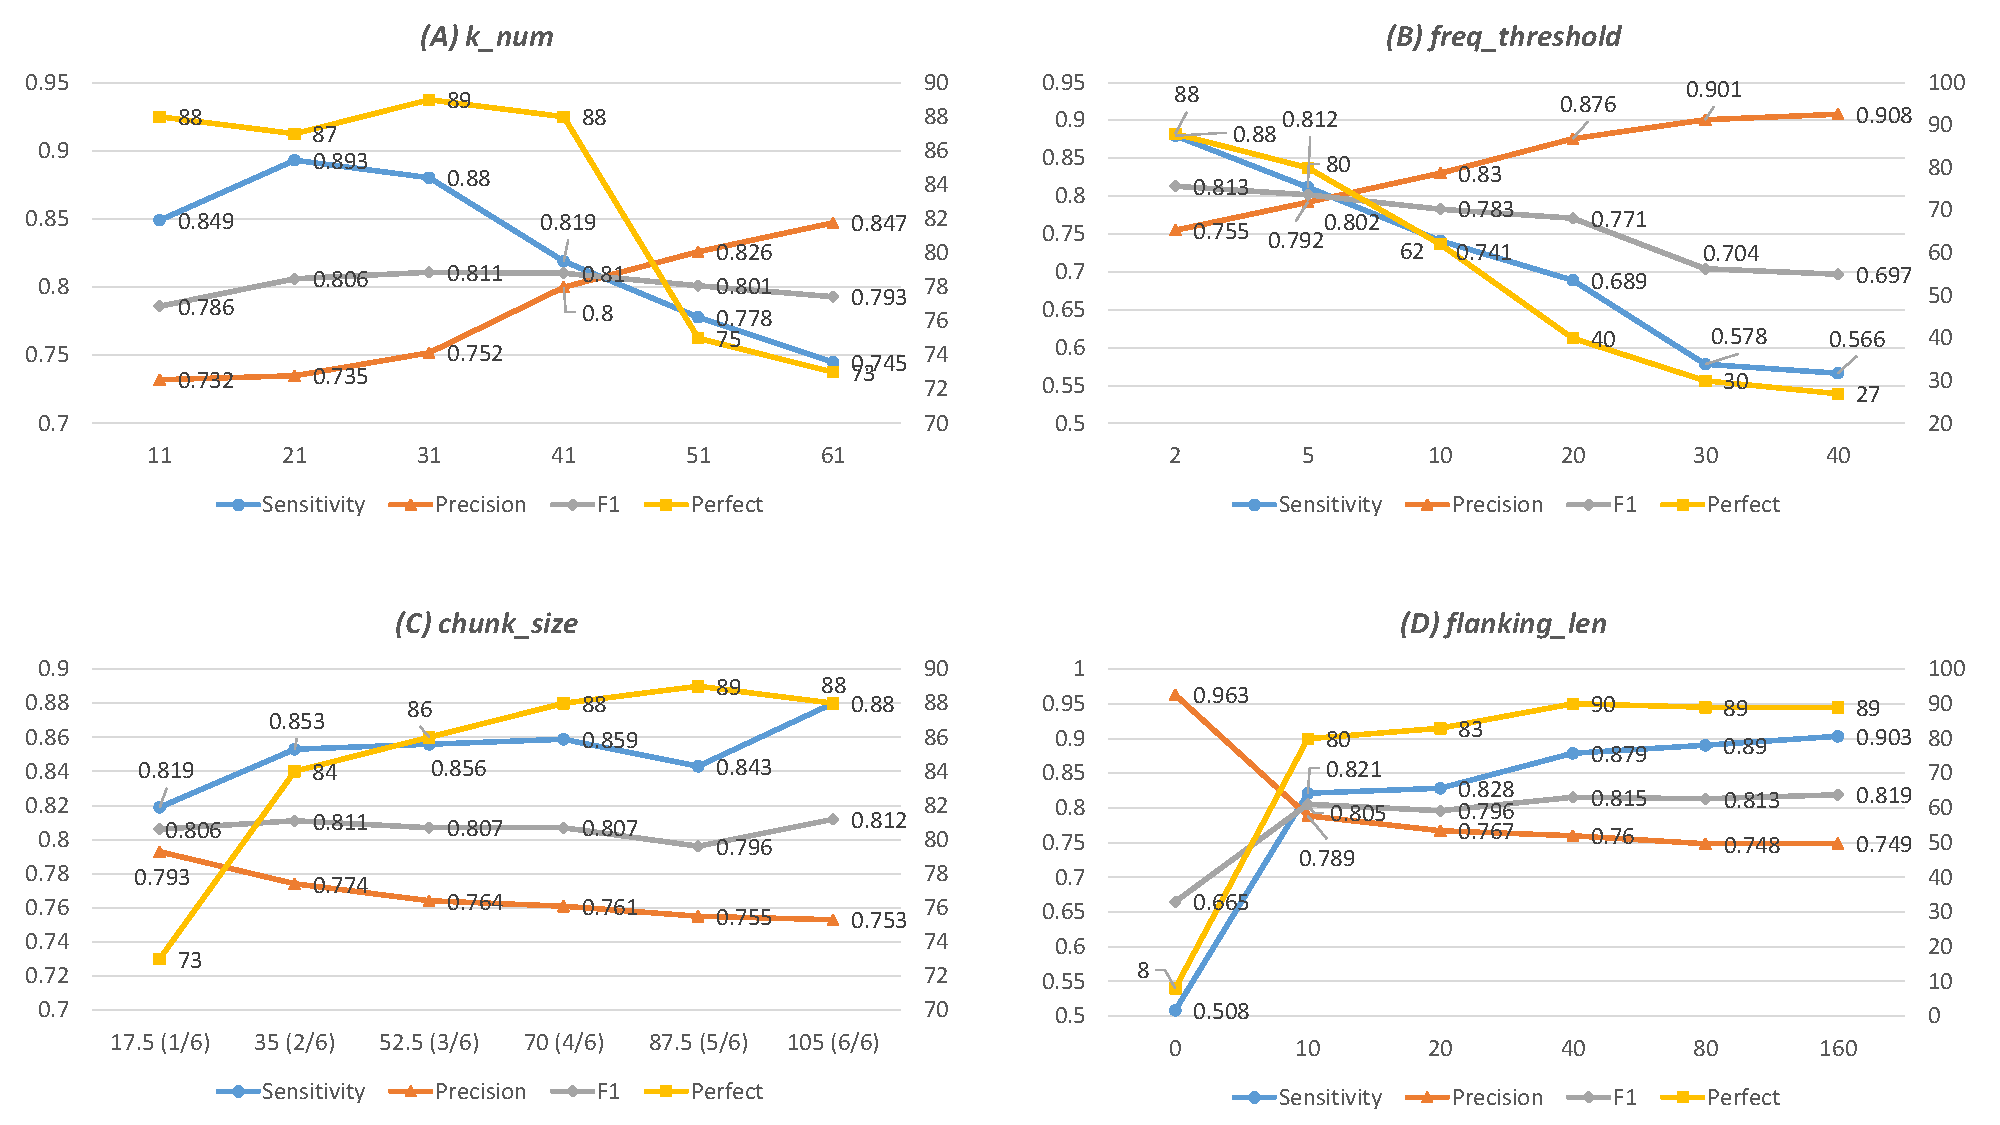
\includegraphics[width=1.0\textwidth]{figures/ParamResults.pdf}}
	\caption{Influence of parameter changes on results. \textbf{a} influence of k\_num parameter on results; \textbf{b} influence of freq\_threshold parameter on results; \textbf{c} influence of chunk\_size parameter on results; and \textbf{d} influence of flanking\_len parameter on results.}
	\label{fig:param_results}
\end{figure}

%\subsection*{Contribution of TEs to genome size}
%The amplification or contraction of transposable elements, affected by environmental stressors, is closely related to the genome size\cite{canapa2015transposons, zhang2019landscape}. LTR retrotransposons, especially the Ty3-gypsy elements, which are the major component in most plants, play an important role in the genome size variation across the Oryza genus\cite{ zuccolo2007transposable}.
%
%By applying HiTE to several common rice subspecies, Oryza sativa, Oryza rufipogon, and Oryza glaberrima, we observed that there was significant genome size variation among these rice genus, and the main source of genome size difference is the Gypsy transposon (Fig. \ref{fig:rice_diff}), as previously documented. The TE libraries of rice genomes are generated by HiTE using the default parameters. RepeatMasker is then used to generate the length coveage based on these TE libraries. 

%\begin{figure}[h!]
%	\centerline{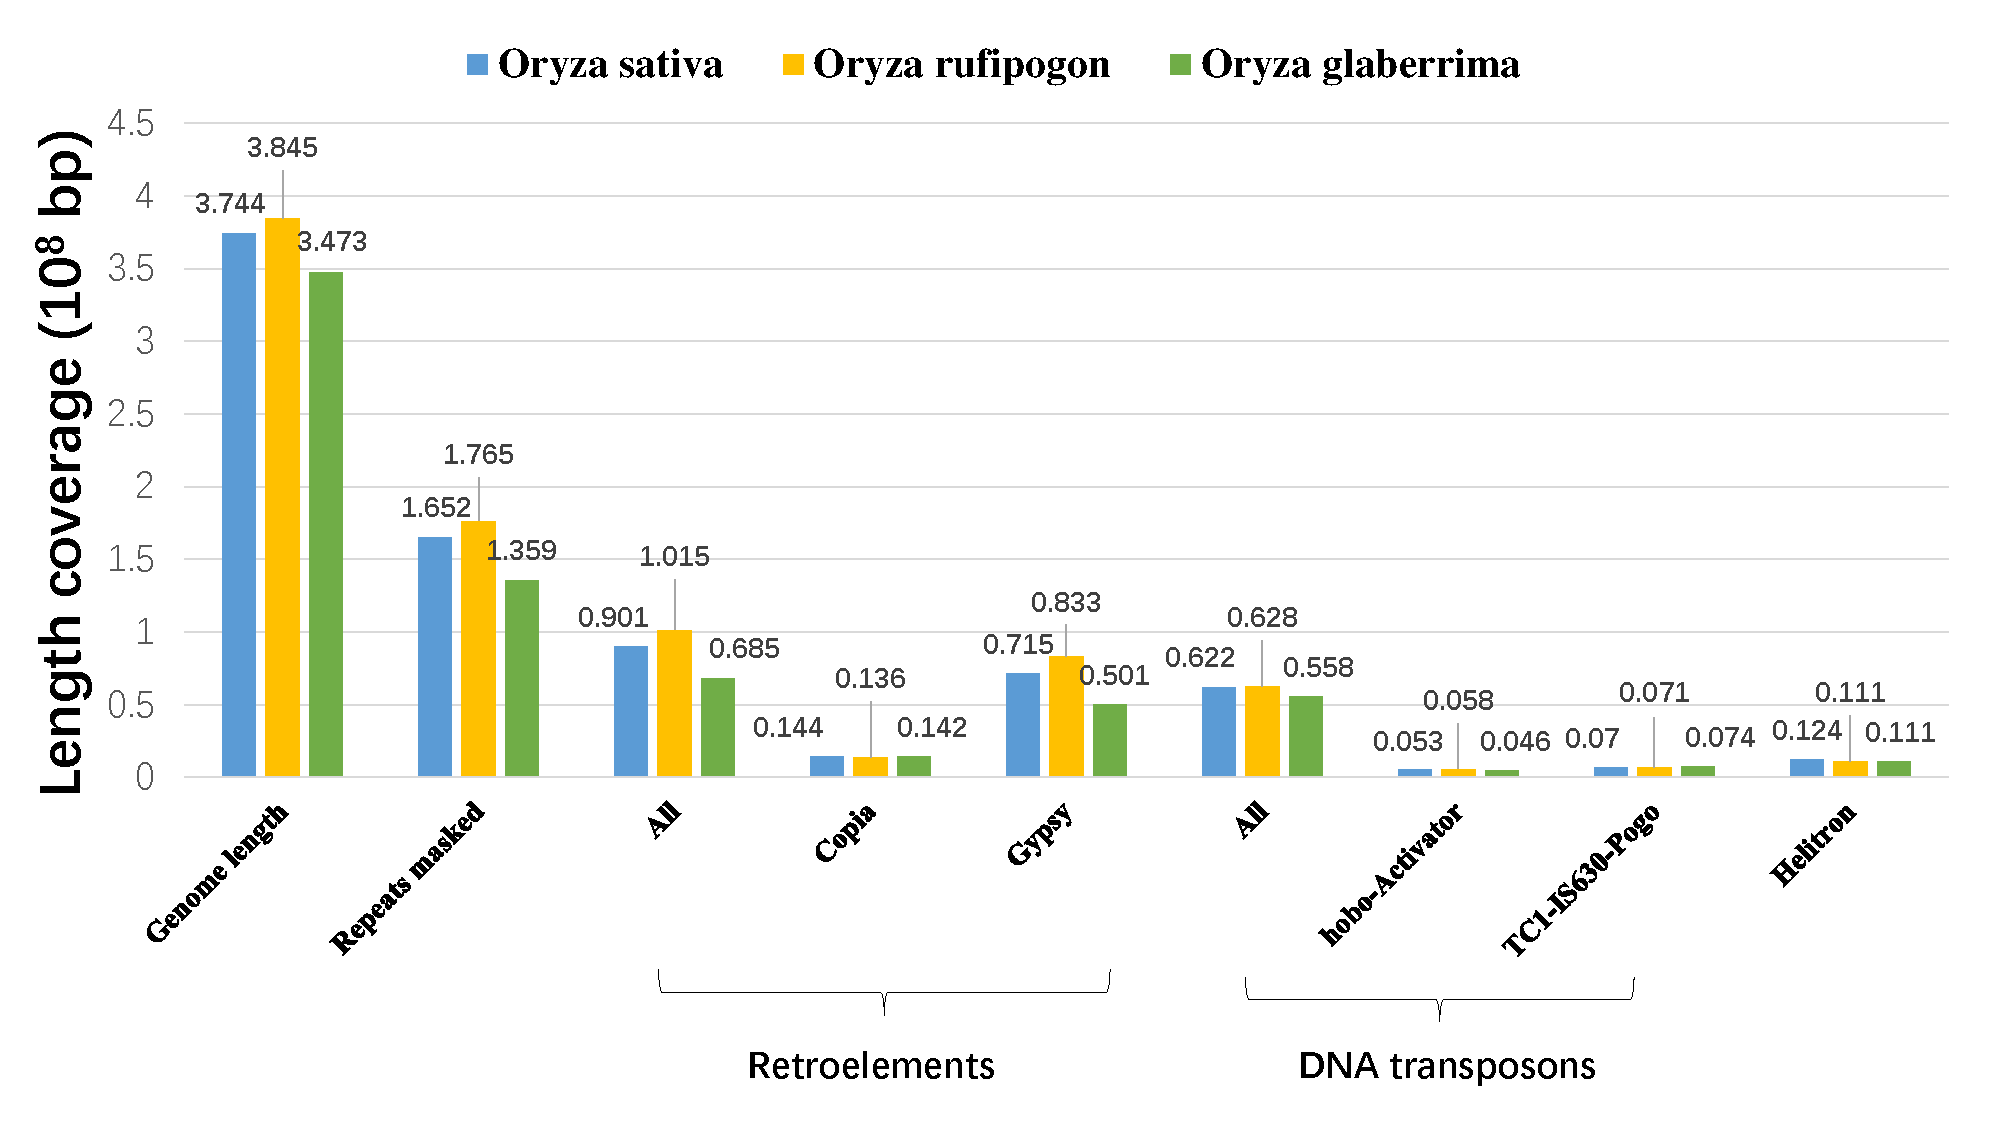
\includegraphics[width=1.0\textwidth]{figures/RiceDiff.pdf}}
%	\caption{The length coverage distribution of different types of transposons based on the analysis of rice genus.}
%	\label{fig:rice_diff}
%\end{figure}


\section*{Discussion}
%Thanks to decades of manual annotation results, we have obtained a highly reliable TE library for a limited number of species. 
With the development of third-generation (long-read) sequencing technology, repetitive regions in the genome can be crossed, which greatly improves the quality of genome assembly. While quantities of high-quality genome assemblies are being generated, an automated and high-precision TE annotation tool is urgently needed for these newly assembled genomes. To solve this problem, we have developed an ensemble method for high-precision TE annotation, known as HiTE, which has undergone extensive benchmarking on four model species. Compared with competing tools, HiTE achieved higher metrics and restored more gold standard sequences.

HiTE has the following four innovations compared to the existing tools: (i) Using repeated \emph{k}-mer coverage to reduce the amount of computation. The traditional tool, RepeatScout, uses the \emph{k}-mer seed expansion method to identify repeats, while HiTE uses low-frequency repeated \emph{k}-mer to discover candidate repeat areas, which can reduce the amount of subsequent calculation. For example, the alignment-based identification methods take the whole genome as input to obtain pairwise alignments, while HiTE reduces the whole genome into candidate repeats, which saves a lot of computing resources (Additional file 2: Table S3). (ii) Designing a fault-tolerant mapping expansion algorithm to restore intact TEs. Highly fragmented sequences are often generated due to divergent TE models or nested TEs, which result in the multi-segment alignment of a complete TE. Alignment-based identification methods, such as RECON, use the single linkage clustering algorithm to generate TE models based on overlapping subsequences, which may identify the same TE as multiple ``piles" without edges connected, resulting in multiple TE models and fragments. We have designed an alignment expansion method with fault tolerance that can cross the large gaps caused by insertion, deletion, and nested TE while retaining the complete TE structures. (iii) Defining the boundaries of TEs accurately. The TE library generated by automated identification methods still needs a lot of manual identification and repair\cite{storer2022methodologies}, mainly due to their inability to find the true boundaries of TEs. HiTE first used the self-alignment information to determine the coarse boundaries of TEs. Then, to accurately find the boundaries of TEs, both terminals of candidates are flanked to search for valid TSDs, which can greatly reduce the cost of manual identification and repair in the later period. (iv) Implementing a highly reliable filtering method. Weak structural characteristics of many TEs caused a flood of false positives, especially for DNA-TIR and Helitron transposons. We have designed a strict filtering method based on the following truth: once the boundaries are determined, the regions outside of the true TE instances should be close to the random sequences. Therefore, more than half of the candidate copies have homology outside the boundaries, indicating that these copies belong to a larger repeat, which is considered a false positive and should be filtered out.

%The identification of TEs requires intensive and sensitive sequence alignments, which is a computationally demanding task. HiTE uses k-mer coverage to reduce computation. Unlike the traditional k-mer-based seed expansion method, RepeatScout, HiTE uses low-frequency k-mer to determine candidate repeat areas, which reduces the number of sequence alignments and speeds up subsequent computation. 
%
%The TE-derived sequences in the genome accumulate variations over time, making their discovery and characterization challenging for the TE annotation methods. As time goes by, TEs are often accompanied by a large number of deletion and insertion variations when replicating and copying themselves. At the same time, their insertion sites on the genome are usually random, leading to complex sequence patterns of TE in the genome, such as nested TE structures, making accurate TE identification and annotation extremely difficult. It is easy for a complete TE sequence to generate multi-segment alignment due to the influence of divergence and nested TE during its evolution. The pairwise alignment-based identification methods, such as RECON, may identify a complete TE model as multiple pieces without edges connected and generate multiple TE models using the single linkage clustering algorithm. We have designed an alignment expansion method with fault tolerance that can easily cross the large gaps caused by insertion, deletion, and nested TE and retain the complete TE structure as much as possible.
%
%Although it is important to accurately identify the structures and boundaries of TEs, repeatedness-based methods, such as RepeatModeler\cite{Smit2008repeatmodeler}, always obtain uncertain boundaries, and intensive manual repairs are required to enable them to be saved in the cured library\cite{storer2022methodologies}. HiTE first used the sensitive sequence alignment information to determine the coarse boundaries of TEs based on the fault-tolerant alignment expansion method. Then, the coarse boundaries are flanked to search for valid TSD and terminal motifs. Finally, a reliable false-positive filtering method is developed to get confident TEs with multiple intact copies and clear TE boundaries.

While HiTE can achieve high-precision TE identification and annotation, we do observe some losses of real TIR elements in Repbase, which are mainly caused by the following reasons:
(i) Repbase contains many single-copy sequences, even zero-copy sequences. For zero-copy sequences, it is possible that these sequences come from multiple genomes of the same species, such as different types of rice, which we cannot identify based on a single genome, or they are from degraded nested TEs without other full-length copies in the genome. At the same time, to ensure the high reliability of identified transposons, single-copy TEs, which require high homology with known transposons or TE proteins to identify, are also filtered out. Our method, such as the TIR identification module, needs at least two full-length copies to determine a true transposon, and most of the single-copy and zero-copy sequences are left out.
(ii) Some transposons have highly divergent terminals or TSDs. Highly divergent TIRs (identity less than 0.7) and the TEs with accidental sequence homology outside the boundaries, which is similar to many false positive patterns, are filtered out. We discover some lost real TIR elements by manually inspecting the results of FMEA, mainly for highly divergent TIRs and TSDs, which further proves the effectiveness of the FMEA algorithm. At the same time, a more accurate and comprehensive filtering method helps to find more real TIR elements.
%To achieve high-precision identification, we identify LTR and TIR elements by TSDs, and TEs with significant divergent TSDs are filtered out.

The identification of TEs with weak structural characteristics, such as Helitron and non-LTR elements, is very challenging. Although we have greatly improved the identification performance of Helitrons, there is still potential for improvement. For example, a more comprehensive hairpin loop pattern will significantly improve the sensitivity. To date, there is no structure-based method to identify LINEs due to the truncated 5$'$ ends of LINEs. A few tools designed for the identification of SINEs, which suffer from the high false positives and low sensitivity. To achieve high-precision non-LTR element annotation, we developed a homology-based TE searching method, which improves precision by nearly 100\%, while the structure-based identification methods of LINEs are still needed, which is also the direction of our future efforts.

\section*{Conclusions}
The rapid development of sequencing technologies is producing more reliable genome assemblies, which gives a bright future to comprehensive annotation of TEs. However, the TE libraries generated by inaccurate TE identification tools will contain many errors, which will be propagated during the whole-genome annotation process. HiTE makes full use of the strengths and weaknesses of existing methods, which can comprehensively and accurately identify and annotate TEs in the genome assembly. By benchmarking on four model species with different TE landscapes, we prove that HiTE can achieve higher accuracy and restore more gold standard TE models, which can be fully applied to any new sequencing genome assembly.

\section*{Methods}

\subsection*{Kmer-Based De Novo TE Searching}
The majority of \emph{de novo} identification methods, such as RECON, are based on pairwise alignments to identify repeats. However, pairwise alignments of genomes will consume a lot of computing resources. To solve this problem, we designed the RepeatMasking method, which can reduce the search scope of the whole genome into marked candidate repeats.

The discovery of the raw repeat region is based on the following observation: if there are two repeat sequences, regardless of the variations, the \emph{k}-mers composed of these two repeat sequences are also repeated. Therefore, we can in turn identify candidate repeat sequences by covering the repeated \emph{k}-mers in the genome (Fig. \ref{fig:framework}k; Additional file 1: AlgorithmS1). It is worth noting that due to the variations between the two repeat sequences, the continuous repeat regions may break into small pieces due to a lack of duplicate \emph{k}-mers. We try to skip these small gaps and connect the scattered repeat areas. Furthermore, the fake \emph{k}-mers may falsely connect multiple repeat regions together to form a larger repeat region, which can be degraded by the fault-tolerant mapping expansion algorithm.

%\begin{figure}[h!]
%	\centerline{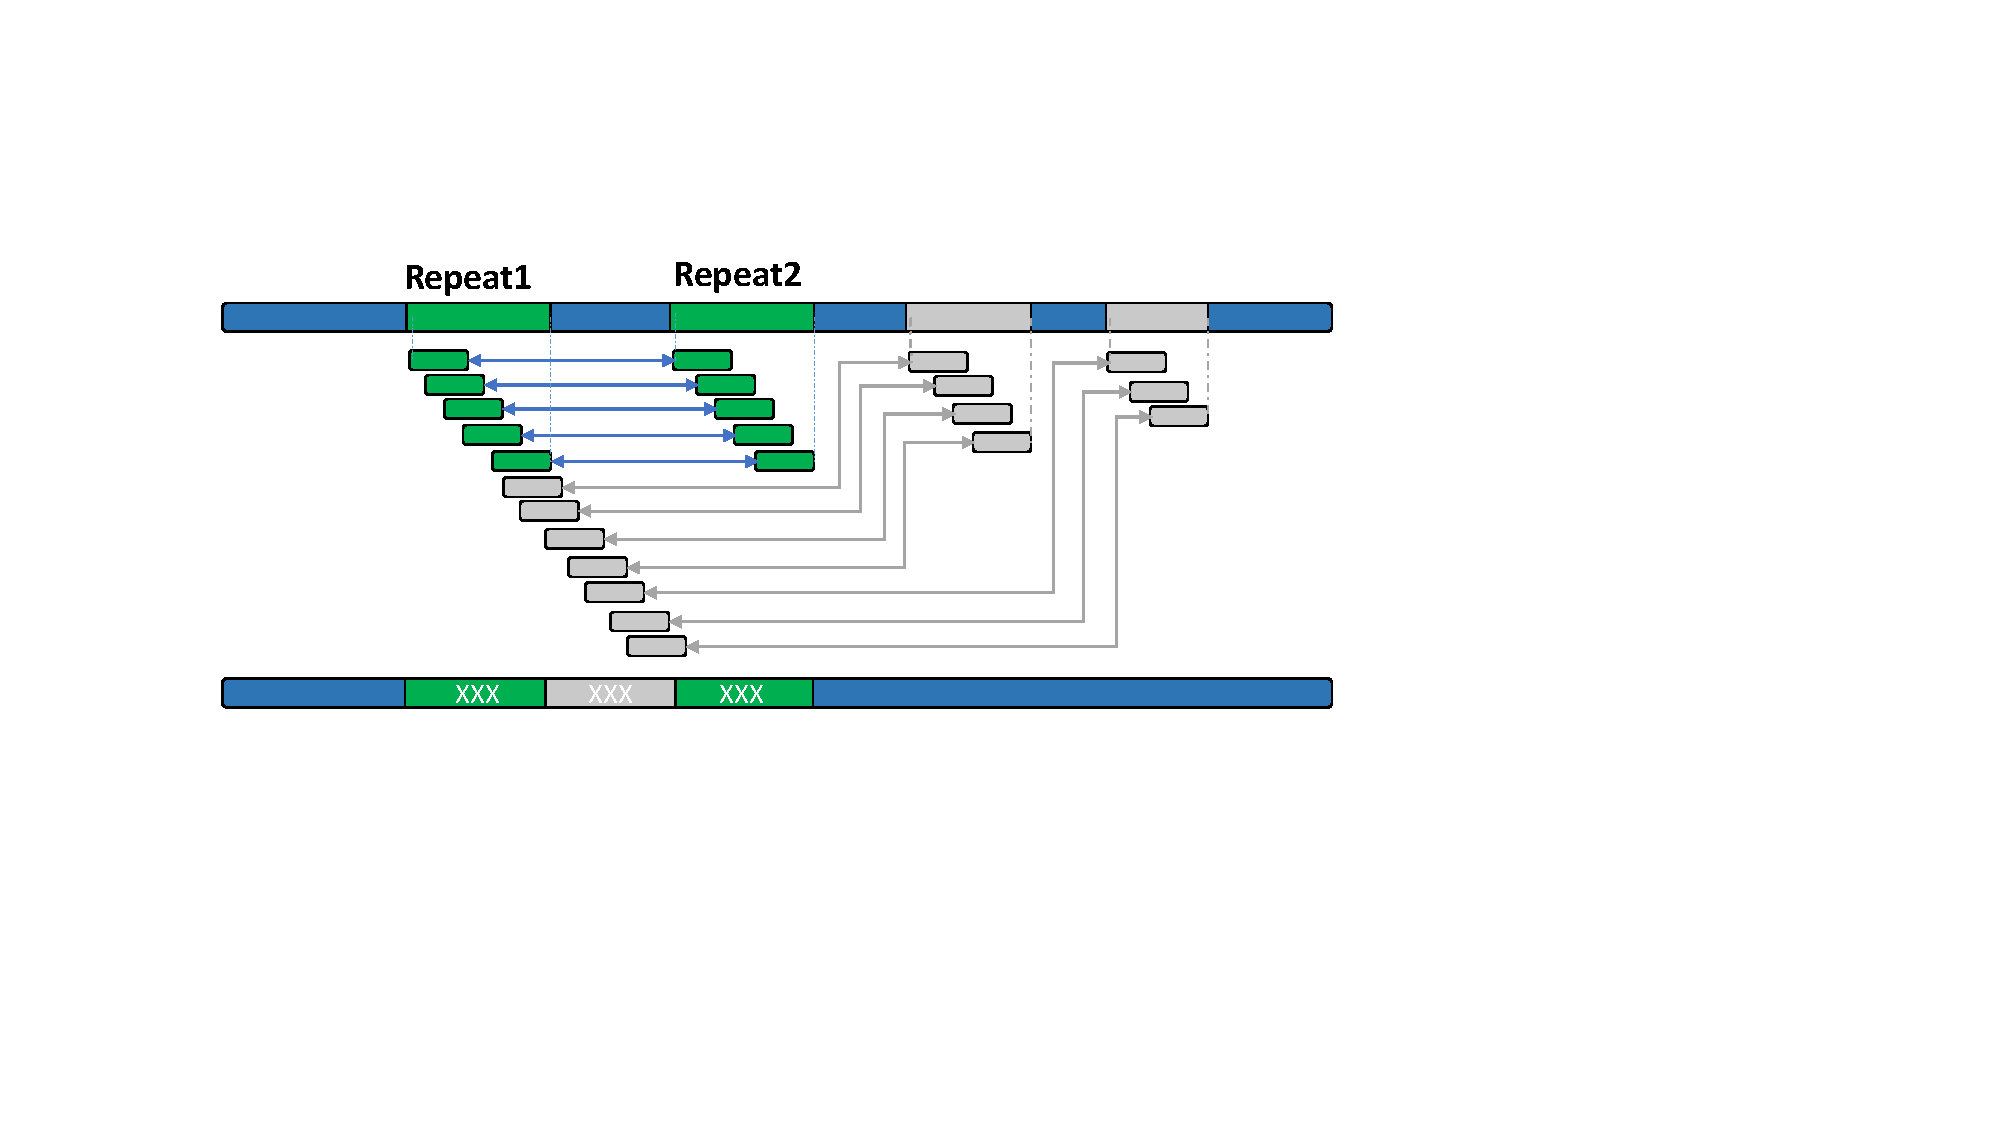
\includegraphics[width=1.0\textwidth]{figures/RepeatMasking.pdf}}
%	\caption{The illustration of RepeatMasking. The long blue bar represents the genome, and the green box on the genome represents two repeat sequences, Repeat1 and Repeat2. The small green box below represents the k-mers of the real repeat sequence (the frequency of occurrence is at least 2 times), and the small grey box represents the confused k-mers, that is, although the frequency is more than 2 times, it does not belong to the real repeat sequence. The area marked with an X below is the candidate repeat area identified by the program.}
%	\label{fig:repeatmasking}
%\end{figure}

%Algorithm \ref{RepeatMasking} describes the RepeatMasking algorithm, where \emph{G} is genome assembly, \emph{k} is the size of the \emph{k}-mer, \emph{L} is the length of divided genome segments, and \emph{g} is the maximum length of the gap between adjacent repeat regions; \emph{R} is the set of candidate repeat regions; The buildRTable(·) function is used to construct the hash table of repeated \emph{k}-mers, the cutSegments(·) function is used to divide the whole genome into genome segments, the cutKmers(·) function cuts the genome segments into \emph{k}-mers, the queryRtable(·) function is used to judge whether \emph{k}-mers are repeated by querying the repeated \emph{k}-mers hash table, and the maskSequence(·) is a function to mark repeated sequences, The skipGaps(·) function connects adjacent repeat sequences to skip small gaps, while the extractRepeats(·) function is used to extract candidate repeat sequences from masked sequences.
%
%To analyze the time complexity of RepeatMasking, we noticed that DSK is a highly efficient tool that can process a mammalian genome in a few minutes, so the buildRTable(·) function actually takes very little time. The cutSegments(·) function divides the whole genome assembly into $N/L$ segments, where N=length(G). Both cutKmers(·) and maskSequence(·) have O (L) time complexity, while queryRtable(·) has O (1) time complexity. The total time complexity of algorithm \ref{RepeatMasking} is O(N·L), which is a function of \emph{N} and \emph{L}. In general, \emph{L} is set as a fixed constant. In addition, since we use multiprocessing technology to accelerate the program, the running time of RepeatMasking can be reduced to \emph{t} times the original, where \emph{t} is the number of processes. Therefore, this algorithm has high efficiency in actual application.
%\begin{algorithm}  
%	\caption{RepeatMasking}\label{RepeatMasking}
%	\begin{algorithmic}[1]  
%		\Require 
%		G, k, L, g
%		\Ensure 
%		R
%		\Function {RepeatMasking}{G, k, L, g}
%		\State $H \gets buildRTable(G, k)$
%		\State $S \gets cutSegments(G, L)$
%		\State $R \gets \emptyset$
%		\For{$i = 0 \to length(S)$}
%		\State $s \gets S[i]$
%		\State $P \gets cutKmers(s, k)$
%		
%		\For{$j = 0 \to length(P)$}
%		\State $p \gets P[j]$
%		\State $isRepeated \gets queryRtable(H, p.kmer)$
%		
%		\If {$isRepeated$}
%		\State $s^{\prime} \gets maskSequence(s, p.start, p.end)$          
%		\EndIf
%		
%		\EndFor 
%		
%		\State $s^{\prime \prime} \gets skipGaps(s^{\prime}, g)$ 
%		\State $r \gets extractRepeats(s^{\prime \prime})$ 
%		\State $R \gets R \cup r$ 
%		
%		\EndFor             
%		\EndFunction
%	\end{algorithmic}  
%\end{algorithm}

\subsection*{Fault-tolerant Mapping Expansion Algorithm}
The alignment-based method can identify more complete and biologically meaningful TE sequences. At the same time, due to the serious divergence between TE instances and the existence of a large number of insertions and deletions, we must consider fault tolerance when identifying TEs. Traditional alignment-based methods may divide a single TE instance into multiple fragments that negatively affect the identification and classification of complete TE families. Therefore, we designed a fault-tolerant mapping expansion algorithm (FMEA) that can span a large gap.

The algorithm first performs self-alignment on the raw repeats masked by RepeatMasking (Fig. \ref{fig:framework}l; Additional File 1). For each query sequence, adjacent alignments are gathered based on their alignment positions on the subject and then sorted ascending based on query alignment positions. If the next alignment is still in the adjacent area of the previous alignment, expand the previous alignment until it cannot be expanded. Each query will obtain multiple extension sequences, and the redundant sequences are removed. The longest sequence with more than two copies represents an intact repeat.

%\begin{figure}[h!]
%	\centerline{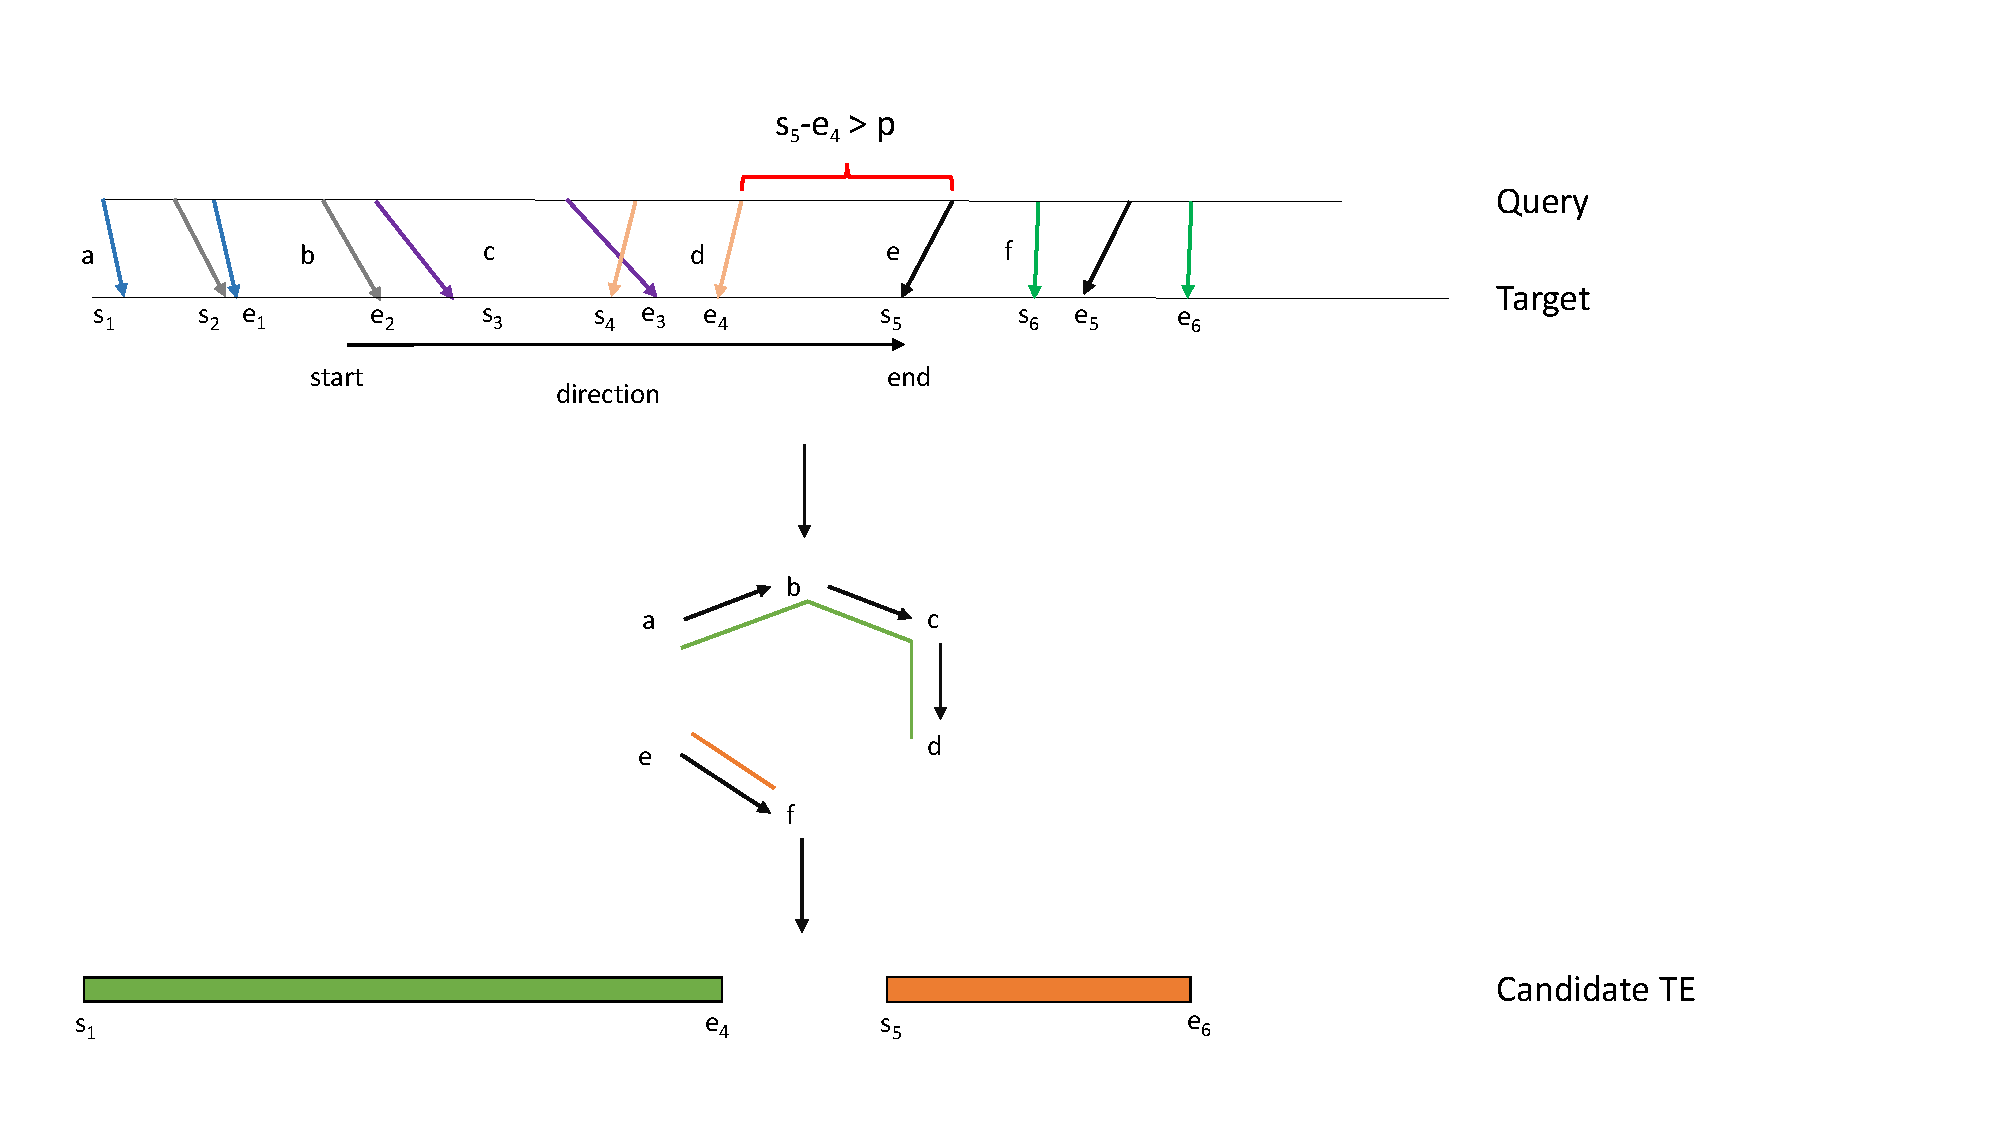
\includegraphics[width=1.0\textwidth]{figures/FMEA.pdf}}
%	\caption{The illustration of the fault-tolerant mapping expansion algorithm.}
%	\label{fig:fmea}
%\end{figure}

%\subsubsection*{Example description}
%Due to the existence of insertion, deletion, and multiple TE sequences, multiple subsequence alignments will be generated in the candidate repeat area, as shown in Fig. \ref{fig:framework}(k): a, b, c, d, e, f. The above algorithm can be simply described as the following process:
%
%1. We start by setting an extended threshold value p, then sort the alignments by starting and ending positions.
%
%2. For each alignment, judge whether its adjacent alignment can expand the sequence length. For example, the first is the alignment of subsequence a, whose starting and ending positions are s1 and e1; the starting and ending positions of subsequence b are s2 and e2. Since e2 $\textgreater $e1 and s2-e1$\textless$p, it means that adding b can expand the length of the current subsequence, so we connect the subsequences a and b. Similarly, connect subsequences c and d. However, since s5-e4$\textgreater $p, it indicates that the subsequence e is too far from sequence d to cross the gap in the middle, which should belong to two different TE instances. The TE instances in the above example are TE sequence 1 (starting s1, terminating e4) composed of subsequences a, b, c and d and TE sequence 2 (starting s5, terminating e6), corresponding to subsequences e and f.
%
%3. Since the query will be aligned to multiple different targets, we will get a set with overlapped sequences. We think that two sequences in the overlapped set have more than 95\% overlap, and they are considered to be copies of each other. A representative sequence is used to represent all copies with overlap, and the boundary of the representative sequence is updated to include all copy sequences. Finally, we get a collection of non-overlapping repeats.

\subsection*{Structural-Based TE Searching}
TEs have certain structural characteristics, such as LTR and TIR characteristics at both ends of LTR and TIR elements. In addition, when TE is inserted into the genome, it is usually accompanied by DNA double-strand breaks, whose repair results in the formation of two short target site duplications (TSDs; usually 2–11 bp) at the integration site. The size of the TSDs can be used as a diagnostic feature for TE identification and classification. Structural-based TE searching methods can discover structurally intact TEs by identifying these TE superfamily-specific structural features. %We describe the structural characteristics of three main types of TE and refer to the review for more TE structural characteristics\cite{wicker2007unified}.

LTR-RTs typically have long direct repeat sequences (85 to 5000 bp), 2-bp palindromic motifs, 5$'$-TG..CA-3$'$ at both ends, and 4-6 bp TSDs flanked. The strong structural features of LTRs allow us to identify them directly based on the genome assembly. At present, there are some mature tools that can accurately identify TSDs and LTRs, such as LTR\_Finder, LTRharvest, and LTR\_retriever. We use LTR\_harvest and the parallel version of LTR\_Finder\cite{ou2019ltr_finder_parallel, xu2007ltr_finder} to identify candidate sequences with LTR structures in the genome, and LTR\_retriever is used as a stringent filtering method for the raw results from the other two tools. LTR\_Finder uses the default parameters, and LTR\_harvest uses the parameter ``-seed 20 -minlenltr 100 -maxlenltr 7000 -similar 85 -motif TGCA -mintsd 4 -maxtsd 6 -vic 10" (Additional file 2: Table S4).  Finally, false positives are filtered out by homology outside the boundaries of copies (see Section \textbf{Filtering false positives}).

TIR elements have terminal inverted repeat sequences (TIRs, usually a few bp to hundreds of bp) and conserved motif characteristics of some specific superfamilies. For example, DTC (CACTA) starts and ends with the conserved sequence 5$'$-CACTA...TAGTG-3$'$; DTT and DTH transposons have conserved TSDs of ``TA" and ``TNN", respectively. However, TIR elements are challenging to identify due to their short terminals. Most TIR identification tools still suffer from a large number of false positives. To discover the intact TIR elements, we first use the RepeatMasking and FEMA algorithms to determine the coarse boundaries of candidate TEs. Then, the coarse boundaries are extended by a certain length to search for all legal TSDs (Fig. \ref{fig:framework}n). We identify the identical TSDs at most a 1 bp mismatch to reduce false positives. Following that, we use the itrsearch tool included in TE Finder 2.30 (a part of the REPET\cite{quesneville2010repet} package) with the parameter ``-i 0.7 - l 5" to search TIRs (Additional file 2: Table S4), and the sequences with TIRs and TSDs closest to the coarse boundaries are chosen as the candidate TIRs. Finally, we will determine whether the candidate TIR elements identified are true transposons using the filtering method. 

Helitron element replicates through the rolling circle mechanism. When replicating, only the single strand of DNA is broken, and no TSD is generated. Helitron element has a 5$'$-TC...-CTRR-3$'$ conserved structure (R refers to purine, A or G), and there is a short hairpin structure about 10 bp upstream of the 3$'$ end. All Helitrons previously identified in plants, fungi, and mammals have been characterized by precise transitions into host AT target sites\cite{kapitonov2007helitrons}. The weak structural signals of Helitrons make the identification of these elements particularly challenging. The identification of Helitrons in HiTE is still based on the candidate TEs with coarse boundaries generated by the RepeatMasking and FEMA algorithms. EAHelitron\cite{hu2019helitron} is then used to identify candidate sequences with Helitron structure. Finally, the filtering method is used to filter out false positives.

%\begin{figure}[h!]
%	\centerline{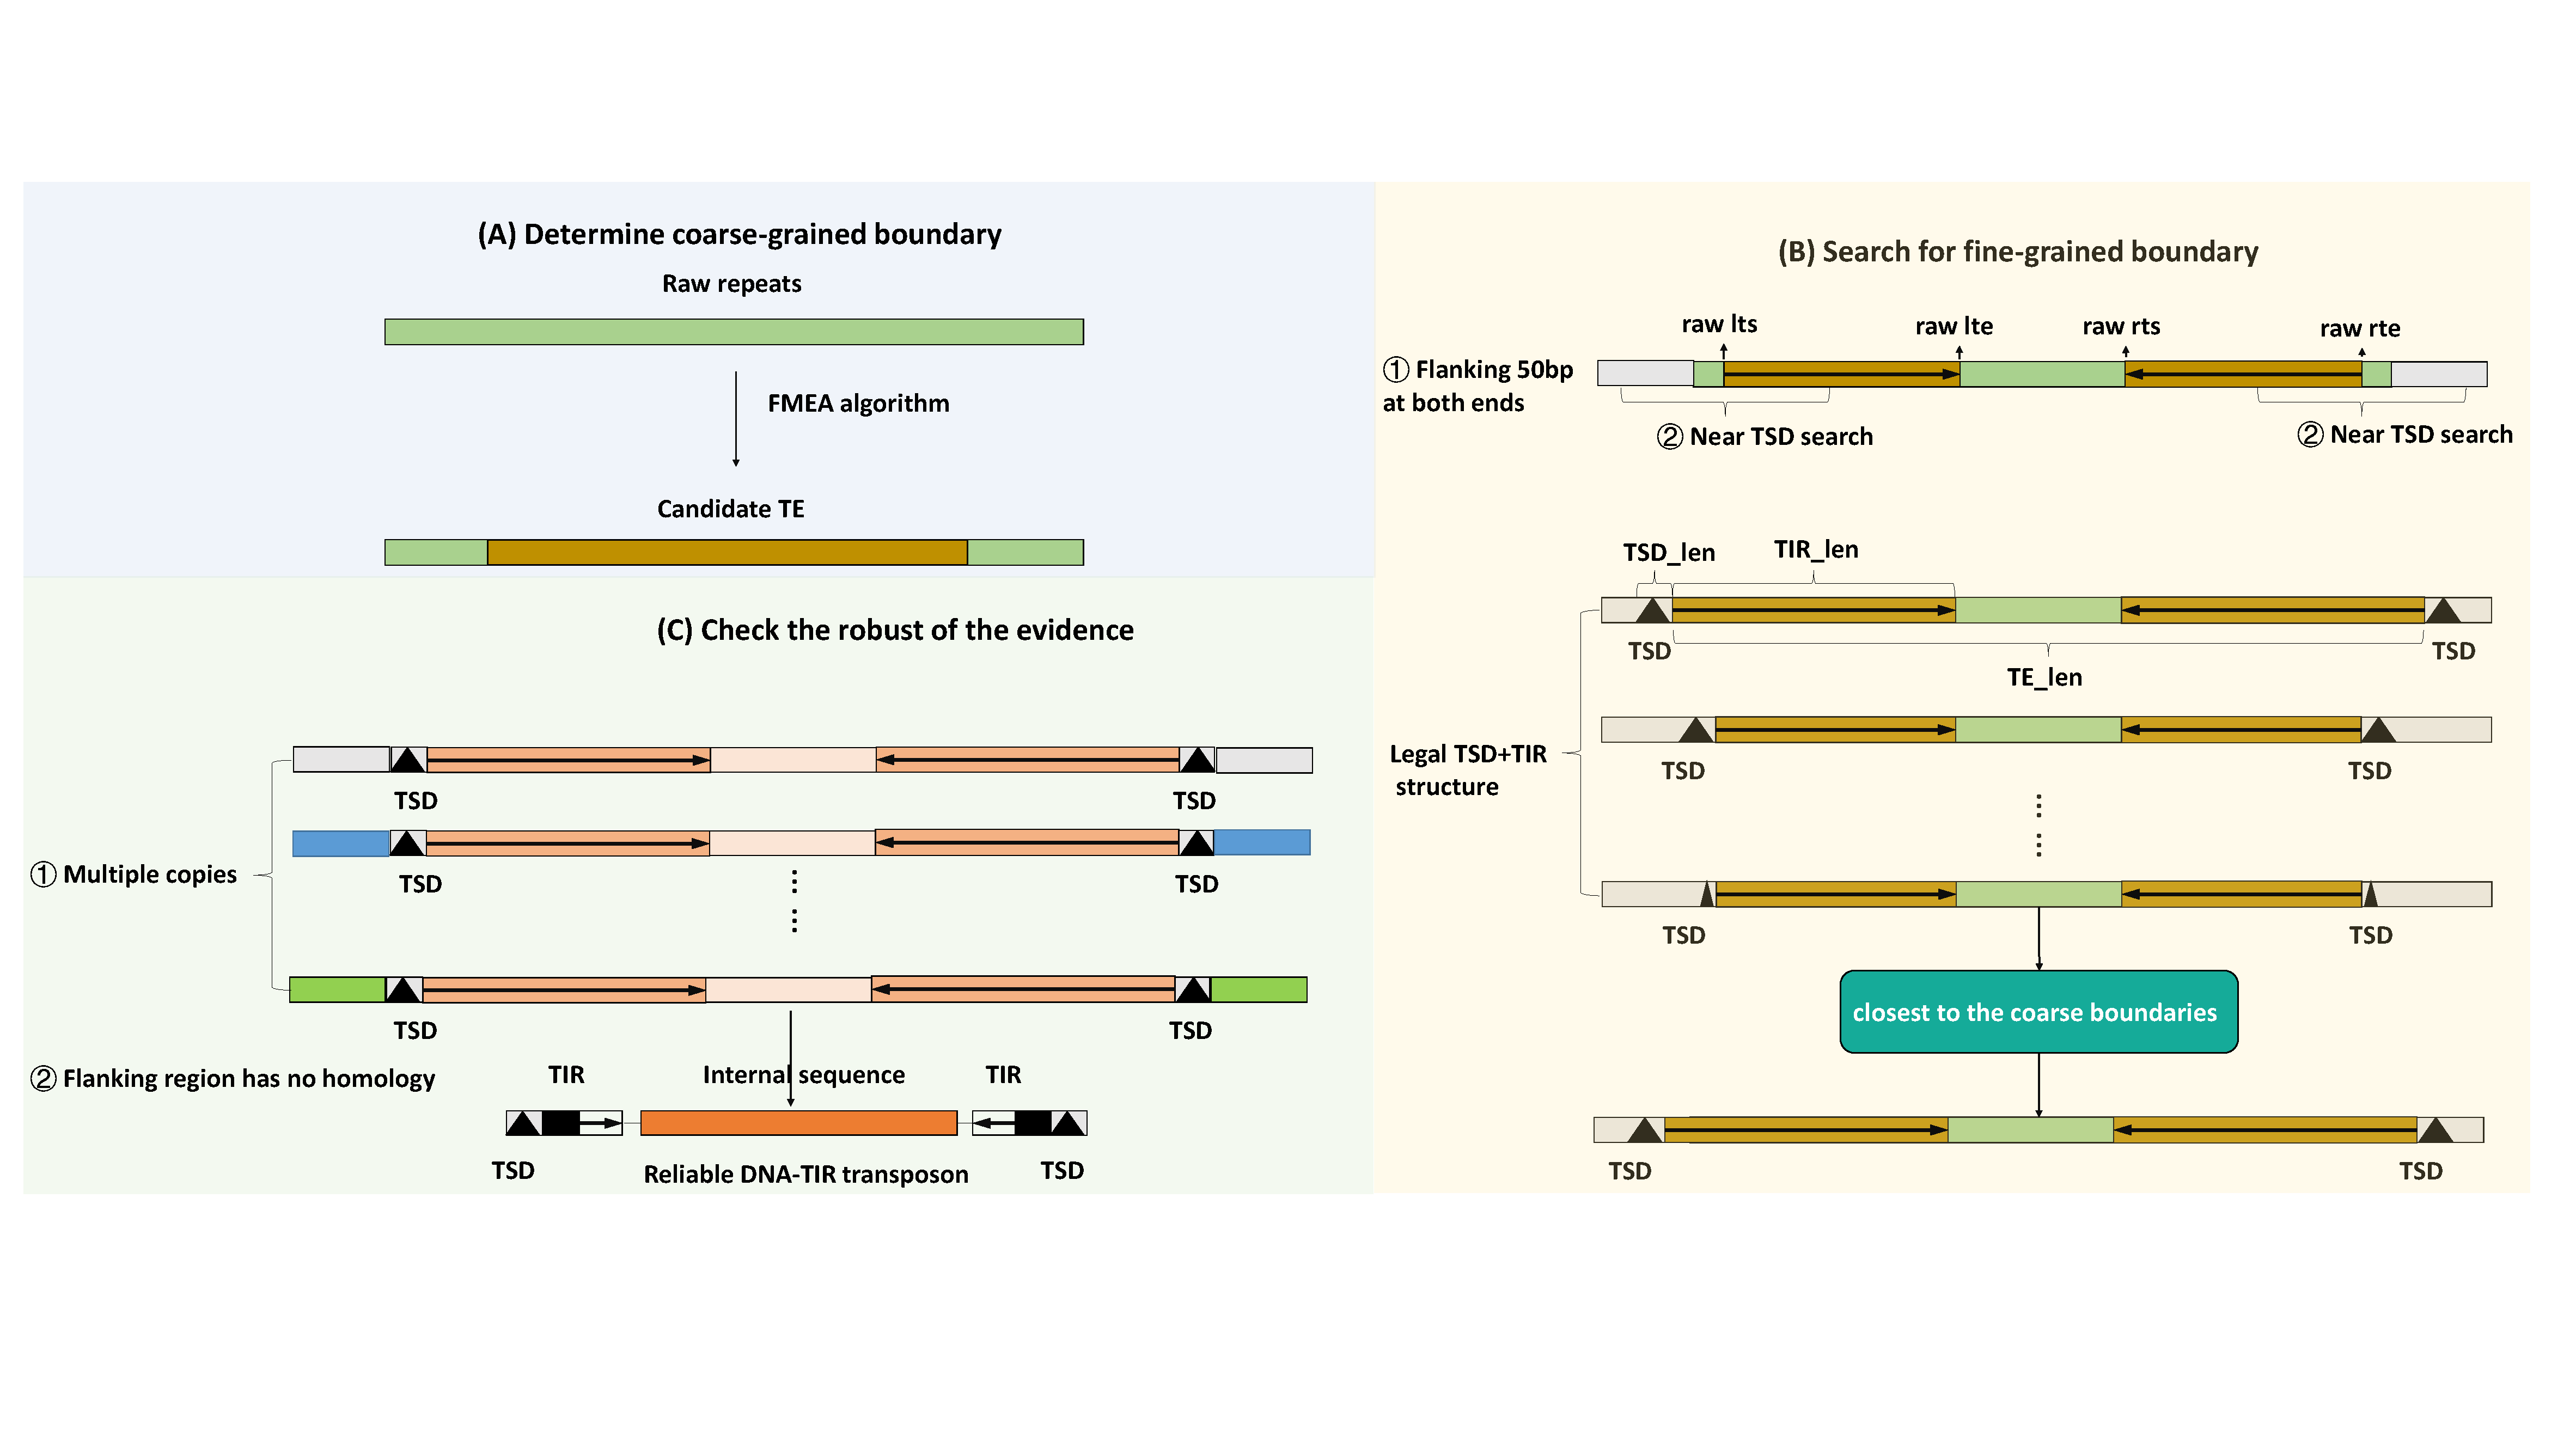
\includegraphics[width=1.0\textwidth]{figures/FineGrainedTE.pdf}}
%	\caption{Determine the fine-grained boundary of TIR. A the candidate TE sequences with coarse-grained boundaries are generated by the FMEA algorithm. B the candidate TIR elements with fine-grained boundaries are identified by exhaustively searching TSD; raw lts, lte, rts, and rte refer to the raw left/right terminal start/end positions, respectively. C the elements with multiple copies and non-homology flanking regions outside the boundaries are regarded as true transposons.}
%	\label{fig:fine_grained_TE}
%\end{figure}

\subsection*{Filtering false positive}
\subsubsection*{Sequencing gaps}
Gap sequences represent the most uncertainty in a genome assembly and are more likely to be associated with misassembly in a repetitive sequence\cite{ou2019benchmarking}. Candidate TE sequences that contain continuous gaps longer than 10 bp are excluded.

\subsubsection*{Tandem repeat}
Tandem Repeats Finder (TRF)\cite{benson1999tandem} is used to identify tandem repeats with parameters ``2 7 7 80 10 50 500 -f -d -m" (Additional file 2: Table S4). Sequences in which tandem repeats account for more than 50\% of the whole sequence are filtered out. At the same time, there are many false positives with tandem repeats at the terminal sequences of candidate LTRs and TIRs. Therefore, we take 100 bp and 20 bp of the terminal sequences in the candidate LTRs and TIRs, respectively. If there are more than 50\% tandem repeats in their terminal sequences, the candidate sequences are considered false positives and filtered out.

\subsubsection*{Fake TIR elements with LTR terminals}
We observed that some of the identified TIR candidates are actually LTR transposons (LTR terminals or LTR internals). The long LTR terminal may unexpectedly contain a short TIR terminal with legal TSDs and more than two full-length copies, which leads our TIR identification module to falsely identify it as a real TIR candidate. To filter out such false positives, the TIR candidates are aligned to the LTR sequences produced by the LTR module. The TIR candidates, which contain more than 80\% of an LTR element, are considered false positives and filtered out.

\subsubsection*{Filtering out false positives by homology outside the boundaries of copies}
False positives with TE structures are common in the genome, such as accidental terminal structures and TSD-like features. Our method of filtering false positives is based on the following principles, as shown in Fig. \ref{fig:framework}o: (i) A transposon, as a repetitive sequence, appears at least twice in the genome (regardless of the old TEs, whose instances have generated a lot of divergence after a long evolution), and (ii) the boundaries of transposons determine the starting and ending positions of repeats, and the region outside the boundaries should be regarded as random sequences and should not have homology.

Based on the above principles, we flank the copies of candidate TEs and then perform alignment between these flanked copies. If more than half of the copies have homology in the flanking region, the candidate sequence is regarded as a false positive and filtered out. These candidates are not real TEs, but rather long repeat sequences with TE-like structures. Since it is difficult for LTR-RTs to find their full-length copies, we have removed the limit of at least two occurrences of LTR identification.

\subsection*{Homology-Based TE Searching}
The autonomous LINE typically has a polyA tail and at least one RT and nuclease for transposition. The LINEs usually form TSDs at the insertion site, but their truncated 5$'$ ends make it hard to determine the true ends. SINEs have a similar structure to LINEs but are much shorter (80–500 bp), which are non-autonomous transposons that cannot transpose themselves and rely on other transposon enzymes to express, such as RT in LINEs.

Non-LTR elements (LINES and SINEs) are particularly challenging to discover due to their variability and undetectable structural signals. To date, no structure-based methods can identify LINEs, and fewer methods can produce SINEs predictions. Most methods, such as SINE-Finder\cite{wenke2011targeted} and SINE\_Scan\cite{mao2017sine_scan}, produce high rates of false positives and low sensitivity. 

To achieve high-precision non-LTR element annotation, we identify LINE and SINE transposons based on the method of homology search (Fig. \ref{fig:framework}j). Dfam is a public TE database, freely available under the Creative Commons Zero (``CC0") license. We extract known LINEs and SINEs from the Dfam library of RepeatMasker 4.1.2 to generate a non-LTR library. The non-LTR library is used to discover confident non-LTR elements by searching through the candidate TEs generated by the FMEA algorithm.

\subsection*{Generating the TE library}
\subsubsection*{Disjuncting nested TEs}
Nested TE, usually formed by transposons inserted into other transposons, has a complex chimeric structure. HiTE implements a method to disjunct the nested TEs by (i) removing the full-length TEs contained in other sequences with more than 95\% coverage and 95\% identity and connecting the remaining sequences; (ii) filtering out the sequence if the length is less than 100; otherwise, treating the remaining sequence as a new TE sequence; and (iii) iterating several times to disjunct heavily nested TEs.

\subsubsection*{Generating classified and consensus models}
HiTE generates TE consensus models using the clustering tool CD-HIT\cite{li2006cd} with the parameter ``-aS 0.95 -aL 0.95  -c 0.8 -G 0 -g 1 -A 80" (Additional file 2: Table S4). Notably, we divide the LTR-RTs into 5$'$ LTRs, 3$'$ LTRs, and LTR internal regions before clustering. To determine the classification information of TE, we use the RepeatClassifier module in RepeatModeler2\cite{flynn2020repeatmodeler2} to classify the TE consensus library.




%\subsection*{test}
%Text and results for this section, as per the individual journal's instructions for authors.
%
%In this section we examine the growth rate of the mean of $Z_0$, $Z_1$ and $Z_2$. In
%addition, we examine a common modeling assumption and note the
%importance of considering the tails of the extinction time $T_x$ in
%studies of escape dynamics.
%We will first consider the expected resistant population at $vT_x$ for
%some $v>0$, (and temporarily assume $\alpha=0$)
%%
%\[
%E \bigl[Z_1(vT_x) \bigr]=
%\int_0^{v\wedge
%1}Z_0(uT_x)
%\exp (\lambda_1)\,du .
%\]
%%
%If we assume that sensitive cells follow a deterministic decay
%$Z_0(t)=xe^{\lambda_0 t}$ and approximate their extinction time as
%$T_x\approx-\frac{1}{\lambda_0}\log x$, then we can heuristically
%estimate the expected value as
%%
%\begin{equation}\label{eqexpmuts}
%\begin{aligned}[b]
%&      E\bigl[Z_1(vT_x)\bigr]\\
%&\quad      = \frac{\mu}{r}\log x
%\int_0^{v\wedge1}x^{1-u}x^{({\lambda_1}/{r})(v-u)}\,du .
%\end{aligned}
%\end{equation}
%%


\section*{Supplementary information}

%%%%%%%%%%%%%%%%%%%%%%%%%%%%%%%%%%%%%%%%%%%%%%
%%                                          %%
%% Backmatter begins here                   %%
%%                                          %%
%%%%%%%%%%%%%%%%%%%%%%%%%%%%%%%%%%%%%%%%%%%%%%

\begin{backmatter}

\section*{Acknowledgements}%% if any
This work was carried out in part using computing resources at the High Performance Computing Center of Central South University.

\section*{Funding}%% if any
This work has been supported by the National Natural Science Foundation of China under Grant: No.61772557 and No.62002388, Hunan Provincial Science and technology Program (No.2018wk4001), 111 Project (No.B18059), Fundamental Research Funds for the Central Universities of Central South University (2021zzts0208).

%\section*{Abbreviations}%% if any
%Text for this section\ldots

\section*{Availability of data and materials}%% if any
All data, code, and scripts are freely available at https://github.com/CSU-KangHu/HiTE.

\section*{Ethics approval and consent to participate}%% if any
Not applicable.

\section*{Competing interests}
The authors declare that they have no competing interests.

\section*{Consent for publication}%% if any
Not applicable.

\section*{Authors' contributions}
KH and JW conceived the study. JW supervised the project. KH conducted the analyses. KH developed the HiTE package. KH and JW wrote the manuscript. All authors read and approved the final manuscript.

%\section*{Authors' information}%% if any
%Text for this section\ldots

%%%%%%%%%%%%%%%%%%%%%%%%%%%%%%%%%%%%%%%%%%%%%%%%%%%%%%%%%%%%%
%%                  The Bibliography                       %%
%%                                                         %%
%%  Bmc_mathpys.bst  will be used to                       %%
%%  create a .BBL file for submission.                     %%
%%  After submission of the .TEX file,                     %%
%%  you will be prompted to submit your .BBL file.         %%
%%                                                         %%
%%                                                         %%
%%  Note that the displayed Bibliography will not          %%
%%  necessarily be rendered by Latex exactly as specified  %%
%%  in the online Instructions for Authors.                %%
%%                                                         %%
%%%%%%%%%%%%%%%%%%%%%%%%%%%%%%%%%%%%%%%%%%%%%%%%%%%%%%%%%%%%%

% if your bibliography is in bibtex format, use those commands:
\bibliographystyle{bmc-mathphys} % Style BST file (bmc-mathphys, vancouver, spbasic).
\bibliography{bmc_article}      % Bibliography file (usually '*.bib' )
% for author-year bibliography (bmc-mathphys or spbasic)
% a) write to bib file (bmc-mathphys only)
% @settings{label, options="nameyear"}
% b) uncomment next line
%\nocite{label}

% or include bibliography directly:
% \begin{thebibliography}
% \bibitem{b1}
% \end{thebibliography}

%%%%%%%%%%%%%%%%%%%%%%%%%%%%%%%%%%%
%%                               %%
%% Figures                       %%
%%                               %%
%% NB: this is for captions and  %%
%% Titles. All graphics must be  %%
%% submitted separately and NOT  %%
%% included in the Tex document  %%
%%                               %%
%%%%%%%%%%%%%%%%%%%%%%%%%%%%%%%%%%%

%%
%% Do not use \listoffigures as most will included as separate files

\section*{Figures}
%\begin{figure}[h!]
%  \caption{Sample figure title}
%\end{figure}

%\begin{figure}[h!]
%	%\centerline{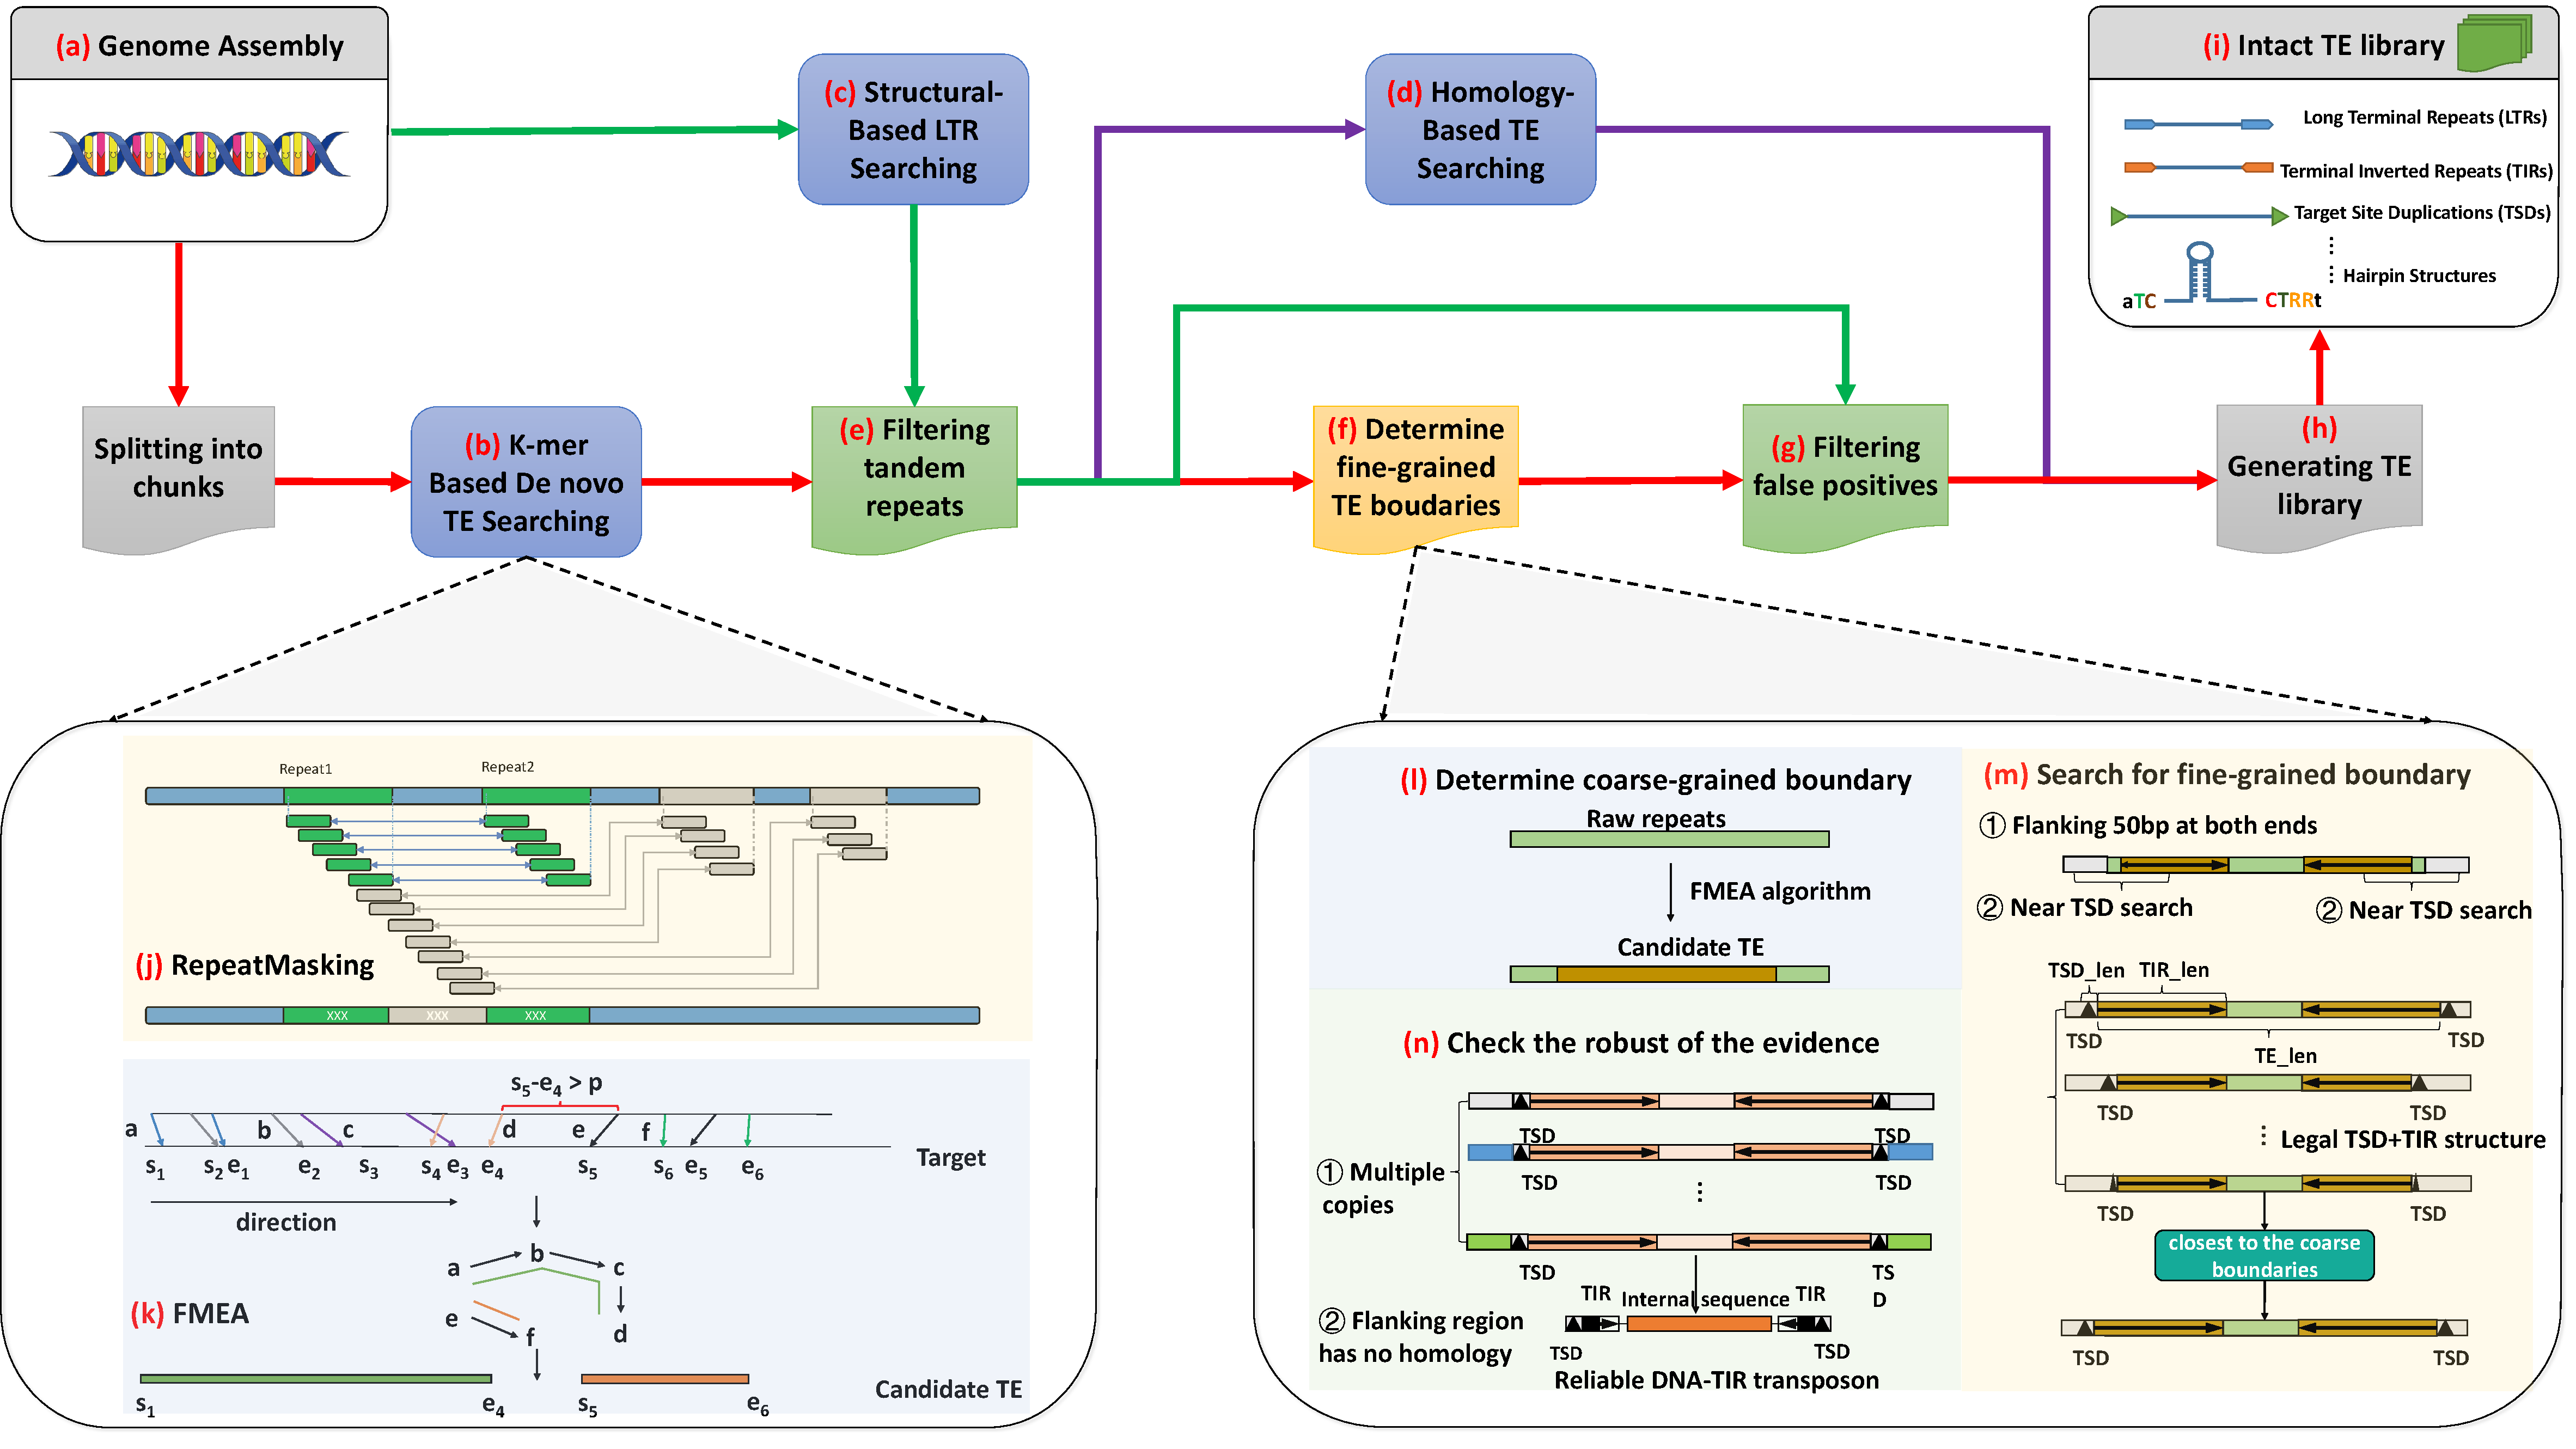
\includegraphics[width=1.0\textwidth]{figures/Framework1.pdf}}
%	\caption{The workflow of HiTE. \textbf{a} HiTE takes the genome assembly as input; \textbf{b} the genome assembly is split into chunks to reduce the amount of single-round computation; \textbf{c, i, and j} three main modules of HiTE are used to identify different types of TEs; \textbf{d} the candidates with a large amount of tandem repeats are regarded as false positives and are filtered out; \textbf{e} the fine-grained boundaries of TEs are determined using signature-based methods; \textbf{f} the candidates with repetitive flanking sequences within copies that are parts of a larger repetitive element are considered false positives and are filtered out; \textbf{g} CD-HIT and RepeatClassifier are used to generate TE libraries; \textbf{h} the TE libraries generated by HiTE contain intact TE structures; \textbf{k} the candidate repeat regions within the genome are masked based on the low-frequency \emph{k}-mer masking method, RepeatMasking; \textbf{l} the coarse boundaries of TEs are identified based on the fault-tolerant mapping expansion algorithm, FMEA; and \textbf{m, n, and o} the true ends of TEs are discovered by searching for the fine-grained TE boundaries, and the robust evidence of true TEs are checked by non-homology flanking regions within multiple copies.}
%	\label{fig:framework}
%\end{figure}
%
%\begin{figure}[h!]
%	%\centerline{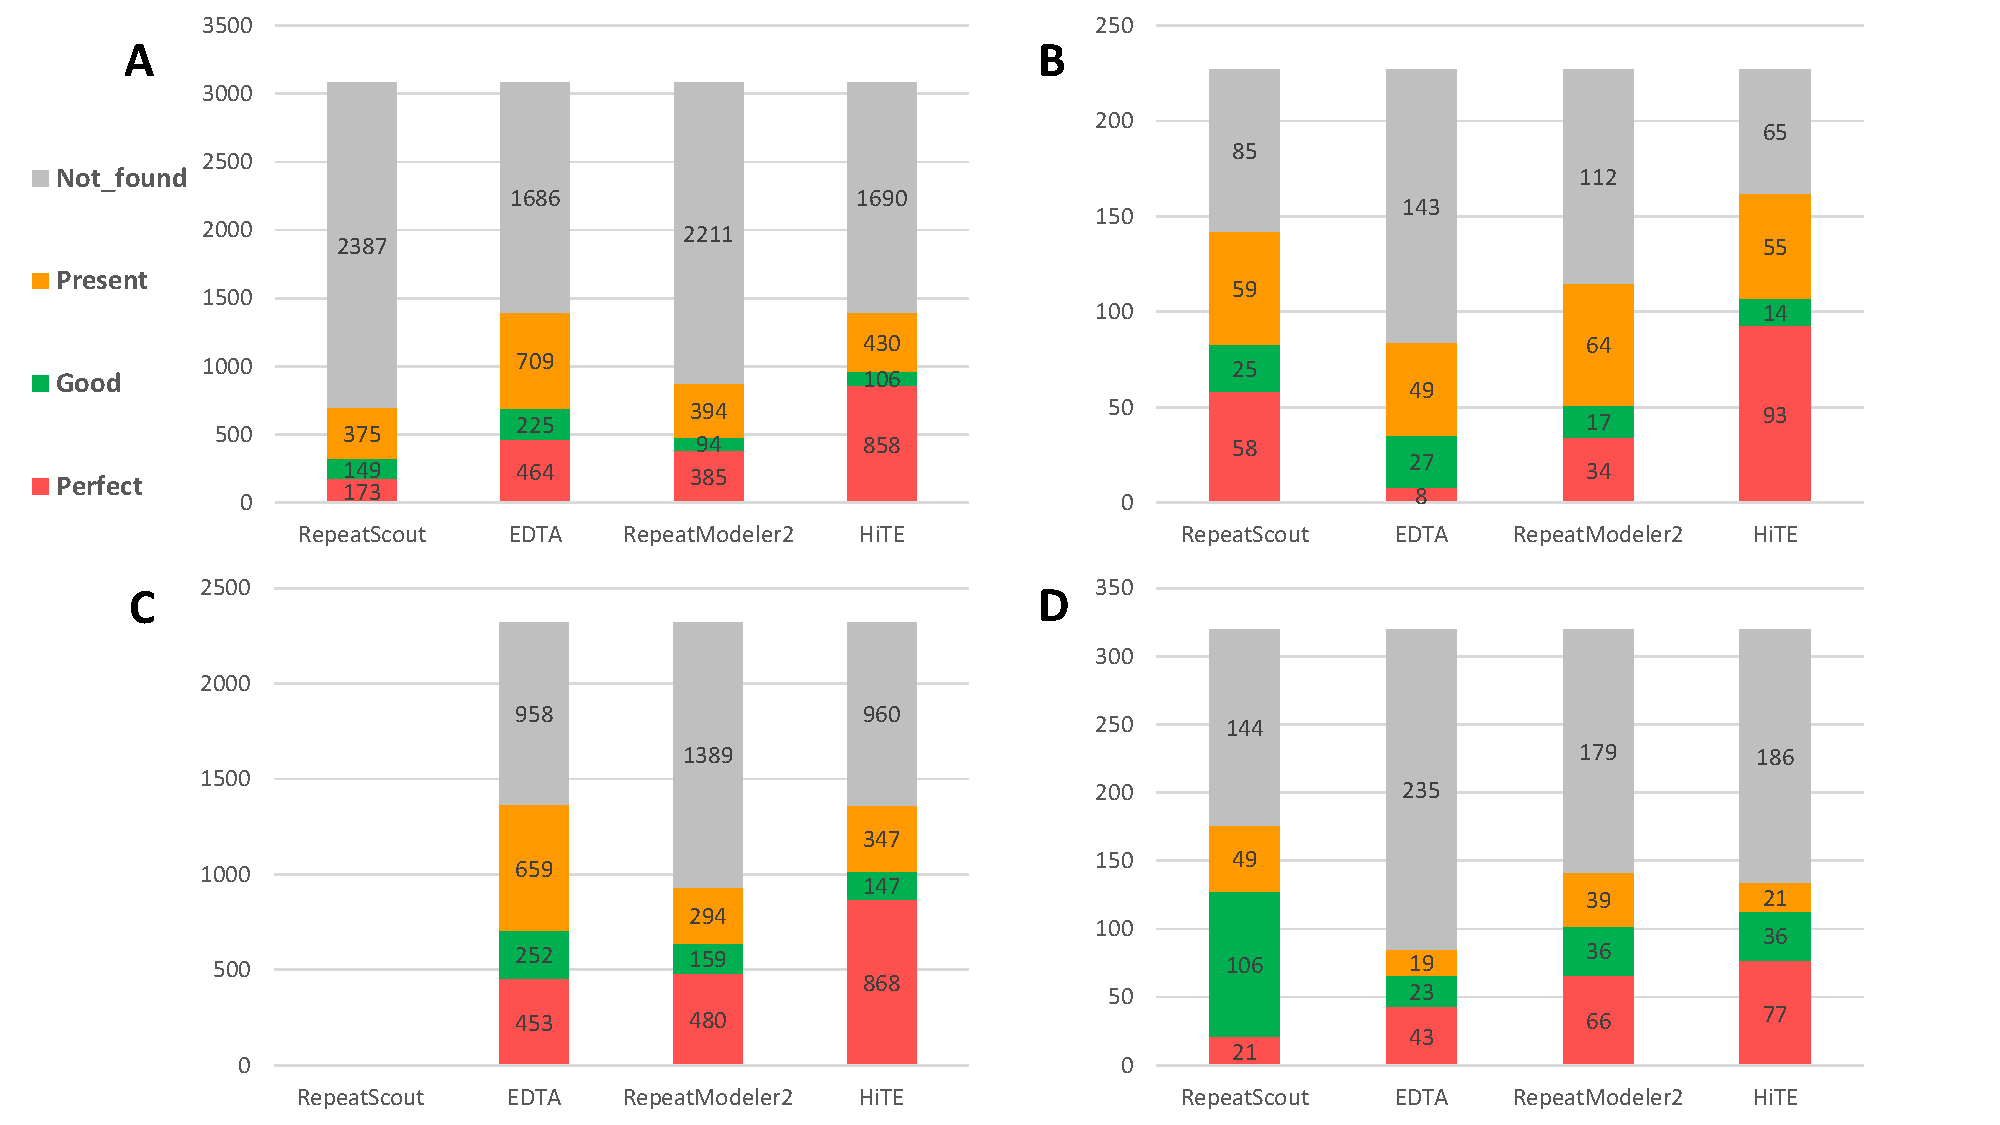
\includegraphics[width=1.0\textwidth]{figures/RM2Results.pdf}}
%	\caption{Performance of general-purpose TE annotators based on benckmarking method of RepeatModeler2. \textbf{a} Performance using benckmarking method of RepeatModeler2 based on O. sativa genome. \textbf{b} Performance using benckmarking method of RepeatModeler2 based on C. briggsae genome. \textbf{c} Performance using benckmarking method of RepeatModeler2 based on D. rerio genome. \textbf{d} Performance using benckmarking method of RepeatModeler2 based on D. melanogaster genome.}
%	\label{fig:rm2_results}
%\end{figure}
%
%\begin{figure}[h!]
%	%\centerline{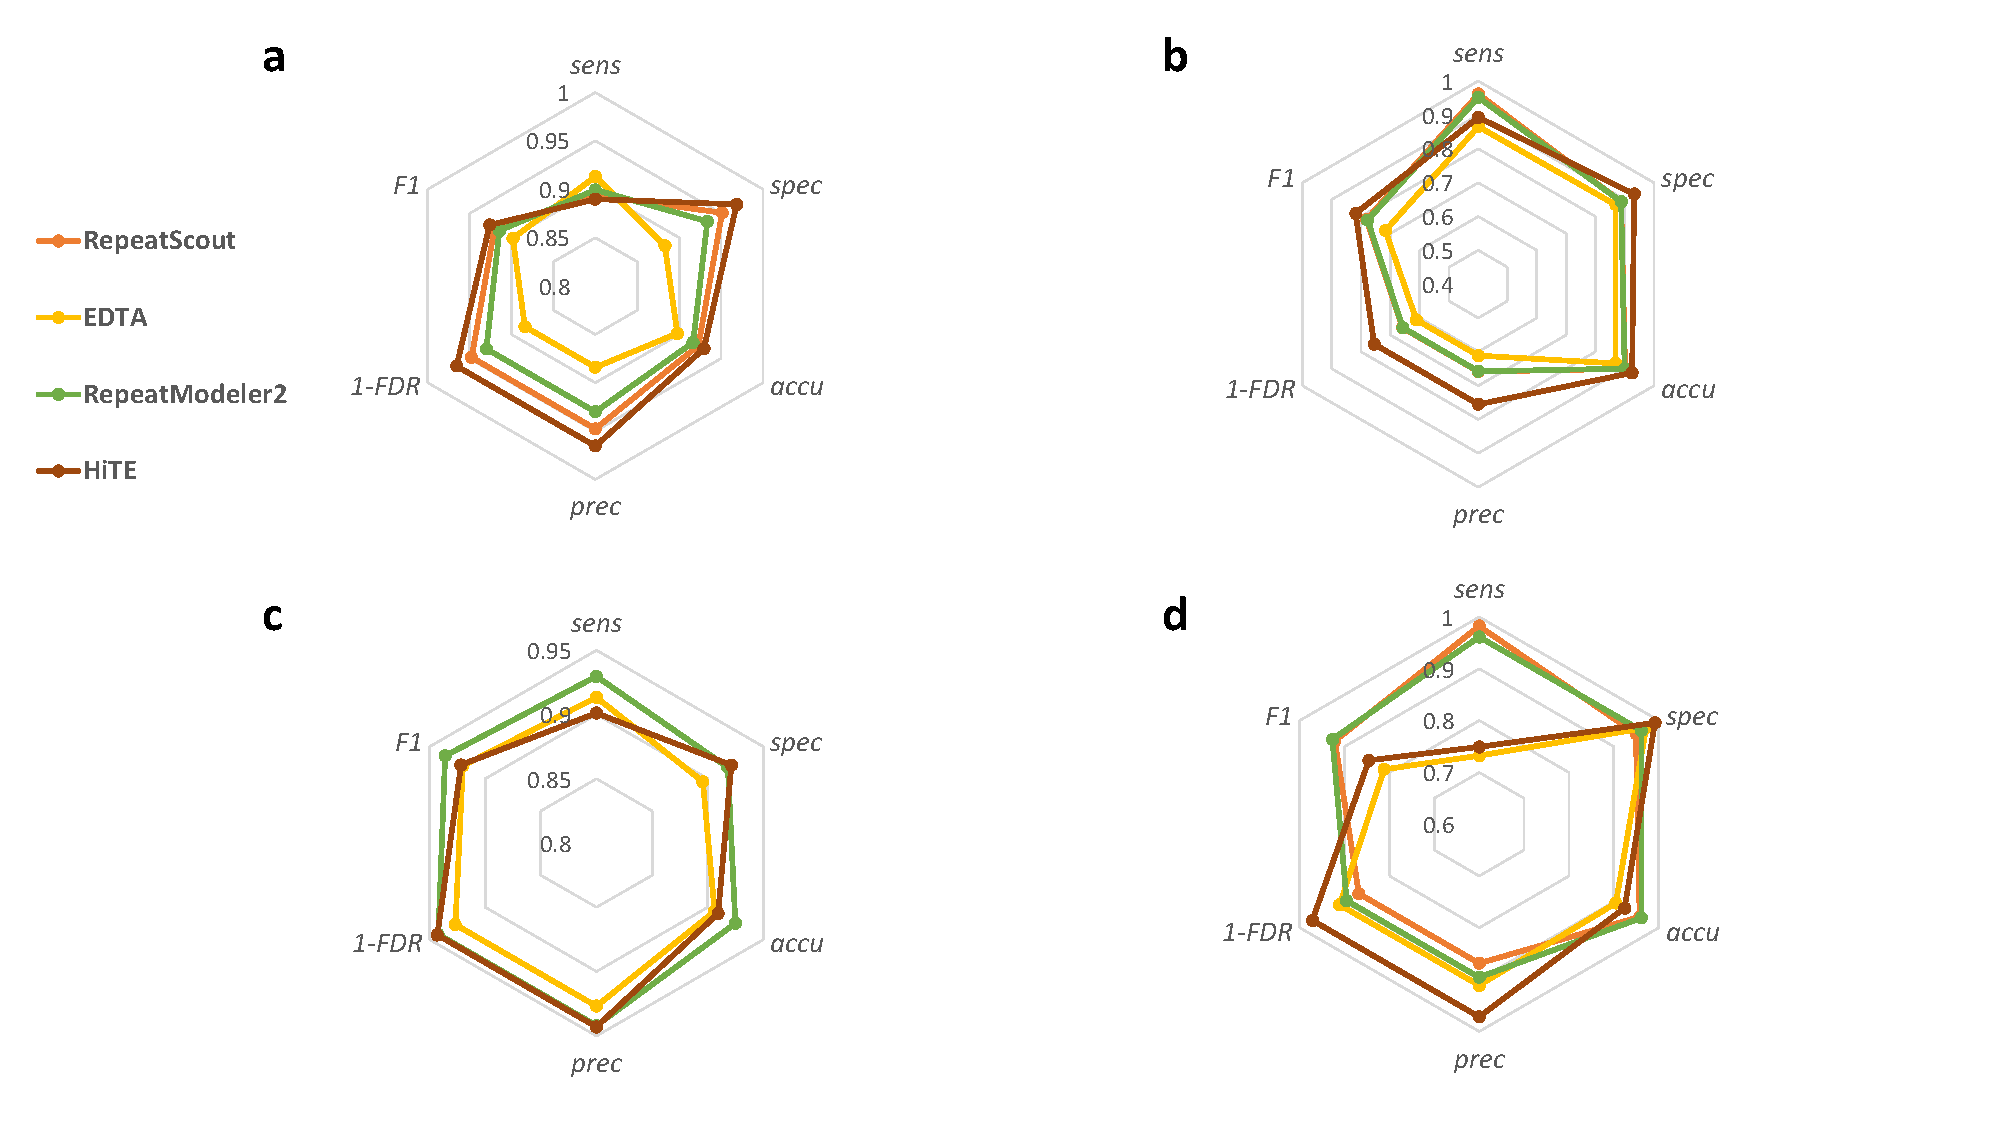
\includegraphics[width=1.0\textwidth]{figures/EDTAResults.pdf}}
%	\caption{Performance of general-purpose TE annotators based on benckmarking method of EDTA.  \textbf{a} Performance using benckmarking method of EDTA based on O. sativa genome. \textbf{b} Performance using benckmarking method of EDTA based on C. briggsae genome. \textbf{c} Performance using benckmarking method of EDTA based on D. rerio genome. \textbf{d} Performance using benckmarking method of EDTA based on D. melanogaster genome.}
%	\label{fig:edta_results}
%\end{figure}
%
%\begin{figure}[h!]
%	%\centerline{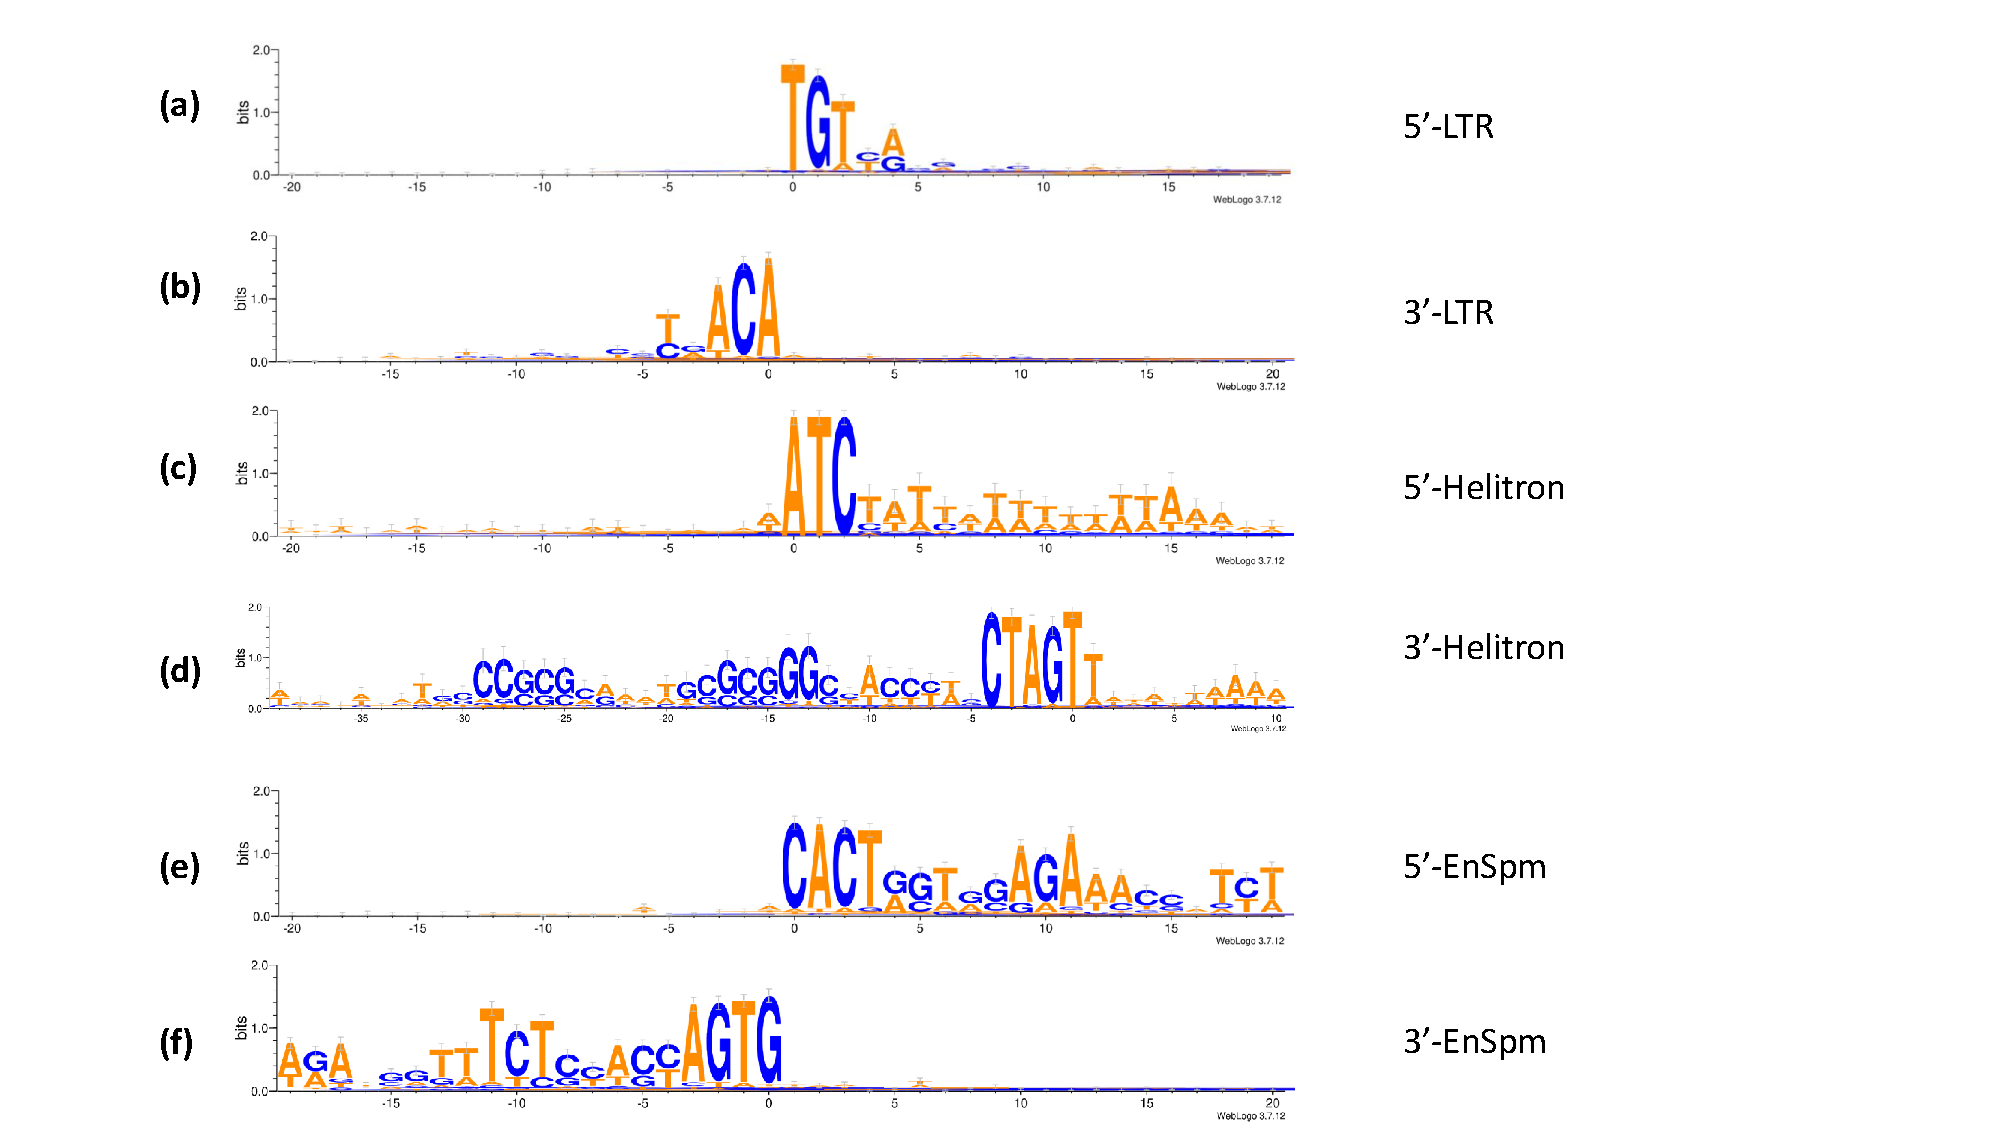
\includegraphics[width=1.0\textwidth]{figures/SeqLogos.pdf}}
%	\caption{Sequence logos of terminal and flanking sequences of LTR, Helitron, and EnSpm candidates generated by HiTE. \textbf{(a)} 5$'$ terminal of LTR candidates with the starting position labeled as 0; \textbf{(b)} 3$'$ terminal of LTR candidates with the last position labeled as 0; \textbf{(c)} 5$'$ terminal of Helitron candidates with the starting position labeled as 1; \textbf{(d)} 3$'$ terminal of Helitron candidates with the last position labeled as -1; \textbf{(e)} 5$'$ terminal of EnSpm candidates with the starting position labeled as 0; \textbf{(f)} 3$'$ terminal of EnSpm candidates with the last position labeled as 0.}
%	\label{fig:seq_logos}
%\end{figure}
%
%\begin{figure}[h!]
%	%\centerline{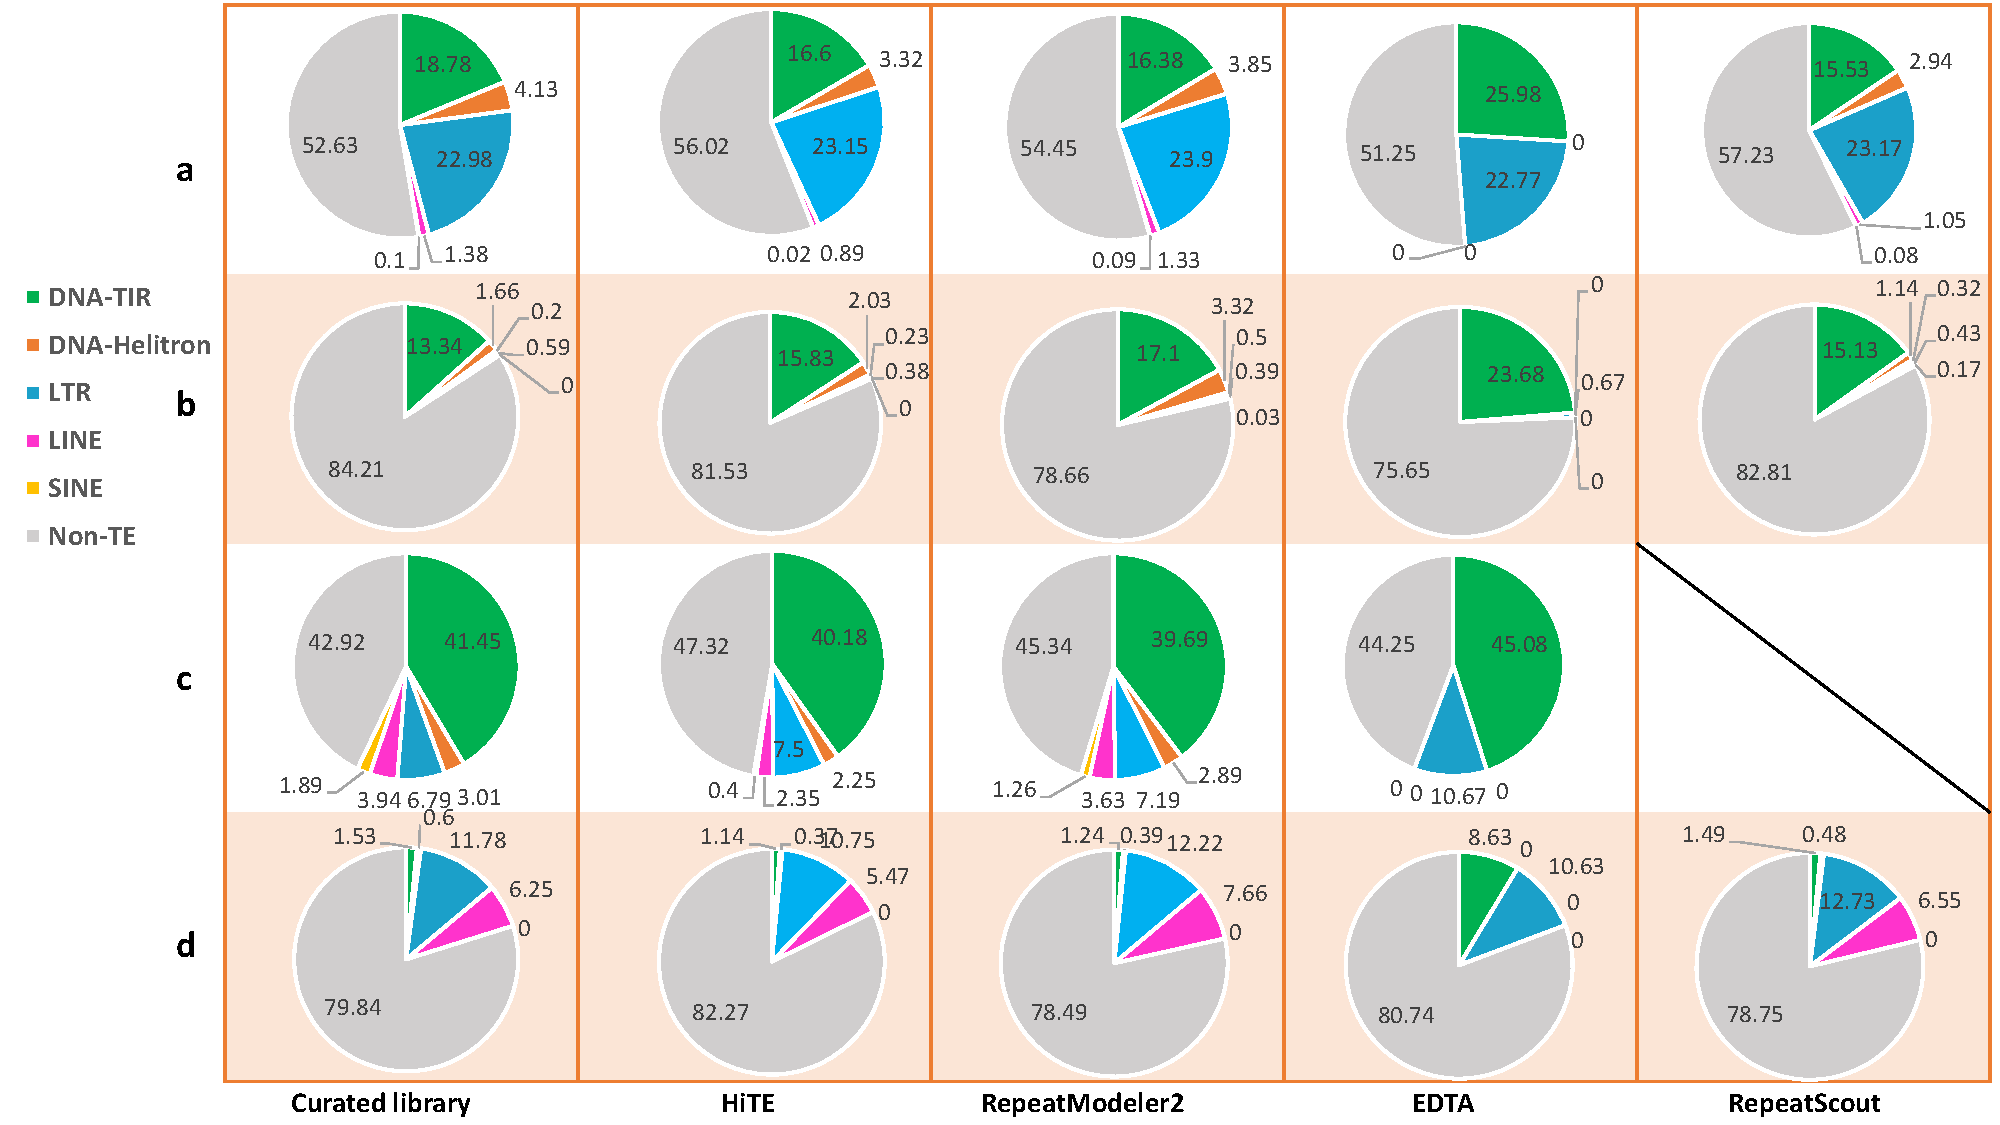
\includegraphics[width=1.0\textwidth]{figures/RatioResults.pdf}}
%	\caption{Percent of genome masked by each major subclass based on five types of TE libraries, generated by manually curated, HiTE, RepeatModeler2, EDTA, and RepeatScout, respectively. \textbf{a} The percentage of the O. sativa genome masked by TE libraries. \textbf{b} The percentage of the C. briggsae genome masked by TE libraries. \textbf{c} The percentage of the D. rerio genome masked by TE libraries. \textbf{d} The percentage of the D. melanogaster genome masked by TE libraries. }
%	\label{fig:ratio_results}
%\end{figure}
%
%\begin{figure}[h!]
%	%\centerline{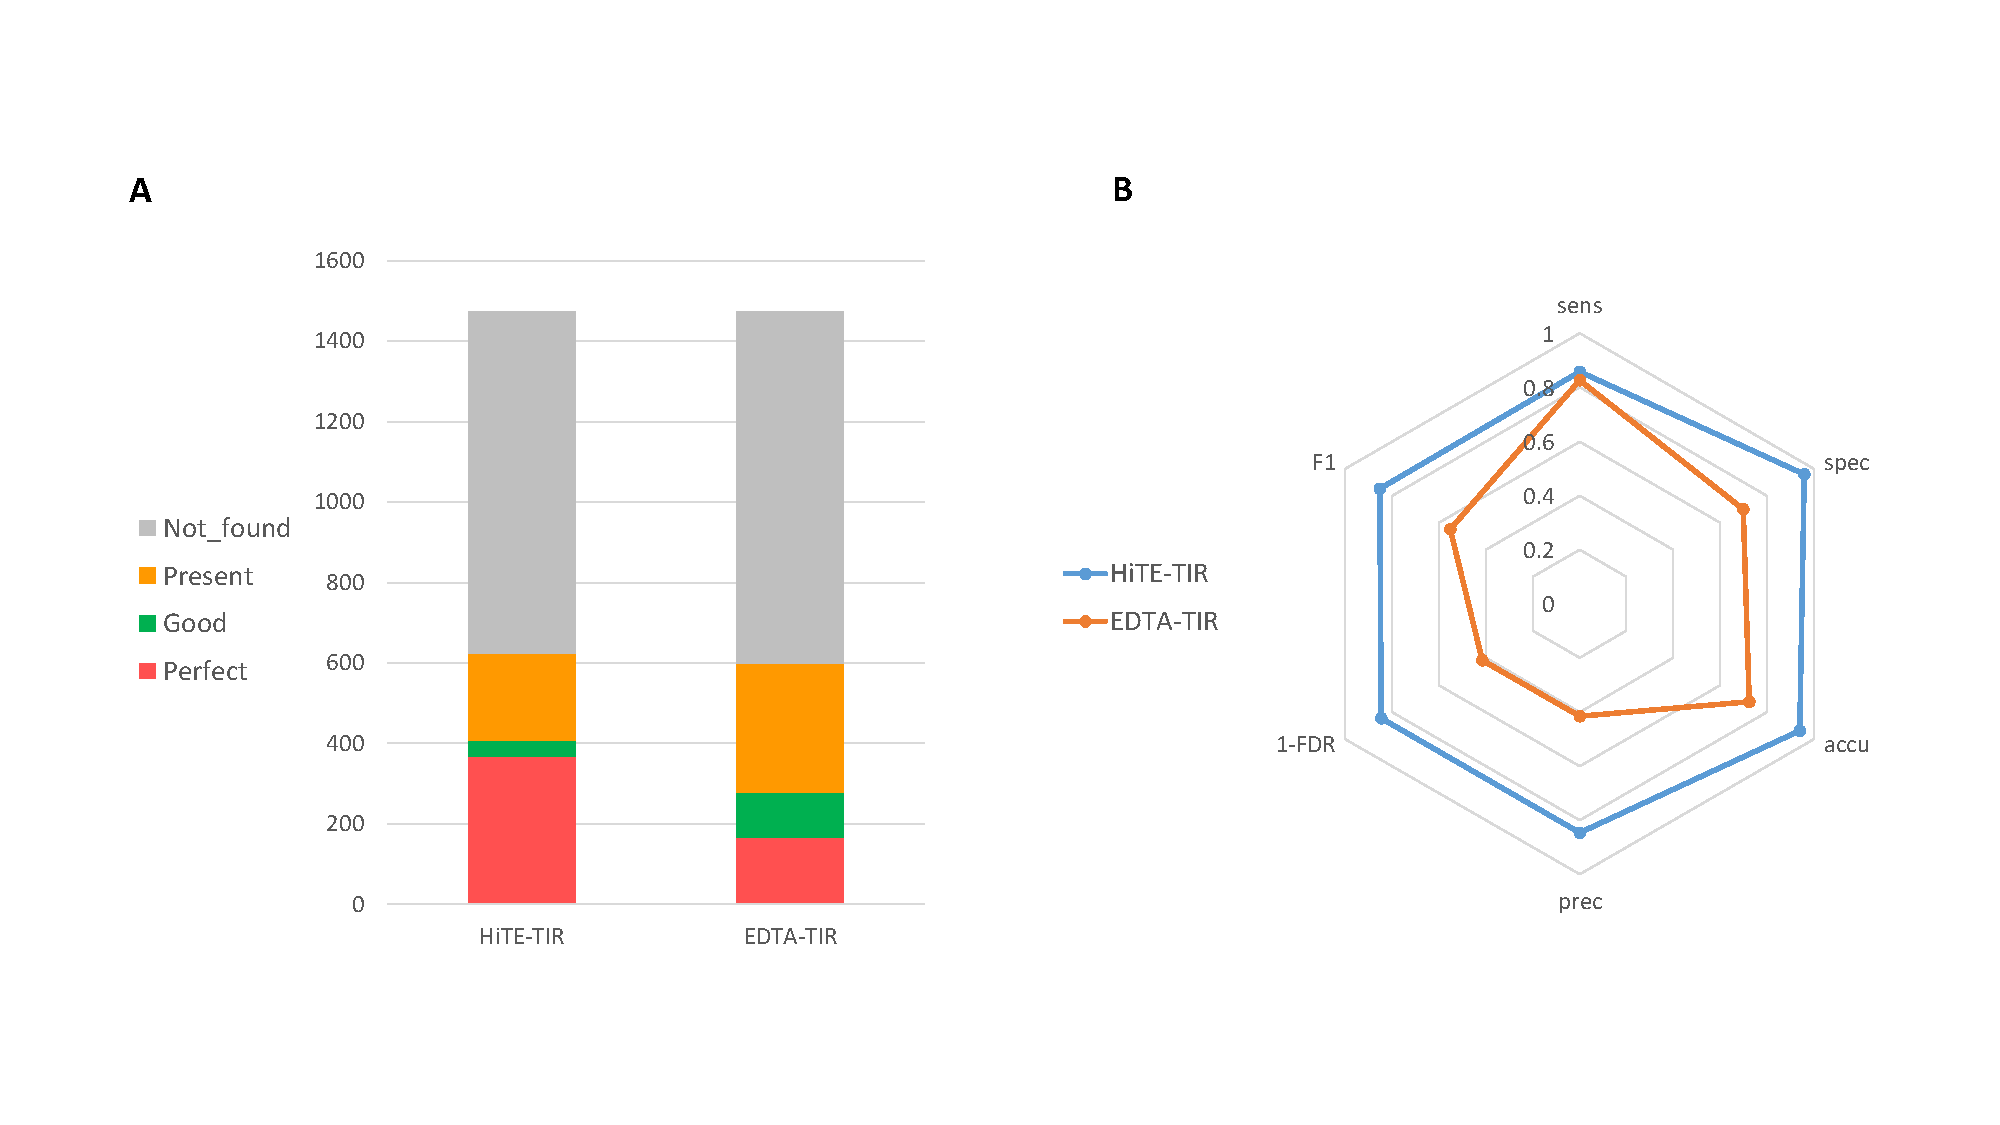
\includegraphics[width=1.0\textwidth]{figures/TIRResults.pdf}}
%	\caption{Performance of TIR annotators. \textbf{a} the performance based on benckmarking method of RepeatModeler2 and \textbf{b} the performance based on benckmarking method of EDTA.}
%	\label{fig:tir_results}
%\end{figure}
%
%\begin{figure}[h!]
%	%\centerline{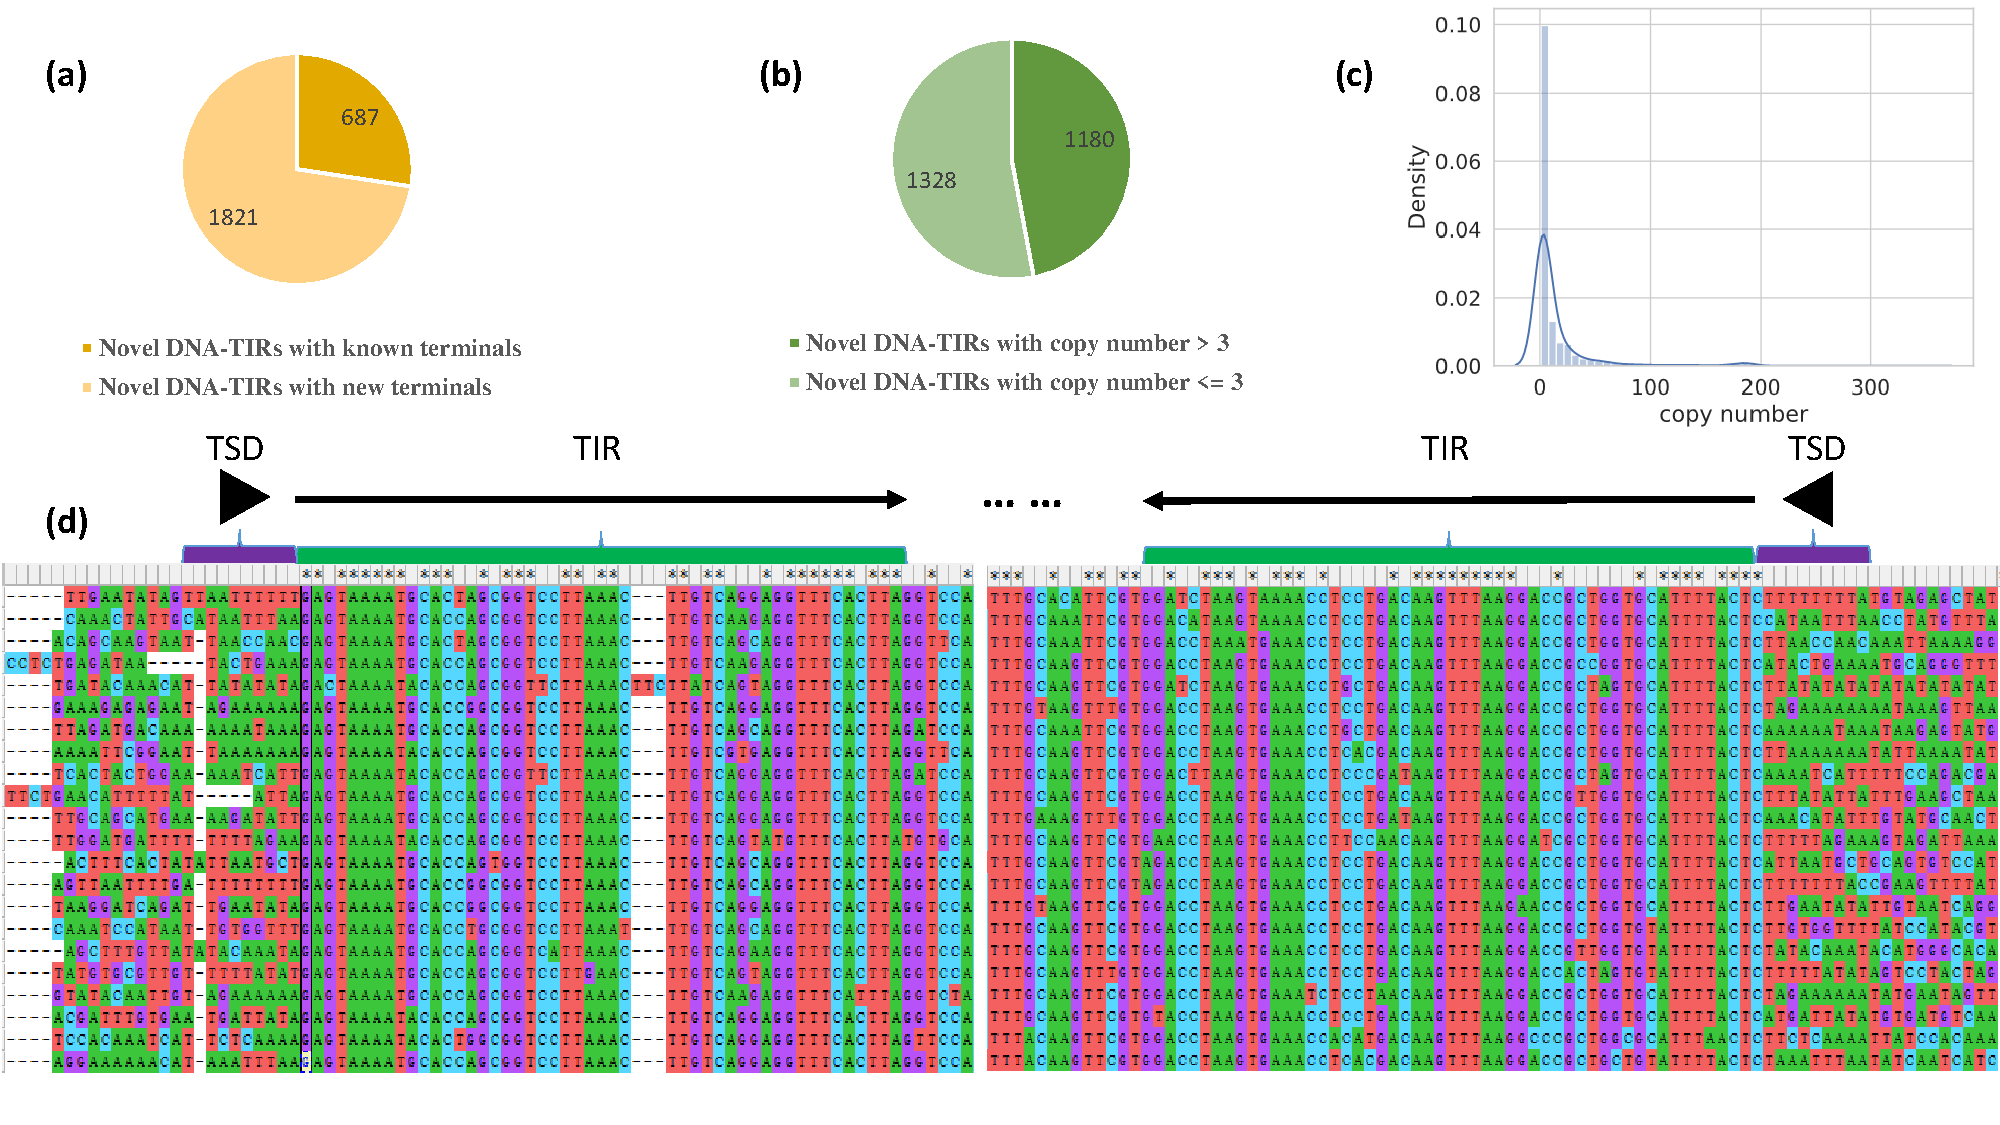
\includegraphics[width=1.0\textwidth]{figures/NovelTIRs.pdf}}
%	\caption{Characteristic of novel TIR elements identified by HiTE. \textbf{a} the number of novel TIR elements with different types of terminals; \textbf{b} the number of novel TIR elements with copy numbers $>$ 3 and $<=$ 3; \textbf{c} the distribution of copy numbers of TIR elements identified by HiTE; and \textbf{d} the multiple sequence alignment example of a novel TIR element discovered by HiTE.}
%	\label{fig:novel_tirs}
%\end{figure}
%
%\begin{figure}[h!]
%	%\centerline{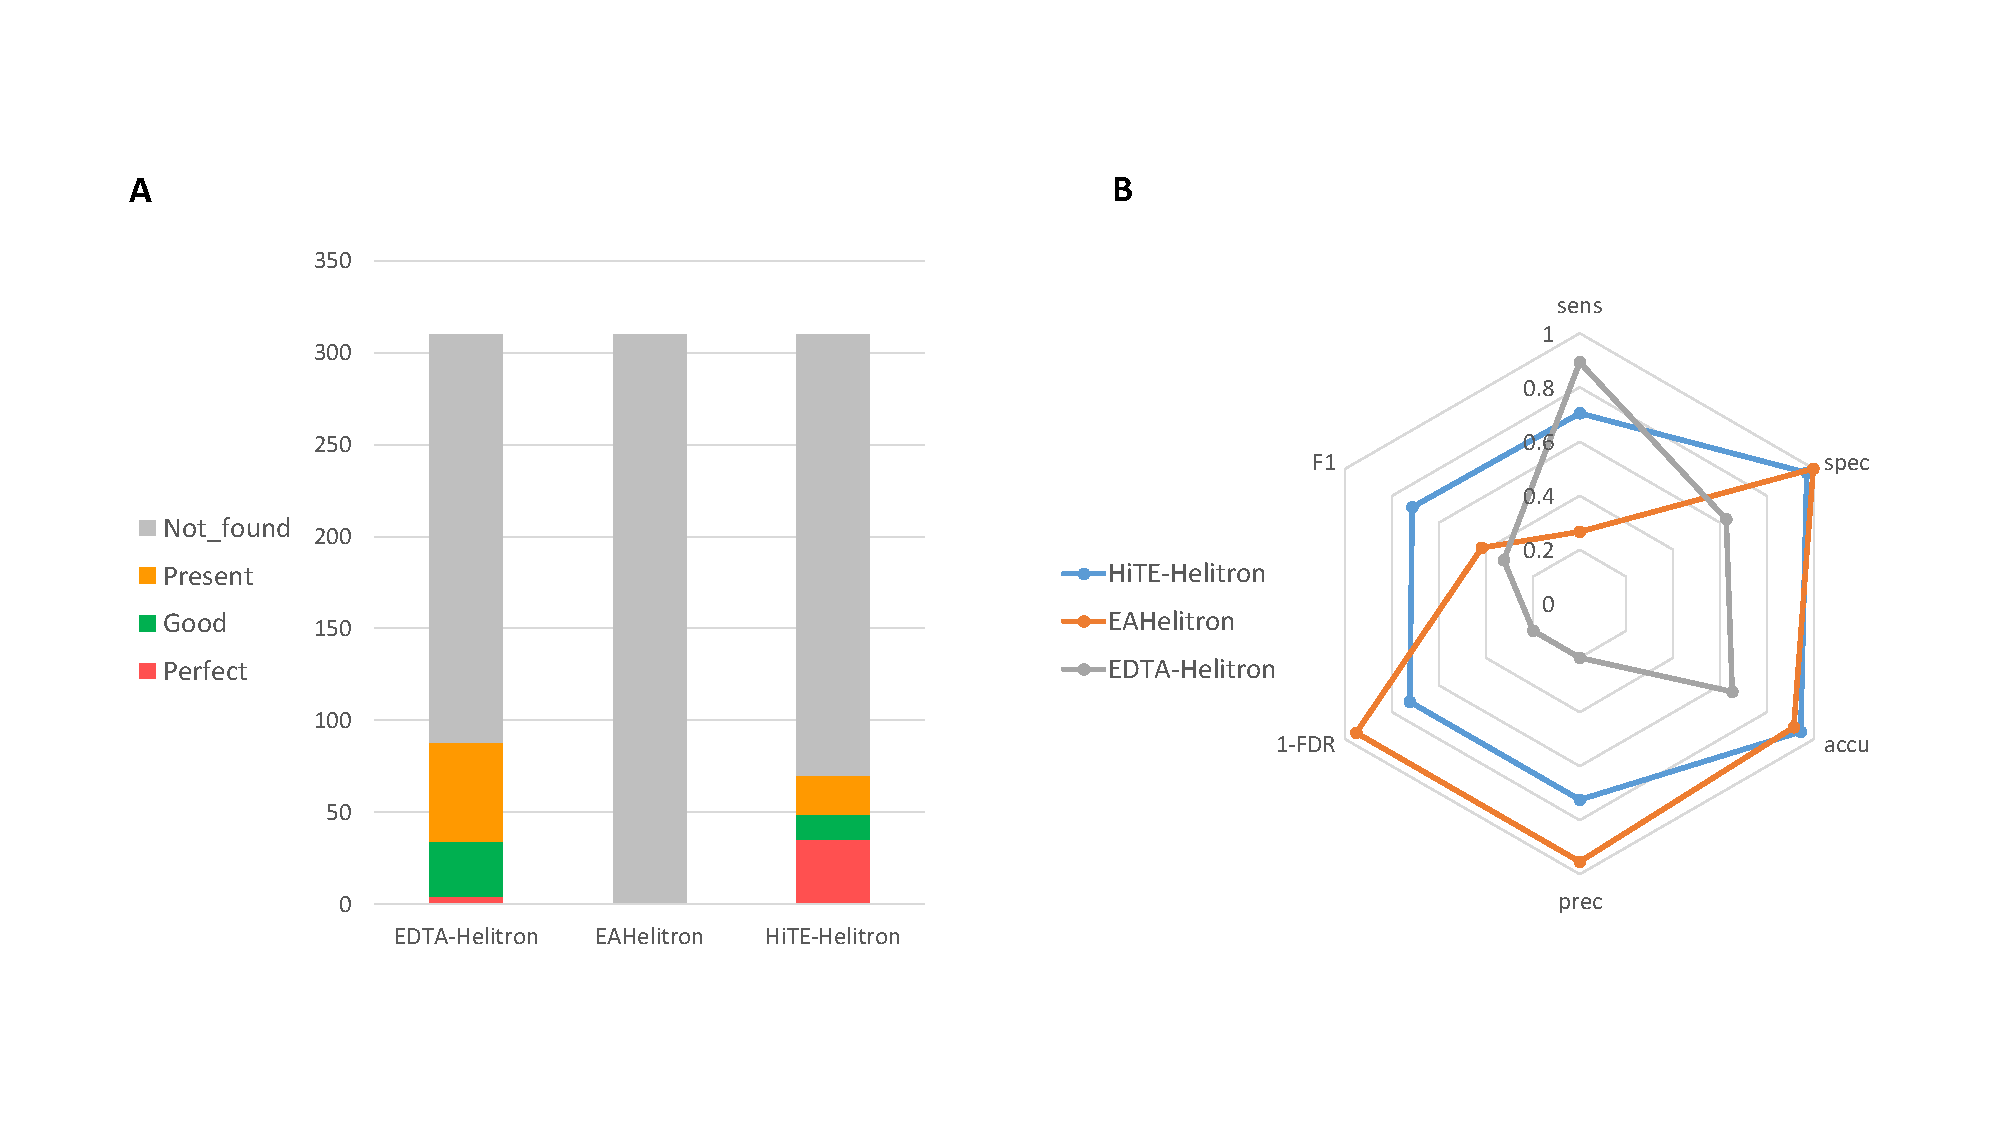
\includegraphics[width=1.0\textwidth]{figures/HelitronResults.pdf}}
%	\caption{Performance of Helitron annotators. \textbf{a} the performance based on benckmarking method of RepeatModeler2 and \textbf{b} the performance based on benckmarking method of EDTA.}
%	\label{fig:helitron_results}
%\end{figure}
%
%\begin{figure}[h!]
%	%\centerline{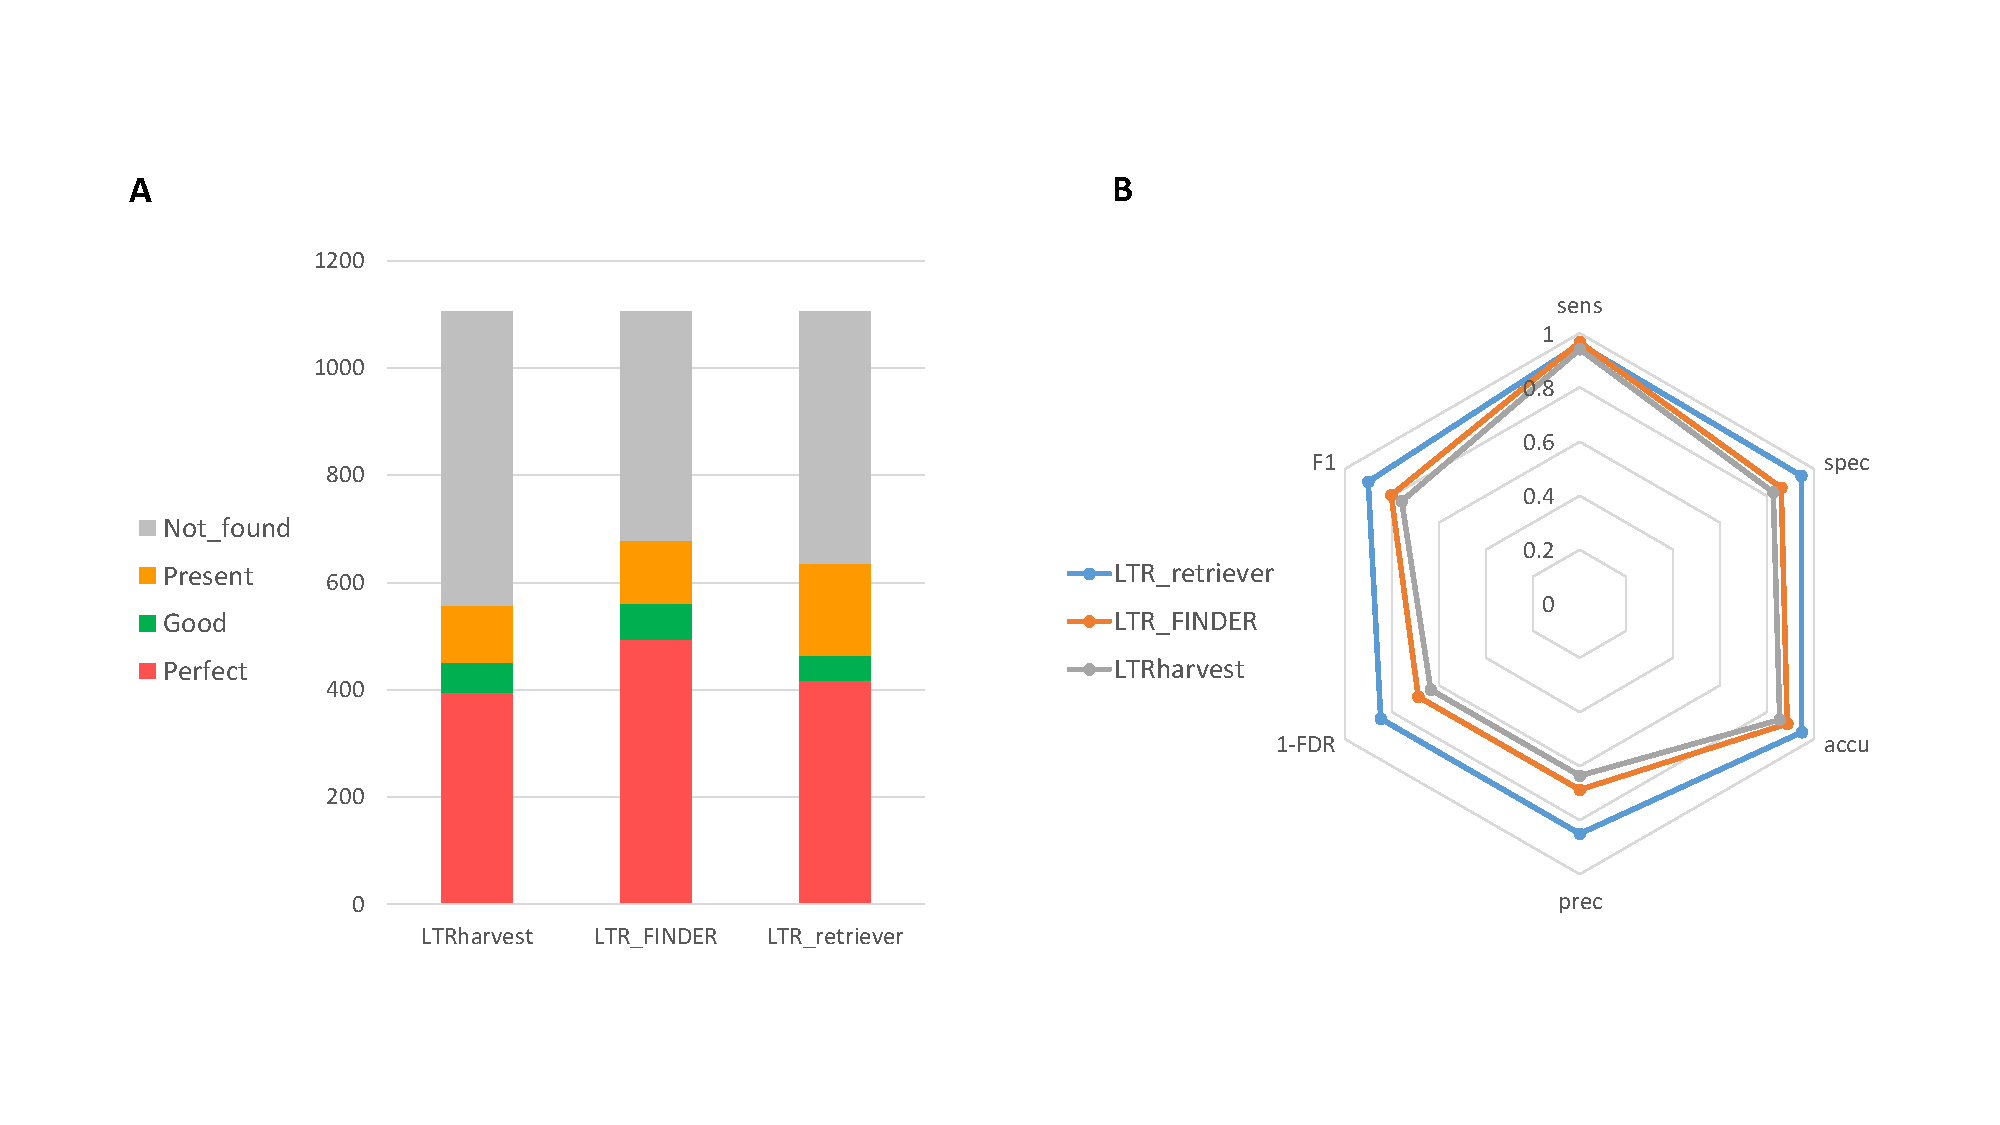
\includegraphics[width=1.0\textwidth]{figures/LTRResults.pdf}}
%	\caption{Performance of LTR annotators. \textbf{a} the performance based on benckmarking method of RepeatModeler2 and \textbf{b} the performance based on benckmarking method of EDTA.}
%	\label{fig:ltr_results}
%\end{figure}
%
%\begin{figure}[h!]
%	%\centerline{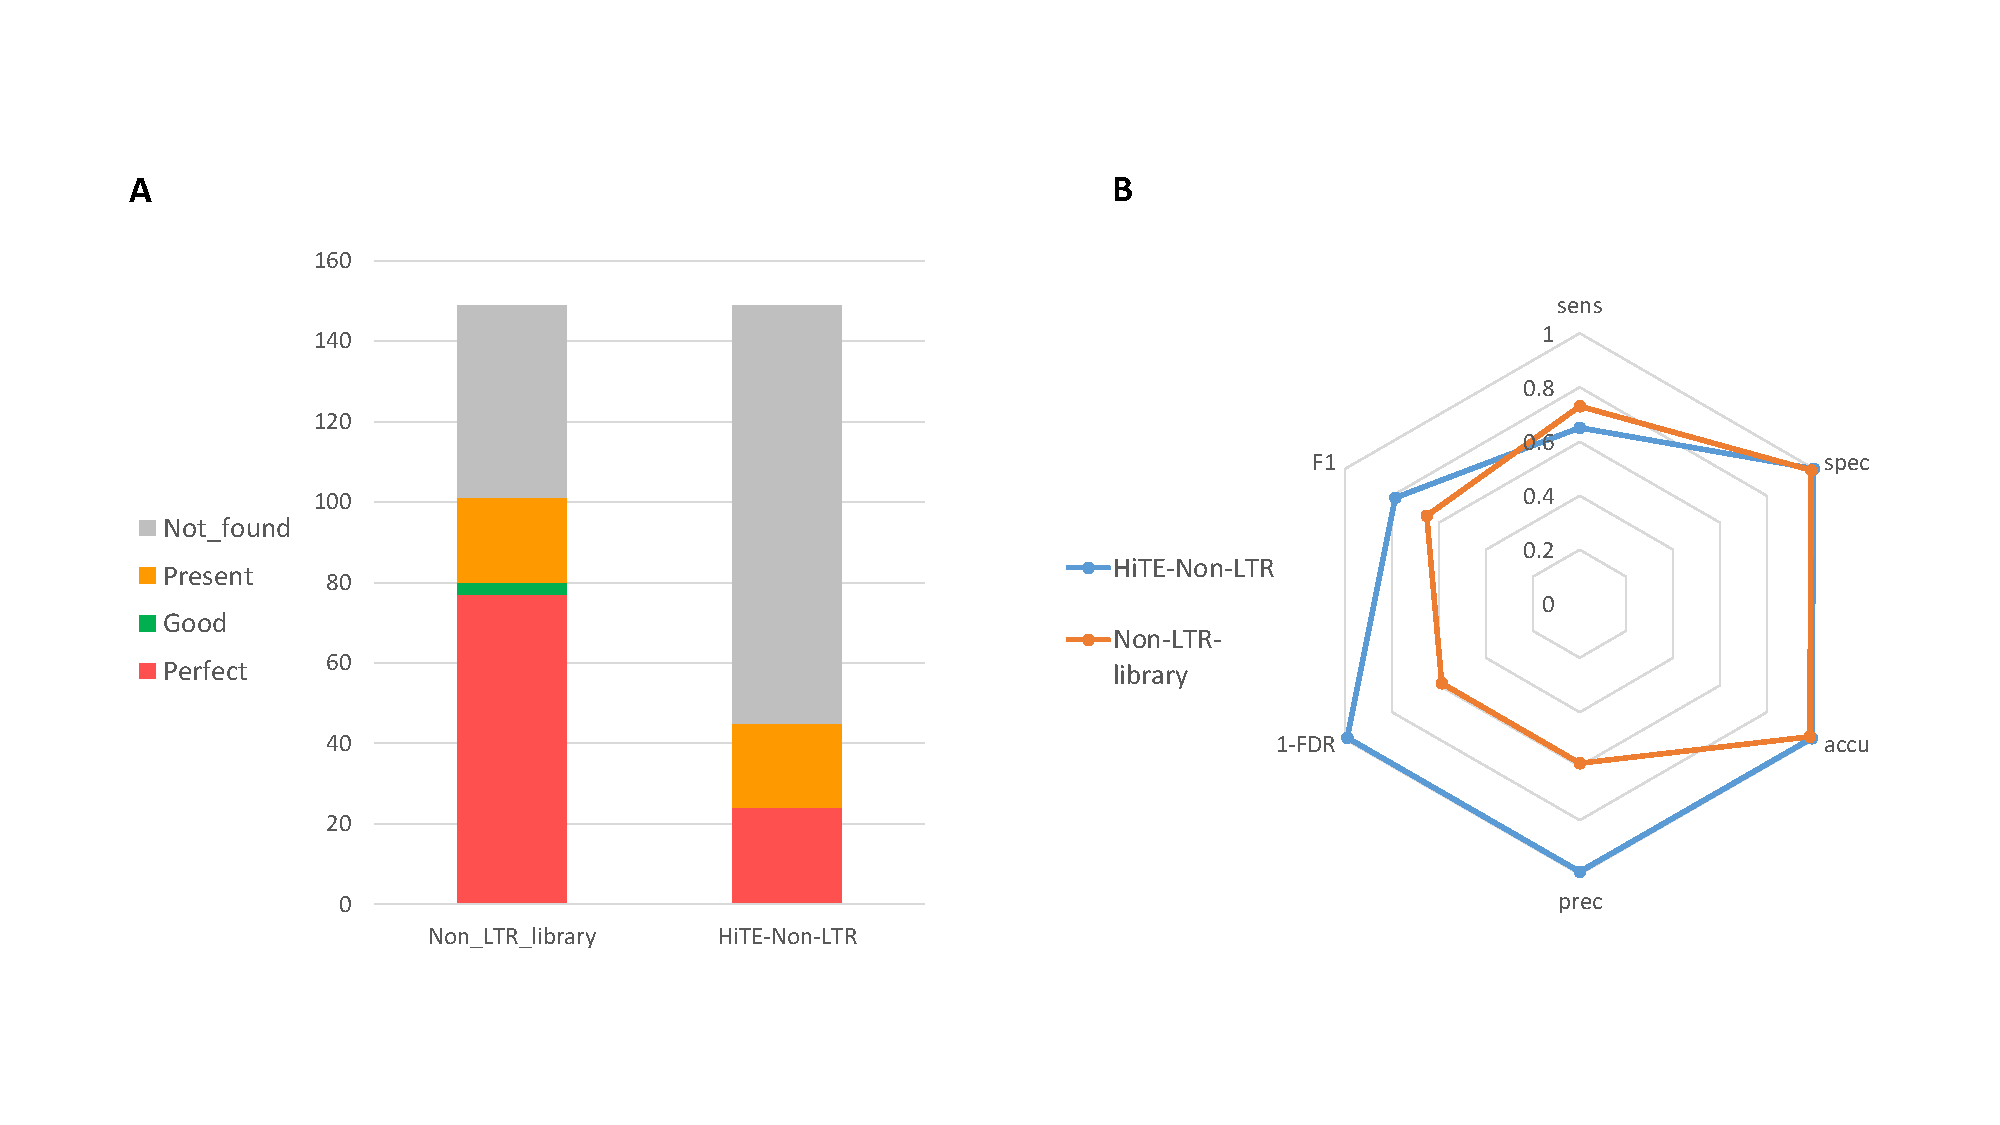
\includegraphics[width=1.0\textwidth]{figures/NonLTRResults.pdf}}
%	\caption{Performance of Non-LTR annotators. \textbf{a} the performance based on benckmarking method of RepeatModeler2 and \textbf{b} the performance based on benckmarking method of EDTA.}
%	\label{fig:non_ltr_results}
%\end{figure}
%
%\begin{figure}[h!]
%	%\centerline{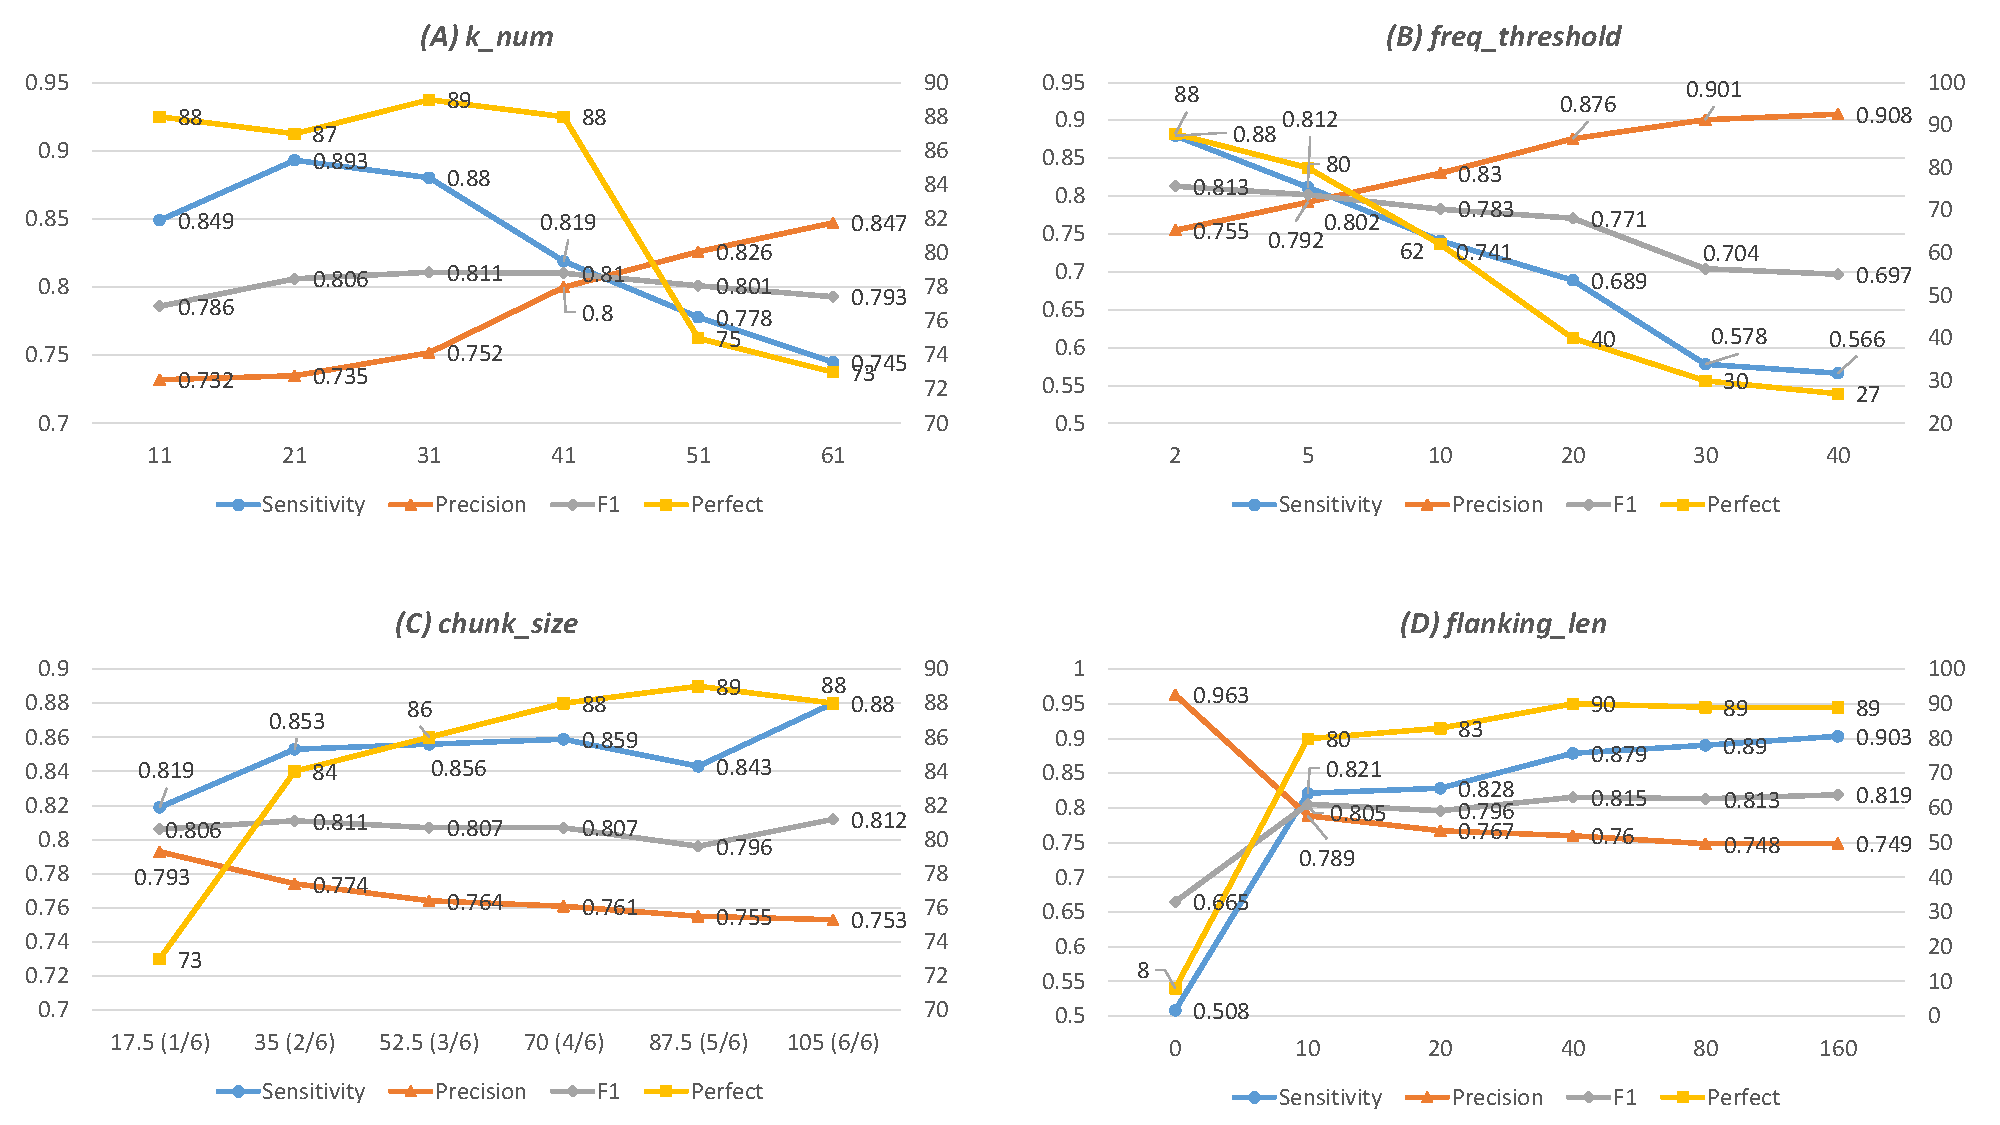
\includegraphics[width=1.0\textwidth]{figures/ParamResults.pdf}}
%	\caption{Influence of parameter changes on results. \textbf{a} influence of k\_num parameter on results; \textbf{b} influence of freq\_threshold parameter on results; \textbf{c} influence of chunk\_size parameter on results; and \textbf{d} influence of flanking\_len parameter on results.}
%	\label{fig:param_results}
%\end{figure}
%%%%%%%%%%%%%%%%%%%%%%%%%%%%%%%%%%%
%%                               %%
%% Tables                        %%
%%                               %%
%%%%%%%%%%%%%%%%%%%%%%%%%%%%%%%%%%%

%% Use of \listoftables is discouraged.
%%
\section*{Tables}
%\begin{table}[h!]
%\caption{Sample table title. This is where the description of the table should go}
%  \begin{tabular}{cccc}
%    \hline
%    & B1  &B2   & B3\\ \hline
%    A1 & 0.1 & 0.2 & 0.3\\
%    A2 & ... & ..  & .\\
%    A3 & ..  & .   & .\\ \hline
%  \end{tabular}
%\end{table}

%\begin{table}[h!]
%	\caption{TE content in the benchmarking genomes.}\label{repbase_genome}
%	\setlength{\tabcolsep}{2.5 mm}{
%		\renewcommand{\arraystretch}{1.5}
%		\begin{tabular}{cccccc}
%			\hline
%			& & Class & RepBase26.05  & Number of elements & Total (\%)\\ \hline
%			\multirow{5}{*}{O. sativa*} &
%			LTR & Class I & 88.4 Mb & 46595 & 23.61 \\
%			& Non-LTR & Class I & 5.7 Mb & 13381 & 1.51 \\
%			& TIR & Class II  & 67.7 Mb & 230281 & 18.09 \\
%			& Helitron & Class II & 17.2 Mb & 66469 & 4.60 \\
%			& Total & - & 179.0 Mb & 356726 & 47.81 \\ \hline  
%			\multirow{5}{*}{C. briggsae*} &
%			LTR & Class I & 0.2 Mb & 234 & 0.2 \\
%			& Non-LTR & Class I & 0.9 Mb & 3085 & 0.59 \\
%			& TIR & Class II  & 14.5 Mb & 68146 & 13.41 \\
%			& Helitron & Class II & 1.8 Mb & 8509 & 1.63 \\
%			& Total & - & 17.4 Mb & 79974 & 15.83 \\ \hline
%			\multirow{5}{*}{D. melanogaster*} &
%			LTR & Class I & 19.9 Mb & 21050 & 11.78 \\
%			& Non-LTR & Class I & 10.8 Mb & 15428 & 6.37 \\
%			& TIR & Class II  & 2.6 Mb & 6204 & 1.53 \\
%			& Helitron & Class II & 1.0 Mb & 4822 & 0.60 \\
%			& Total & - & 34.2 Mb & 47504 & 20.28 \\ \hline
%			\multirow{5}{*}{D. rerio*} &
%			LTR & Class I & 119.0 Mb & 296556 & 7.09 \\
%			& Non-LTR & Class I & 74.3 Mb & 215393 & 4.42 \\
%			& TIR & Class II  & 719.4 Mb & 3372500 & 42.84 \\
%			& Helitron & Class II & 50.5 Mb & 178913 & 3.01 \\
%			& Total & - & 963.2 Mb & 4063362 & 57.36 \\ \hline
%		\end{tabular}
%		\begin{tablenotes}
%			\item[1] *Oryza sativa Japonica Group ``assembly IRGSP-1.0"
%			\item[2] *Caenorhabditis briggsae ``assembly CB4"
%			\item[3] *Drosophila melanogaster ``assembly Release 6 plus ISO1 MT"
%			\item[4] *Danio rerio ``assembly GRCz11"
%		\end{tablenotes}
%	}
%\end{table}

%%%%%%%%%%%%%%%%%%%%%%%%%%%%%%%%%%%
%%                               %%
%% Additional Files              %%
%%                               %%
%%%%%%%%%%%%%%%%%%%%%%%%%%%%%%%%%%%

\section*{Additional Files}
  \subsection*{Additional file 1 --- Supplementary Materials}

  \subsection*{Additional file 2 --- Supplementary Data}
    \textbf{Table S1.} Details of performance among general-purpose repeat annotators. \textbf{Table S2.} Details of performance among all types of TE annotators based on O. sativa. \textbf{Table S3.} Time and resource consumption. \textbf{Table S4.} Details of tools and parameters used in benchmarking and HiTE.
    
\end{backmatter}
\end{document}
